\section{Introduction\label{sec:asym-intro}}

This chapter demonstrates how the surface symmetry of a zigzag grating may be used to manipulate both the coupling of light to SPPs, and the band structure of SPPs on the zigzag surface. Much of the discussion in this chapter draws parallels with the zigzag grating explored in chapter \ref{c:zigzag}. The zigzag grating explored in chapter \ref{c:zigzag} will be referred to as a `symmetric' zigzag grating, due to the presence of mirror symmetry in the $yz$ plane. The zigzag grating which shall be the topic of this chapter has no such symmetry, and so will be referred to as an `asymmetric' zigzag grating. The asymmetric zigzag grating is formed from a set of sub-wavelength (non-diffracting) grooves that are zigzagged along their length such that the zigzag apexes do not lie at high symmetry points within the rectangular unit cell. The length scale of the zigzag pitch is on the order of the wavelength of impinging light, so that the grating may diffractively couple to SPPs.

The resulting structure is 2D chiral, much like `fish-scale' nanowires reported previously, \cite{Plum2010,Genet2008,Schwanecke2008,Kao2010,Fedotov2007a} but we restrict our investigation to the excitation and band structure of SPPs along such a surface, rather than any optical chirality exhibited by the grating.

In this chapter it is demonstrated that any polarisation of light may couple to the SPP modes on a zigzag grating which possesses no mirror symmetry. Furthermore, it is shown that light of different polarisation will couple to the exact same SPP modes, and these SPP modes propagate in the same direction, regardless of polarisation. This latter point is subtle, but important, as previous work has shown that the excitation of SPPs on crossed bigratings may also couple arbitrary polarised light into SPPs on the surface \cite{Popov2008,Hibbins1998,Watts1996}, but in this case different incident polarisations states excite different, or multiple, SPPs. The coupling of arbitrarily polarised light to SPPs on deep lamella gratings has also been shown \cite{Bonod2008}, where the SPP modes evolve to become similar in character to localised cavity modes. In the zigzag case presented here, light of any arbitrary polarisation is coupled to the same SPP modes, and the energy flow across the surface is mediated by these SPPs travelling in a single direction only. This makes these asymmetric gratings an excellent possible component for efficient plasmonic circuitry \cite{Ozbay2006a}.

The manipulation of available Fourier components by altering the geometry of the asymmetric zigzag surface also allows the design of the SPP band structure on such gratings. We find in section \ref{sec:asym-bandstructure}, theoretically and experimentally, how the asymmetric zigzag pattern can cause band gaps to form between the $+\mathbf{k}_{gx}$ and $-\mathbf{k}_{gx}$ scattered SPPs, by providing a direct scattering mechanism by which they may interact. We also show in section \ref{sec:asym-bandstructure} how the degeneracy of standing wave solutions at the first BZ boundary, described in chapter \ref{c:zigzag} for the symmetric case, is destroyed in the asymmetric zigzag case. The coupling of light to the two energetically dissimilar standing wave states is also investigated, as the high energy solution is found to be poorly coupled to light compared to the lower energy mode.

Finally, highly anisotropic propagation of SPPs along zigzag gratings, when combined with the possible large band gap at the first BZ boundary, causes the formation of a full-plasmonic band gap, for which propagation of SPP for a given frequency range is forbidden in all directions. Full plasmonic band-gaps have shown potential in surface plasmon based lasers \cite{Okamoto2004,H'Dhili2011,Okamoto2008,Berini2011}, and are usually only found in systems with hexagonal \cite{Kitson1996}, not rectangular, symmetry.

\section{The Asymmetric Zigzag Grating\label{sec:asym-about}}

\begin{figure}[h]
\begin{center}
\input{figure-asymmetric-zigzag-coordinated-latexannotations.pdf_tex}
\end{center}
\caption[Coordinate system for the asymmetric zigzag grating.]{Coordinate system for the asymmetric zigzag grating. The experimental parameters were $\lambda_{gx}=600\:\nano\metre, \lambda_{gy}=150\:\nano\metre, d\approx 40\:\nano\metre,$ and $\delta=150\:\nano\metre$ . \label{fig:asymzz-coords}}
\end{figure}

The coordinate system used for the asymmetric zigzag grating is shown in figure \ref{fig:asymzz-coords}. Light impinges on the surface at a polar angle $\theta$ in the plane of incidence that lies at an angle $\phi$, with $\phi=0^\circ$ containing the primary grating vector, $k_{gx}=2\pi\hat{\mathbf{x}}/\lambda_{gx}$. The polarisation of the light is defined as TM polarised light when the electric vector is in the plane of incidence, and TE polarised light when the electric vector lies perpendicular to the plane of incidence. The offset of the zigzag apex, $\delta$ is the distance between the centre of the unit cell and the closest apex, as shown. It is this offset that removes the mirror symmetry of the zigzag grating. The grating grooves are of a depth $d$. The target parameters (for fabrication) used in this chapter are as follows:  ${\lambda_{gx}=600\:\nano\metre}, {\lambda_{gy}=150\:\nano\metre}, {d\approx 40\:\nano\metre}$ and ${\delta=150 \:\nano\metre}$ with the grating made of silver. The zigzag amplitude is defined as the distance between a low and high apex of the zigzag divided by two.  

\begin{figure}
\begin{center}
\subfigure[Symmetric]{
\includegraphics[width=0.45\linewidth]{./hfss-bandgaps/figure-symmetric-unitcell}}
\subfigure[Asymmetric]{
\includegraphics[width=0.45\linewidth]{figure-asymmetric-unitcell-extralabels}}
\end{center}
\caption[Two possible unit cells for a zigzag grating: symmetric and asymmetric.]{Two possible unit cells for a zigzag grating. (a) The grating unit cell explored previously in chapter \ref{c:zigzag}. (b) An asymmetrical zigzag grating, with the central apex of the zigzag shifted by $150\:\nano\metre$. This shift removes the mirror-symmetry of the zigzag.\label{fig:azz-unitcells}}
\end{figure}

The zigzag grating presented in this chapter has a reduced symmetry from the zigzag grating presented in chapter \ref{c:zigzag}. This is achieved by offsetting one of the zigzag apexes along $\hat{\mathbf{x}}$ with respect to the centre of the unit cell by a distance $\delta= 150 \:\nano\metre$, as shown in figure \ref{fig:azz-unitcells}. This produces a grating structure with no mirror or rotational symmetry in real space, but still having a rectangular unit cell and a rectangular lattice in reciprocal space. For ease of description, we refer to the `left hand side' of the grating, the region ${0\:\nano\metre<x<450\:\nano\metre}$ (to the left of the apex), as `region 1' and the right hand side of between $450\:\nano\metre<x<600\:\nano\metre$ as `region 2'.

\begin{figure}
\begin{center}
\subfigure[Master]{\includegraphics[width=0.49\linewidth]{sem-master}}
\subfigure[Metal grating replica]{\includegraphics[width=0.49\linewidth]{pic_016}}
\end{center}
\caption[Scanning electron micrographs of an asymmetric zigzag silicon master and the template stripped sample in silver.]{Scanning electron micrographs of (a) The asymmetric zigzag silicon master and (b) the template stripped sample in silver.\label{fig:azz-sems}}
\end{figure}
The samples are produced using electron beam lithography as detailed in chapter \ref{c:experimentalmethods}. Scanning electron micrographs of the silicon master and the template stripped sample in silver are shown in figure \ref{fig:azz-sems}, with the following parameters: $\lambda_{gx}=597\pm 5\:\nano\metre, \lambda_{gy}=156\pm 9\:\nano\metre, d\approx 40\:\nano\metre, \delta=126\pm 5\:\nano\metre$ with a zigzag amplitude of $121\pm 3\:\nano\metre$. 

Due to the template stripping method of fabrication, the produced silver grating is an inverse duplicate of the grating master. The master SEM \ref{fig:azz-sems} also shows a clear stitching error on the right of the SEM, where the zigzag continuity has been broken. These stitching errors are infrequent and, over the area of the grating, do not effect the optical response greatly.

Notice that the zigzag amplitude of the sample is greater than that of the unit cell in figure \ref{fig:azz-unitcells}. The experimental and modelled results will show that since an increased zigzag amplitude alone does not alter the symmetry of the zigzag surface, the fundamental optical response of the grating is unaltered. For simplicity in understanding only consideration of the unit cell in figure \ref{fig:azz-unitcells} is necessary to gain an insight into the optical response of our sample.

\section{The Coupling of Polarised Light to SPPs on an Asymmetric Zigzag Grating\label{sec:asym-lightcoupling}}
\subsection{Theory}

In chapter \ref{c:zigzag}, it was shown that a zigzag grating possesses a surface profile that allows surface charge density oscillations to be induced by either TE or TM polarised light. This is because both TE and TM light provide a component of the incident electric field that lies normal to some part of the metal surface. For the case of the grating examined in chapter \ref{c:zigzag}, the field profiles of these induced charge density oscillations were constrained by the symmetry of the surface so that the wavevector of SPPs  coupling to TE polarised light are only the odd-orders of diffraction, while the TM polarised light could only match the wavevector of even-order diffracted SPPs. These coupling conditions can be deduced from the plane wave expansion equations \ref{eq:etm} and \ref{eq:ete}. Since the functions $E_{TE}$ and $E_{TM}$ will possess the same mirror symmetry as the surface function,  so the Fourier expansions of  $E_{TE}$ and $E_{TM}$ only require every-other Fourier coefficient to fully describe the functions. This is what leads to the polarisation selectivity of this type of grating.

However, by removing the mirror symmetry of the zigzag surface the equivalent expressions for $E_{TE}$ and $E_{TM}$ in the asymmetric zigzag case will themselves not be mirror symmetric. We can demonstrate this simply by considering the E field for normal incident light, as shown diagrammatically in figure \ref{fig:asymcouplingcartoon}. 

\begin{figure}
\def\svgwidth{1\linewidth}
\input{figure-asymzz-coupling.pdf_tex}
\caption[A schematic of the electric field lines in the grooves of an asymmetric zigzag grating for two polarisation cases.]{(above) A schematic of the electric field lines in the grooves (black arrows) of an asymmetric zigzag grating for two polarisation cases, and the resulting $E_x$ component (red arrows). The points connecting the apexes lead to fixed points of zero $E_x$, leading to an asymmetric field distribution along the plane of propagation (bottom).\label{fig:asymcouplingcartoon}}
\end{figure}

In this figure, the possible electric fields across the zigzag grooves are shown for two electric vectors, one in the $x$ direction (left), and one in the $y$ direction (right). The electric vectors pointing along a single axes like this represents two orthogonal polarisations at a single instant in time when the light in incident normal to the surface. The plane of incidence at $\theta=0^\circ$ is not defined, as the wavevector possesses no component in the surface plane $xy$, but for $\phi=0^\circ$ and for a very small polar angle $\theta$, the polarisation is defined as TE for the vector lying along the $x$ axis (right) and TM for the vector lying along the $y$ axis (left), so we shall refer to the left-hand diagram as the TE polarised case, and the right-hand side as the TM polarised case.

The figure shows that for the electric vector oriented along the $x$ or the $y$ axis, the incident field may provide a normal component to the grating surface and so induce surface charge. Because of the surface geometry, charge density oscillations may be induced on the grating surface and so there exists a possibility of exciting SPPs. Since in our experiments $\lambda_{gy}$ is sub-wavelength, we need only consider the electric field profile along the $x$ axis, as this is the axis along which momentum conservation requires diffracted SPPs to propagate. The $x$-components of the electric fields in the grooves are shown as red arrows in the figure. Possible example functions for each polarisation which fulfil the asymmetry criteria of the grating are shown in the lower half of figure \ref{fig:asymcouplingcartoon}, which have been deduced from the  diagrams above. These functions are neither odd nor even, both possessing only the symmetry of the grating (a rotation and translation operation or `glide operation'), and will in general vary in amplitude in the two regions. 

The key point illustrated in this figure is that the normal component of electric field varies in the $x$-direction asymmetrically with respect to the unit cell. This is because the $x$-component of the electric field originating from charge carriers must be pinned to zero at the zigzag apexes by the geometry of the grating, and the position of these apexes do not lie at points of any high-symmetry. The plane wave expansion description of such general diffracted SPPs fields on such a surface will necessarily contain all Fourier components including both odd and even harmonics, for both polarisation cases. 

In chapter \ref{c:zigzag}, we calculated the Fourier series of $E_{TE} (\equiv E_x^{TE})$ and $E_{TM} (\equiv E_x^{TM})$ by first deriving the electric field from the expected induced surface charge along $x$ as the functions $E_x^{TE}$ and $E_x^{TM}$. Examination of the plane wave expansion of these fields determines the coupling of light to different orders of diffracted SPP. In the asymmetric case, the strict derivation of $E_x^{TE}$ and $E_x^{TM}$ is difficult, due to the lack of symmetry in the grating's geometry. 
We can instead construct an example function from careful consideration of the conditions an $E_x$ field must possess along such a grating. We place five constraints on any function we choose: (1) That the function must be continuous along $x$, with no sharp discontinuities or undefined points; (2) that the function is periodic, with a period equal to that of a single grating period, $\lambda_{gx}$; (3) that the function must equal $E_x=0$ at the $x$ coordinates which correspond to a zigzag apex; (4) that between these zeros, the magnitude of $E_x$ will reach a maximum value determined by the polarisation and local geometry and; (5) the resulting function must possess the same symmetry as the grating (a single $C_2$ rotation operation).

Such a function must be defined piecewise, with the same symmetry as the intuitive example functions drawn in figure \ref{fig:as-piecewisefuncs}. Choosing a simple sine wave for each region, the function we shall use is defined as,
\begin{align}
E_x^{TM}(x) &= \begin{cases} E_{x_1}^{TM*}(1+\sin{(-\frac{L}{2}+\frac{2\pi x}{(L+\delta)})}) &0<x<L+\delta \\
 E_{x_2}^{TM*}(-1+\sin{(\frac{L}{2}+\frac{2\pi (x-L-\delta)}{(L-\delta)})}) & L+\delta<x<2L \end{cases} 
\\
E_x^{TE}(x) &= \begin{cases} E_{x_1}^{TE*}(1+\sin{(-\frac{L}{2}+\frac{2\pi x}{(L+\delta)})}) &0<x<L+\delta \\
 -E_{x_2}^{TE*}(-1+\sin{(\frac{L}{2}+\frac{2\pi (x-L-\delta)}{(L-\delta)})})& L+\delta<x<2L \end{cases} 
\end{align} 
Where $2L=\lambda_{gx}$. The variable $\delta$ represents a positive offset of the central zero point from $x=L$ and the function is defined as periodic with a period $2L$. These functions are plotted in figure \ref{fig:as-piecewisefuncs}

\begin{figure}
\begin{center}
% Created by tikzDevice version 0.6.2-92-0ad2792 on 2013-02-01 15:20:33
% !TEX encoding = UTF-8 Unicode
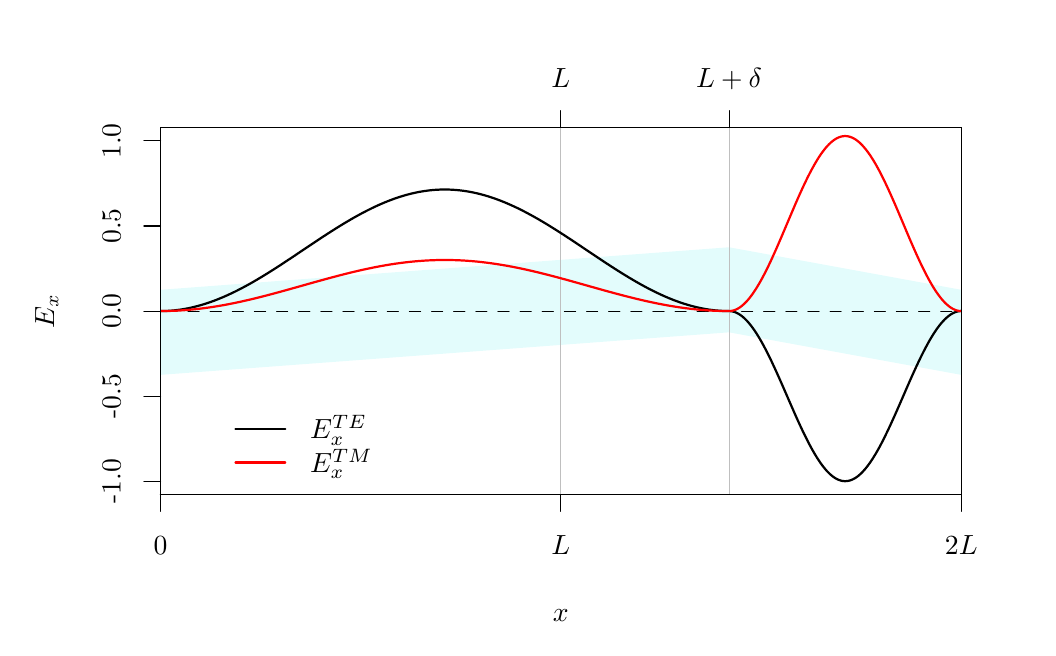
\begin{tikzpicture}[x=1pt,y=1pt]
\definecolor[named]{fillColor}{rgb}{1.00,1.00,1.00}
\path[use as bounding box,fill=fillColor,fill opacity=0.00] (0,0) rectangle (361.35,216.81);
\begin{scope}
\path[clip] (  0.00,  0.00) rectangle (361.35,216.81);
\definecolor[named]{drawColor}{rgb}{0.00,0.00,0.00}

\path[draw=drawColor,line width= 0.4pt,line join=round,line cap=round] ( 48.00, 52.92) -- ( 48.00,175.89);

\path[draw=drawColor,line width= 0.4pt,line join=round,line cap=round] ( 48.00, 52.92) -- ( 42.00, 52.92);

\path[draw=drawColor,line width= 0.4pt,line join=round,line cap=round] ( 48.00, 83.66) -- ( 42.00, 83.66);

\path[draw=drawColor,line width= 0.4pt,line join=round,line cap=round] ( 48.00,114.40) -- ( 42.00,114.40);

\path[draw=drawColor,line width= 0.4pt,line join=round,line cap=round] ( 48.00,145.15) -- ( 42.00,145.15);

\path[draw=drawColor,line width= 0.4pt,line join=round,line cap=round] ( 48.00,175.89) -- ( 42.00,175.89);

\node[text=drawColor,rotate= 90.00,anchor=base,inner sep=0pt, outer sep=0pt, scale=  1.00] at ( 33.60, 52.92) {-1.0};

\node[text=drawColor,rotate= 90.00,anchor=base,inner sep=0pt, outer sep=0pt, scale=  1.00] at ( 33.60, 83.66) {-0.5};

\node[text=drawColor,rotate= 90.00,anchor=base,inner sep=0pt, outer sep=0pt, scale=  1.00] at ( 33.60,114.40) {0.0};

\node[text=drawColor,rotate= 90.00,anchor=base,inner sep=0pt, outer sep=0pt, scale=  1.00] at ( 33.60,145.15) {0.5};

\node[text=drawColor,rotate= 90.00,anchor=base,inner sep=0pt, outer sep=0pt, scale=  1.00] at ( 33.60,175.89) {1.0};

\path[draw=drawColor,line width= 0.4pt,line join=round,line cap=round] ( 48.00, 48.00) --
	(337.35, 48.00) --
	(337.35,180.81) --
	( 48.00,180.81) --
	( 48.00, 48.00);
\end{scope}
\begin{scope}
\path[clip] (  0.00,  0.00) rectangle (361.35,216.81);
\definecolor[named]{drawColor}{rgb}{0.00,0.00,0.00}

\node[text=drawColor,anchor=base,inner sep=0pt, outer sep=0pt, scale=  1.00] at (192.68,  2.40) {$x$};

\node[text=drawColor,rotate= 90.00,anchor=base,inner sep=0pt, outer sep=0pt, scale=  1.00] at (  9.60,114.40) {$E_x$};
\end{scope}
\begin{scope}
\path[clip] (  0.00,  0.00) rectangle (361.35,216.81);
\definecolor[named]{drawColor}{rgb}{0.00,0.00,0.00}

\path[draw=drawColor,line width= 0.4pt,line join=round,line cap=round] ( 48.00, 48.00) -- (337.35, 48.00);

\path[draw=drawColor,line width= 0.4pt,line join=round,line cap=round] ( 48.00, 48.00) -- ( 48.00, 42.00);

\path[draw=drawColor,line width= 0.4pt,line join=round,line cap=round] (192.67, 48.00) -- (192.67, 42.00);

\path[draw=drawColor,line width= 0.4pt,line join=round,line cap=round] (337.35, 48.00) -- (337.35, 42.00);

\node[text=drawColor,anchor=base,inner sep=0pt, outer sep=0pt, scale=  1.00] at ( 48.00, 26.40) {0};

\node[text=drawColor,anchor=base,inner sep=0pt, outer sep=0pt, scale=  1.00] at (192.67, 26.40) {$L$};

\node[text=drawColor,anchor=base,inner sep=0pt, outer sep=0pt, scale=  1.00] at (337.35, 26.40) {$2L$};
\end{scope}
\begin{scope}
\path[clip] ( 48.00, 48.00) rectangle (337.35,180.81);
\definecolor[named]{fillColor}{rgb}{0.89,0.99,0.99}

\path[fill=fillColor] ( 48.00, 91.35) --
	( 48.00,122.09) --
	(253.44,137.46) --
	(337.35,122.09) --
	(337.35, 91.35) --
	(253.44,106.72) --
	cycle;
\definecolor[named]{drawColor}{rgb}{0.75,0.75,0.75}

\path[draw=drawColor,line width= 0.4pt,line join=round,line cap=round] (192.67,  0.00) --
	(192.67,216.81);

\path[draw=drawColor,line width= 0.4pt,line join=round,line cap=round] (253.44,  0.00) --
	(253.44,216.81);
\end{scope}
\begin{scope}
\path[clip] (  0.00,  0.00) rectangle (361.35,216.81);
\definecolor[named]{drawColor}{rgb}{0.00,0.00,0.00}

\path[draw=drawColor,line width= 0.4pt,line join=round,line cap=round] (192.67,180.81) -- (253.44,180.81);

\path[draw=drawColor,line width= 0.4pt,line join=round,line cap=round] (192.67,180.81) -- (192.67,186.81);

\path[draw=drawColor,line width= 0.4pt,line join=round,line cap=round] (253.44,180.81) -- (253.44,186.81);

\node[text=drawColor,anchor=base,inner sep=0pt, outer sep=0pt, scale=  1.00] at (192.67,195.21) {$L$};

\node[text=drawColor,anchor=base,inner sep=0pt, outer sep=0pt, scale=  1.00] at (253.44,195.21) {$L+\delta$};
\end{scope}
\begin{scope}
\path[clip] ( 48.00, 48.00) rectangle (337.35,180.81);
\definecolor[named]{drawColor}{rgb}{0.00,0.00,0.00}

\path[draw=drawColor,line width= 0.4pt,dash pattern=on 4pt off 4pt ,line join=round,line cap=round] (  1.95,114.40) --
	(361.35,114.40);

\path[draw=drawColor,line width= 0.8pt,line join=round,line cap=round] ( 48.00,114.40) --
	( 48.29,114.41) --
	( 48.58,114.41) --
	( 48.87,114.41) --
	( 49.16,114.42) --
	( 49.45,114.43) --
	( 49.74,114.44) --
	( 50.03,114.45) --
	( 50.32,114.46) --
	( 50.61,114.47) --
	( 50.90,114.49) --
	( 51.19,114.51) --
	( 51.48,114.53) --
	( 51.77,114.55) --
	( 52.05,114.57) --
	( 52.34,114.60) --
	( 52.63,114.63) --
	( 52.92,114.65) --
	( 53.21,114.68) --
	( 53.50,114.72) --
	( 53.79,114.75) --
	( 54.08,114.78) --
	( 54.37,114.82) --
	( 54.66,114.86) --
	( 54.95,114.90) --
	( 55.24,114.94) --
	( 55.53,114.98) --
	( 55.82,115.03) --
	( 56.11,115.08) --
	( 56.40,115.13) --
	( 56.69,115.18) --
	( 56.98,115.23) --
	( 57.27,115.28) --
	( 57.56,115.34) --
	( 57.85,115.39) --
	( 58.14,115.45) --
	( 58.43,115.51) --
	( 58.72,115.57) --
	( 59.01,115.64) --
	( 59.30,115.70) --
	( 59.59,115.77) --
	( 59.88,115.84) --
	( 60.16,115.91) --
	( 60.45,115.98) --
	( 60.74,116.05) --
	( 61.03,116.13) --
	( 61.32,116.20) --
	( 61.61,116.28) --
	( 61.90,116.36) --
	( 62.19,116.44) --
	( 62.48,116.52) --
	( 62.77,116.61) --
	( 63.06,116.69) --
	( 63.35,116.78) --
	( 63.64,116.87) --
	( 63.93,116.96) --
	( 64.22,117.05) --
	( 64.51,117.15) --
	( 64.80,117.24) --
	( 65.09,117.34) --
	( 65.38,117.43) --
	( 65.67,117.53) --
	( 65.96,117.63) --
	( 66.25,117.74) --
	( 66.54,117.84) --
	( 66.83,117.95) --
	( 67.12,118.05) --
	( 67.41,118.16) --
	( 67.70,118.27) --
	( 67.99,118.38) --
	( 68.27,118.49) --
	( 68.56,118.61) --
	( 68.85,118.72) --
	( 69.14,118.84) --
	( 69.43,118.96) --
	( 69.72,119.08) --
	( 70.01,119.20) --
	( 70.30,119.32) --
	( 70.59,119.44) --
	( 70.88,119.57) --
	( 71.17,119.69) --
	( 71.46,119.82) --
	( 71.75,119.95) --
	( 72.04,120.08) --
	( 72.33,120.21) --
	( 72.62,120.34) --
	( 72.91,120.48) --
	( 73.20,120.61) --
	( 73.49,120.75) --
	( 73.78,120.88) --
	( 74.07,121.02) --
	( 74.36,121.16) --
	( 74.65,121.30) --
	( 74.94,121.44) --
	( 75.23,121.59) --
	( 75.52,121.73) --
	( 75.81,121.88) --
	( 76.10,122.03) --
	( 76.38,122.17) --
	( 76.67,122.32) --
	( 76.96,122.47) --
	( 77.25,122.62) --
	( 77.54,122.78) --
	( 77.83,122.93) --
	( 78.12,123.08) --
	( 78.41,123.24) --
	( 78.70,123.40) --
	( 78.99,123.55) --
	( 79.28,123.71) --
	( 79.57,123.87) --
	( 79.86,124.03) --
	( 80.15,124.19) --
	( 80.44,124.35) --
	( 80.73,124.52) --
	( 81.02,124.68) --
	( 81.31,124.85) --
	( 81.60,125.01) --
	( 81.89,125.18) --
	( 82.18,125.35) --
	( 82.47,125.52) --
	( 82.76,125.69) --
	( 83.05,125.86) --
	( 83.34,126.03) --
	( 83.63,126.20) --
	( 83.92,126.37) --
	( 84.20,126.55) --
	( 84.49,126.72) --
	( 84.78,126.90) --
	( 85.07,127.07) --
	( 85.36,127.25) --
	( 85.65,127.43) --
	( 85.94,127.60) --
	( 86.23,127.78) --
	( 86.52,127.96) --
	( 86.81,128.14) --
	( 87.10,128.32) --
	( 87.39,128.50) --
	( 87.68,128.69) --
	( 87.97,128.87) --
	( 88.26,129.05) --
	( 88.55,129.24) --
	( 88.84,129.42) --
	( 89.13,129.60) --
	( 89.42,129.79) --
	( 89.71,129.98) --
	( 90.00,130.16) --
	( 90.29,130.35) --
	( 90.58,130.54) --
	( 90.87,130.72) --
	( 91.16,130.91) --
	( 91.45,131.10) --
	( 91.74,131.29) --
	( 92.03,131.48) --
	( 92.31,131.67) --
	( 92.60,131.86) --
	( 92.89,132.05) --
	( 93.18,132.24) --
	( 93.47,132.43) --
	( 93.76,132.62) --
	( 94.05,132.82) --
	( 94.34,133.01) --
	( 94.63,133.20) --
	( 94.92,133.39) --
	( 95.21,133.59) --
	( 95.50,133.78) --
	( 95.79,133.97) --
	( 96.08,134.17) --
	( 96.37,134.36) --
	( 96.66,134.55) --
	( 96.95,134.75) --
	( 97.24,134.94) --
	( 97.53,135.14) --
	( 97.82,135.33) --
	( 98.11,135.52) --
	( 98.40,135.72) --
	( 98.69,135.91) --
	( 98.98,136.11) --
	( 99.27,136.30) --
	( 99.56,136.50) --
	( 99.85,136.69) --
	(100.14,136.89) --
	(100.42,137.08) --
	(100.71,137.27) --
	(101.00,137.47) --
	(101.29,137.66) --
	(101.58,137.86) --
	(101.87,138.05) --
	(102.16,138.24) --
	(102.45,138.44) --
	(102.74,138.63) --
	(103.03,138.83) --
	(103.32,139.02) --
	(103.61,139.21) --
	(103.90,139.40) --
	(104.19,139.60) --
	(104.48,139.79) --
	(104.77,139.98) --
	(105.06,140.17) --
	(105.35,140.36) --
	(105.64,140.56) --
	(105.93,140.75) --
	(106.22,140.94) --
	(106.51,141.13) --
	(106.80,141.32) --
	(107.09,141.51) --
	(107.38,141.69) --
	(107.67,141.88) --
	(107.96,142.07) --
	(108.25,142.26) --
	(108.53,142.45) --
	(108.82,142.63) --
	(109.11,142.82) --
	(109.40,143.00) --
	(109.69,143.19) --
	(109.98,143.37) --
	(110.27,143.56) --
	(110.56,143.74) --
	(110.85,143.92) --
	(111.14,144.11) --
	(111.43,144.29) --
	(111.72,144.47) --
	(112.01,144.65) --
	(112.30,144.83) --
	(112.59,145.01) --
	(112.88,145.19) --
	(113.17,145.37) --
	(113.46,145.54) --
	(113.75,145.72) --
	(114.04,145.89) --
	(114.33,146.07) --
	(114.62,146.24) --
	(114.91,146.42) --
	(115.20,146.59) --
	(115.49,146.76) --
	(115.78,146.93) --
	(116.07,147.10) --
	(116.35,147.27) --
	(116.64,147.44) --
	(116.93,147.61) --
	(117.22,147.77) --
	(117.51,147.94) --
	(117.80,148.11) --
	(118.09,148.27) --
	(118.38,148.43) --
	(118.67,148.59) --
	(118.96,148.76) --
	(119.25,148.92) --
	(119.54,149.07) --
	(119.83,149.23) --
	(120.12,149.39) --
	(120.41,149.55) --
	(120.70,149.70) --
	(120.99,149.85) --
	(121.28,150.01) --
	(121.57,150.16) --
	(121.86,150.31) --
	(122.15,150.46) --
	(122.44,150.61) --
	(122.73,150.76) --
	(123.02,150.90) --
	(123.31,151.05) --
	(123.60,151.19) --
	(123.89,151.33) --
	(124.18,151.48) --
	(124.46,151.62) --
	(124.75,151.76) --
	(125.04,151.89) --
	(125.33,152.03) --
	(125.62,152.17) --
	(125.91,152.30) --
	(126.20,152.43) --
	(126.49,152.57) --
	(126.78,152.70) --
	(127.07,152.83) --
	(127.36,152.95) --
	(127.65,153.08) --
	(127.94,153.21) --
	(128.23,153.33) --
	(128.52,153.45) --
	(128.81,153.58) --
	(129.10,153.70) --
	(129.39,153.81) --
	(129.68,153.93) --
	(129.97,154.05) --
	(130.26,154.16) --
	(130.55,154.28) --
	(130.84,154.39) --
	(131.13,154.50) --
	(131.42,154.61) --
	(131.71,154.71) --
	(132.00,154.82) --
	(132.29,154.93) --
	(132.57,155.03) --
	(132.86,155.13) --
	(133.15,155.23) --
	(133.44,155.33) --
	(133.73,155.43) --
	(134.02,155.52) --
	(134.31,155.62) --
	(134.60,155.71) --
	(134.89,155.80) --
	(135.18,155.89) --
	(135.47,155.98) --
	(135.76,156.07) --
	(136.05,156.15) --
	(136.34,156.23) --
	(136.63,156.32) --
	(136.92,156.40) --
	(137.21,156.48) --
	(137.50,156.55) --
	(137.79,156.63) --
	(138.08,156.70) --
	(138.37,156.78) --
	(138.66,156.85) --
	(138.95,156.92) --
	(139.24,156.98) --
	(139.53,157.05) --
	(139.82,157.11) --
	(140.11,157.18) --
	(140.40,157.24) --
	(140.68,157.30) --
	(140.97,157.36) --
	(141.26,157.41) --
	(141.55,157.47) --
	(141.84,157.52) --
	(142.13,157.57) --
	(142.42,157.62) --
	(142.71,157.67) --
	(143.00,157.72) --
	(143.29,157.76) --
	(143.58,157.80) --
	(143.87,157.84) --
	(144.16,157.88) --
	(144.45,157.92) --
	(144.74,157.96) --
	(145.03,157.99) --
	(145.32,158.03) --
	(145.61,158.06) --
	(145.90,158.09) --
	(146.19,158.11) --
	(146.48,158.14) --
	(146.77,158.16) --
	(147.06,158.19) --
	(147.35,158.21) --
	(147.64,158.23) --
	(147.93,158.24) --
	(148.22,158.26) --
	(148.50,158.27) --
	(148.79,158.29) --
	(149.08,158.30) --
	(149.37,158.31) --
	(149.66,158.31) --
	(149.95,158.32) --
	(150.24,158.32) --
	(150.53,158.32) --
	(150.82,158.32) --
	(151.11,158.32) --
	(151.40,158.32) --
	(151.69,158.31) --
	(151.98,158.31) --
	(152.27,158.30) --
	(152.56,158.29) --
	(152.85,158.28) --
	(153.14,158.26) --
	(153.43,158.25) --
	(153.72,158.23) --
	(154.01,158.21) --
	(154.30,158.19) --
	(154.59,158.17) --
	(154.88,158.15) --
	(155.17,158.12) --
	(155.46,158.09) --
	(155.75,158.07) --
	(156.04,158.03) --
	(156.33,158.00) --
	(156.61,157.97) --
	(156.90,157.93) --
	(157.19,157.89) --
	(157.48,157.86) --
	(157.77,157.82) --
	(158.06,157.77) --
	(158.35,157.73) --
	(158.64,157.68) --
	(158.93,157.64) --
	(159.22,157.59) --
	(159.51,157.54) --
	(159.80,157.48) --
	(160.09,157.43) --
	(160.38,157.37) --
	(160.67,157.32) --
	(160.96,157.26) --
	(161.25,157.20) --
	(161.54,157.13) --
	(161.83,157.07) --
	(162.12,157.00) --
	(162.41,156.94) --
	(162.70,156.87) --
	(162.99,156.80) --
	(163.28,156.72) --
	(163.57,156.65) --
	(163.86,156.58) --
	(164.15,156.50) --
	(164.44,156.42) --
	(164.72,156.34) --
	(165.01,156.26) --
	(165.30,156.18) --
	(165.59,156.09) --
	(165.88,156.00) --
	(166.17,155.92) --
	(166.46,155.83) --
	(166.75,155.74) --
	(167.04,155.64) --
	(167.33,155.55) --
	(167.62,155.45) --
	(167.91,155.36) --
	(168.20,155.26) --
	(168.49,155.16) --
	(168.78,155.06) --
	(169.07,154.96) --
	(169.36,154.85) --
	(169.65,154.75) --
	(169.94,154.64) --
	(170.23,154.53) --
	(170.52,154.42) --
	(170.81,154.31) --
	(171.10,154.20) --
	(171.39,154.08) --
	(171.68,153.97) --
	(171.97,153.85) --
	(172.26,153.73) --
	(172.55,153.61) --
	(172.83,153.49) --
	(173.12,153.37) --
	(173.41,153.24) --
	(173.70,153.12) --
	(173.99,152.99) --
	(174.28,152.86) --
	(174.57,152.74) --
	(174.86,152.60) --
	(175.15,152.47) --
	(175.44,152.34) --
	(175.73,152.21) --
	(176.02,152.07) --
	(176.31,151.93) --
	(176.60,151.80) --
	(176.89,151.66) --
	(177.18,151.52) --
	(177.47,151.38) --
	(177.76,151.23) --
	(178.05,151.09) --
	(178.34,150.94) --
	(178.63,150.80) --
	(178.92,150.65) --
	(179.21,150.50) --
	(179.50,150.35) --
	(179.79,150.20) --
	(180.08,150.05) --
	(180.37,149.90) --
	(180.65,149.75) --
	(180.94,149.59) --
	(181.23,149.43) --
	(181.52,149.28) --
	(181.81,149.12) --
	(182.10,148.96) --
	(182.39,148.80) --
	(182.68,148.64) --
	(182.97,148.48) --
	(183.26,148.32) --
	(183.55,148.15) --
	(183.84,147.99) --
	(184.13,147.82) --
	(184.42,147.66) --
	(184.71,147.49) --
	(185.00,147.32) --
	(185.29,147.15) --
	(185.58,146.98) --
	(185.87,146.81) --
	(186.16,146.64) --
	(186.45,146.47) --
	(186.74,146.29) --
	(187.03,146.12) --
	(187.32,145.95) --
	(187.61,145.77) --
	(187.90,145.59) --
	(188.19,145.42) --
	(188.48,145.24) --
	(188.76,145.06) --
	(189.05,144.88) --
	(189.34,144.70) --
	(189.63,144.52) --
	(189.92,144.34) --
	(190.21,144.16) --
	(190.50,143.98) --
	(190.79,143.80) --
	(191.08,143.61) --
	(191.37,143.43) --
	(191.66,143.24) --
	(191.95,143.06) --
	(192.24,142.87) --
	(192.53,142.69) --
	(192.82,142.50) --
	(193.11,142.31) --
	(193.40,142.13) --
	(193.69,141.94) --
	(193.98,141.75) --
	(194.27,141.56) --
	(194.56,141.37) --
	(194.85,141.18) --
	(195.14,140.99) --
	(195.43,140.80) --
	(195.72,140.61) --
	(196.01,140.42) --
	(196.30,140.23) --
	(196.59,140.04) --
	(196.87,139.85) --
	(197.16,139.65) --
	(197.45,139.46) --
	(197.74,139.27) --
	(198.03,139.07) --
	(198.32,138.88) --
	(198.61,138.69) --
	(198.90,138.49) --
	(199.19,138.30) --
	(199.48,138.11) --
	(199.77,137.91) --
	(200.06,137.72) --
	(200.35,137.52) --
	(200.64,137.33) --
	(200.93,137.14) --
	(201.22,136.94) --
	(201.51,136.75) --
	(201.80,136.55) --
	(202.09,136.36) --
	(202.38,136.16) --
	(202.67,135.97) --
	(202.96,135.77) --
	(203.25,135.58) --
	(203.54,135.39) --
	(203.83,135.19) --
	(204.12,135.00) --
	(204.41,134.80) --
	(204.70,134.61) --
	(204.98,134.42) --
	(205.27,134.22) --
	(205.56,134.03) --
	(205.85,133.84) --
	(206.14,133.64) --
	(206.43,133.45) --
	(206.72,133.26) --
	(207.01,133.06) --
	(207.30,132.87) --
	(207.59,132.68) --
	(207.88,132.49) --
	(208.17,132.30) --
	(208.46,132.11) --
	(208.75,131.92) --
	(209.04,131.72) --
	(209.33,131.53) --
	(209.62,131.35) --
	(209.91,131.16) --
	(210.20,130.97) --
	(210.49,130.78) --
	(210.78,130.59) --
	(211.07,130.40) --
	(211.36,130.22) --
	(211.65,130.03) --
	(211.94,129.84) --
	(212.23,129.66) --
	(212.52,129.47) --
	(212.80,129.29) --
	(213.09,129.11) --
	(213.38,128.92) --
	(213.67,128.74) --
	(213.96,128.56) --
	(214.25,128.38) --
	(214.54,128.19) --
	(214.83,128.01) --
	(215.12,127.84) --
	(215.41,127.66) --
	(215.70,127.48) --
	(215.99,127.30) --
	(216.28,127.12) --
	(216.57,126.95) --
	(216.86,126.77) --
	(217.15,126.60) --
	(217.44,126.42) --
	(217.73,126.25) --
	(218.02,126.08) --
	(218.31,125.91) --
	(218.60,125.74) --
	(218.89,125.57) --
	(219.18,125.40) --
	(219.47,125.23) --
	(219.76,125.06) --
	(220.05,124.90) --
	(220.34,124.73) --
	(220.63,124.57) --
	(220.91,124.40) --
	(221.20,124.24) --
	(221.49,124.08) --
	(221.78,123.92) --
	(222.07,123.76) --
	(222.36,123.60) --
	(222.65,123.44) --
	(222.94,123.28) --
	(223.23,123.13) --
	(223.52,122.97) --
	(223.81,122.82) --
	(224.10,122.67) --
	(224.39,122.52) --
	(224.68,122.37) --
	(224.97,122.22) --
	(225.26,122.07) --
	(225.55,121.92) --
	(225.84,121.77) --
	(226.13,121.63) --
	(226.42,121.49) --
	(226.71,121.34) --
	(227.00,121.20) --
	(227.29,121.06) --
	(227.58,120.92) --
	(227.87,120.79) --
	(228.16,120.65) --
	(228.45,120.51) --
	(228.74,120.38) --
	(229.02,120.25) --
	(229.31,120.12) --
	(229.60,119.99) --
	(229.89,119.86) --
	(230.18,119.73) --
	(230.47,119.60) --
	(230.76,119.48) --
	(231.05,119.35) --
	(231.34,119.23) --
	(231.63,119.11) --
	(231.92,118.99) --
	(232.21,118.87) --
	(232.50,118.76) --
	(232.79,118.64) --
	(233.08,118.53) --
	(233.37,118.41) --
	(233.66,118.30) --
	(233.95,118.19) --
	(234.24,118.08) --
	(234.53,117.98) --
	(234.82,117.87) --
	(235.11,117.77) --
	(235.40,117.66) --
	(235.69,117.56) --
	(235.98,117.46) --
	(236.27,117.36) --
	(236.56,117.27) --
	(236.85,117.17) --
	(237.13,117.08) --
	(237.42,116.99) --
	(237.71,116.90) --
	(238.00,116.81) --
	(238.29,116.72) --
	(238.58,116.63) --
	(238.87,116.55) --
	(239.16,116.47) --
	(239.45,116.38) --
	(239.74,116.30) --
	(240.03,116.23) --
	(240.32,116.15) --
	(240.61,116.07) --
	(240.90,116.00) --
	(241.19,115.93) --
	(241.48,115.86) --
	(241.77,115.79) --
	(242.06,115.72) --
	(242.35,115.66) --
	(242.64,115.59) --
	(242.93,115.53) --
	(243.22,115.47) --
	(243.51,115.41) --
	(243.80,115.35) --
	(244.09,115.30) --
	(244.38,115.24) --
	(244.67,115.19) --
	(244.95,115.14) --
	(245.24,115.09) --
	(245.53,115.04) --
	(245.82,115.00) --
	(246.11,114.95) --
	(246.40,114.91) --
	(246.69,114.87) --
	(246.98,114.83) --
	(247.27,114.79) --
	(247.56,114.76) --
	(247.85,114.72) --
	(248.14,114.69) --
	(248.43,114.66) --
	(248.72,114.63) --
	(249.01,114.61) --
	(249.30,114.58) --
	(249.59,114.56) --
	(249.88,114.54) --
	(250.17,114.51) --
	(250.46,114.50) --
	(250.75,114.48) --
	(251.04,114.46) --
	(251.33,114.45) --
	(251.62,114.44) --
	(251.91,114.43) --
	(252.20,114.42) --
	(252.49,114.41) --
	(252.78,114.41) --
	(253.06,114.41) --
	(253.35,114.41);

\path[draw=drawColor,line width= 0.8pt,line join=round,line cap=round] (253.64,114.40) --
	(253.93,114.38) --
	(254.22,114.35) --
	(254.51,114.31) --
	(254.80,114.24) --
	(255.09,114.17) --
	(255.38,114.08) --
	(255.67,113.98) --
	(255.96,113.86) --
	(256.25,113.73) --
	(256.54,113.58) --
	(256.83,113.42) --
	(257.12,113.24) --
	(257.41,113.06) --
	(257.70,112.85) --
	(257.99,112.64) --
	(258.28,112.41) --
	(258.57,112.17) --
	(258.86,111.91) --
	(259.15,111.64) --
	(259.44,111.36) --
	(259.73,111.06) --
	(260.02,110.75) --
	(260.31,110.43) --
	(260.60,110.10) --
	(260.89,109.75) --
	(261.17,109.39) --
	(261.46,109.02) --
	(261.75,108.64) --
	(262.04,108.24) --
	(262.33,107.84) --
	(262.62,107.42) --
	(262.91,106.99) --
	(263.20,106.55) --
	(263.49,106.10) --
	(263.78,105.64) --
	(264.07,105.17) --
	(264.36,104.69) --
	(264.65,104.20) --
	(264.94,103.70) --
	(265.23,103.19) --
	(265.52,102.67) --
	(265.81,102.14) --
	(266.10,101.60) --
	(266.39,101.05) --
	(266.68,100.50) --
	(266.97, 99.94) --
	(267.26, 99.37) --
	(267.55, 98.79) --
	(267.84, 98.21) --
	(268.13, 97.62) --
	(268.42, 97.02) --
	(268.71, 96.42) --
	(269.00, 95.81) --
	(269.28, 95.19) --
	(269.57, 94.57) --
	(269.86, 93.95) --
	(270.15, 93.32) --
	(270.44, 92.68) --
	(270.73, 92.04) --
	(271.02, 91.40) --
	(271.31, 90.75) --
	(271.60, 90.10) --
	(271.89, 89.45) --
	(272.18, 88.79) --
	(272.47, 88.14) --
	(272.76, 87.48) --
	(273.05, 86.81) --
	(273.34, 86.15) --
	(273.63, 85.48) --
	(273.92, 84.82) --
	(274.21, 84.15) --
	(274.50, 83.49) --
	(274.79, 82.82) --
	(275.08, 82.15) --
	(275.37, 81.49) --
	(275.66, 80.82) --
	(275.95, 80.16) --
	(276.24, 79.50) --
	(276.53, 78.84) --
	(276.82, 78.18) --
	(277.10, 77.53) --
	(277.39, 76.88) --
	(277.68, 76.23) --
	(277.97, 75.58) --
	(278.26, 74.94) --
	(278.55, 74.31) --
	(278.84, 73.67) --
	(279.13, 73.05) --
	(279.42, 72.42) --
	(279.71, 71.81) --
	(280.00, 71.19) --
	(280.29, 70.59) --
	(280.58, 69.99) --
	(280.87, 69.39) --
	(281.16, 68.81) --
	(281.45, 68.23) --
	(281.74, 67.66) --
	(282.03, 67.09) --
	(282.32, 66.53) --
	(282.61, 65.98) --
	(282.90, 65.44) --
	(283.19, 64.91) --
	(283.48, 64.39) --
	(283.77, 63.87) --
	(284.06, 63.37) --
	(284.35, 62.87) --
	(284.64, 62.39) --
	(284.93, 61.91) --
	(285.21, 61.45) --
	(285.50, 60.99) --
	(285.79, 60.55) --
	(286.08, 60.11) --
	(286.37, 59.69) --
	(286.66, 59.28) --
	(286.95, 58.88) --
	(287.24, 58.49) --
	(287.53, 58.12) --
	(287.82, 57.75) --
	(288.11, 57.40) --
	(288.40, 57.06) --
	(288.69, 56.73) --
	(288.98, 56.42) --
	(289.27, 56.12) --
	(289.56, 55.83) --
	(289.85, 55.55) --
	(290.14, 55.29) --
	(290.43, 55.04) --
	(290.72, 54.81) --
	(291.01, 54.59) --
	(291.30, 54.38) --
	(291.59, 54.18) --
	(291.88, 54.00) --
	(292.17, 53.84) --
	(292.46, 53.68) --
	(292.75, 53.55) --
	(293.04, 53.42) --
	(293.32, 53.31) --
	(293.61, 53.22) --
	(293.90, 53.13) --
	(294.19, 53.07) --
	(294.48, 53.02) --
	(294.77, 52.98) --
	(295.06, 52.95) --
	(295.35, 52.94) --
	(295.64, 52.95) --
	(295.93, 52.97) --
	(296.22, 53.00) --
	(296.51, 53.05) --
	(296.80, 53.11) --
	(297.09, 53.19) --
	(297.38, 53.28) --
	(297.67, 53.39) --
	(297.96, 53.51) --
	(298.25, 53.64) --
	(298.54, 53.79) --
	(298.83, 53.95) --
	(299.12, 54.13) --
	(299.41, 54.32) --
	(299.70, 54.52) --
	(299.99, 54.74) --
	(300.28, 54.97) --
	(300.57, 55.22) --
	(300.86, 55.48) --
	(301.15, 55.75) --
	(301.43, 56.03) --
	(301.72, 56.33) --
	(302.01, 56.64) --
	(302.30, 56.97) --
	(302.59, 57.30) --
	(302.88, 57.65) --
	(303.17, 58.01) --
	(303.46, 58.38) --
	(303.75, 58.77) --
	(304.04, 59.16) --
	(304.33, 59.57) --
	(304.62, 59.99) --
	(304.91, 60.42) --
	(305.20, 60.86) --
	(305.49, 61.31) --
	(305.78, 61.78) --
	(306.07, 62.25) --
	(306.36, 62.73) --
	(306.65, 63.22) --
	(306.94, 63.73) --
	(307.23, 64.24) --
	(307.52, 64.76) --
	(307.81, 65.29) --
	(308.10, 65.83) --
	(308.39, 66.37) --
	(308.68, 66.93) --
	(308.97, 67.49) --
	(309.25, 68.06) --
	(309.54, 68.64) --
	(309.83, 69.22) --
	(310.12, 69.82) --
	(310.41, 70.41) --
	(310.70, 71.02) --
	(310.99, 71.63) --
	(311.28, 72.24) --
	(311.57, 72.87) --
	(311.86, 73.49) --
	(312.15, 74.12) --
	(312.44, 74.76) --
	(312.73, 75.40) --
	(313.02, 76.04) --
	(313.31, 76.69) --
	(313.60, 77.34) --
	(313.89, 77.99) --
	(314.18, 78.65) --
	(314.47, 79.31) --
	(314.76, 79.97) --
	(315.05, 80.63) --
	(315.34, 81.30) --
	(315.63, 81.96) --
	(315.92, 82.63) --
	(316.21, 83.29) --
	(316.50, 83.96) --
	(316.79, 84.63) --
	(317.08, 85.29) --
	(317.36, 85.96) --
	(317.65, 86.62) --
	(317.94, 87.28) --
	(318.23, 87.94) --
	(318.52, 88.60) --
	(318.81, 89.26) --
	(319.10, 89.91) --
	(319.39, 90.56) --
	(319.68, 91.21) --
	(319.97, 91.86) --
	(320.26, 92.50) --
	(320.55, 93.13) --
	(320.84, 93.77) --
	(321.13, 94.39) --
	(321.42, 95.01) --
	(321.71, 95.63) --
	(322.00, 96.24) --
	(322.29, 96.85) --
	(322.58, 97.45) --
	(322.87, 98.04) --
	(323.16, 98.63) --
	(323.45, 99.20) --
	(323.74, 99.78) --
	(324.03,100.34) --
	(324.32,100.90) --
	(324.61,101.44) --
	(324.90,101.98) --
	(325.19,102.51) --
	(325.47,103.04) --
	(325.76,103.55) --
	(326.05,104.05) --
	(326.34,104.55) --
	(326.63,105.03) --
	(326.92,105.50) --
	(327.21,105.97) --
	(327.50,106.42) --
	(327.79,106.86) --
	(328.08,107.30) --
	(328.37,107.72) --
	(328.66,108.13) --
	(328.95,108.52) --
	(329.24,108.91) --
	(329.53,109.29) --
	(329.82,109.65) --
	(330.11,110.00) --
	(330.40,110.34) --
	(330.69,110.66) --
	(330.98,110.97) --
	(331.27,111.27) --
	(331.56,111.56) --
	(331.85,111.83) --
	(332.14,112.09) --
	(332.43,112.34) --
	(332.72,112.57) --
	(333.01,112.79) --
	(333.30,113.00) --
	(333.58,113.19) --
	(333.87,113.37) --
	(334.16,113.53) --
	(334.45,113.69) --
	(334.74,113.82) --
	(335.03,113.94) --
	(335.32,114.05) --
	(335.61,114.15) --
	(335.90,114.22) --
	(336.19,114.29) --
	(336.48,114.34) --
	(336.77,114.38) --
	(337.06,114.40) --
	(337.35,114.40);
\definecolor[named]{drawColor}{rgb}{1.00,0.00,0.00}

\path[draw=drawColor,line width= 0.8pt,line join=round,line cap=round] ( 48.00,114.40) --
	( 48.29,114.41) --
	( 48.58,114.41) --
	( 48.87,114.41) --
	( 49.16,114.41) --
	( 49.45,114.41) --
	( 49.74,114.42) --
	( 50.03,114.42) --
	( 50.32,114.43) --
	( 50.61,114.43) --
	( 50.90,114.44) --
	( 51.19,114.45) --
	( 51.48,114.46) --
	( 51.77,114.47) --
	( 52.05,114.48) --
	( 52.34,114.49) --
	( 52.63,114.50) --
	( 52.92,114.51) --
	( 53.21,114.52) --
	( 53.50,114.54) --
	( 53.79,114.55) --
	( 54.08,114.56) --
	( 54.37,114.58) --
	( 54.66,114.60) --
	( 54.95,114.61) --
	( 55.24,114.63) --
	( 55.53,114.65) --
	( 55.82,114.67) --
	( 56.11,114.69) --
	( 56.40,114.71) --
	( 56.69,114.73) --
	( 56.98,114.75) --
	( 57.27,114.77) --
	( 57.56,114.80) --
	( 57.85,114.82) --
	( 58.14,114.84) --
	( 58.43,114.87) --
	( 58.72,114.90) --
	( 59.01,114.92) --
	( 59.30,114.95) --
	( 59.59,114.98) --
	( 59.88,115.01) --
	( 60.16,115.04) --
	( 60.45,115.07) --
	( 60.74,115.10) --
	( 61.03,115.13) --
	( 61.32,115.16) --
	( 61.61,115.19) --
	( 61.90,115.23) --
	( 62.19,115.26) --
	( 62.48,115.30) --
	( 62.77,115.33) --
	( 63.06,115.37) --
	( 63.35,115.40) --
	( 63.64,115.44) --
	( 63.93,115.48) --
	( 64.22,115.52) --
	( 64.51,115.56) --
	( 64.80,115.60) --
	( 65.09,115.64) --
	( 65.38,115.68) --
	( 65.67,115.72) --
	( 65.96,115.76) --
	( 66.25,115.81) --
	( 66.54,115.85) --
	( 66.83,115.89) --
	( 67.12,115.94) --
	( 67.41,115.98) --
	( 67.70,116.03) --
	( 67.99,116.08) --
	( 68.27,116.12) --
	( 68.56,116.17) --
	( 68.85,116.22) --
	( 69.14,116.27) --
	( 69.43,116.32) --
	( 69.72,116.37) --
	( 70.01,116.42) --
	( 70.30,116.47) --
	( 70.59,116.52) --
	( 70.88,116.57) --
	( 71.17,116.63) --
	( 71.46,116.68) --
	( 71.75,116.73) --
	( 72.04,116.79) --
	( 72.33,116.84) --
	( 72.62,116.90) --
	( 72.91,116.96) --
	( 73.20,117.01) --
	( 73.49,117.07) --
	( 73.78,117.13) --
	( 74.07,117.19) --
	( 74.36,117.24) --
	( 74.65,117.30) --
	( 74.94,117.36) --
	( 75.23,117.42) --
	( 75.52,117.48) --
	( 75.81,117.55) --
	( 76.10,117.61) --
	( 76.38,117.67) --
	( 76.67,117.73) --
	( 76.96,117.79) --
	( 77.25,117.86) --
	( 77.54,117.92) --
	( 77.83,117.99) --
	( 78.12,118.05) --
	( 78.41,118.12) --
	( 78.70,118.18) --
	( 78.99,118.25) --
	( 79.28,118.32) --
	( 79.57,118.38) --
	( 79.86,118.45) --
	( 80.15,118.52) --
	( 80.44,118.59) --
	( 80.73,118.65) --
	( 81.02,118.72) --
	( 81.31,118.79) --
	( 81.60,118.86) --
	( 81.89,118.93) --
	( 82.18,119.00) --
	( 82.47,119.07) --
	( 82.76,119.15) --
	( 83.05,119.22) --
	( 83.34,119.29) --
	( 83.63,119.36) --
	( 83.92,119.43) --
	( 84.20,119.51) --
	( 84.49,119.58) --
	( 84.78,119.65) --
	( 85.07,119.73) --
	( 85.36,119.80) --
	( 85.65,119.88) --
	( 85.94,119.95) --
	( 86.23,120.03) --
	( 86.52,120.10) --
	( 86.81,120.18) --
	( 87.10,120.25) --
	( 87.39,120.33) --
	( 87.68,120.41) --
	( 87.97,120.48) --
	( 88.26,120.56) --
	( 88.55,120.64) --
	( 88.84,120.71) --
	( 89.13,120.79) --
	( 89.42,120.87) --
	( 89.71,120.95) --
	( 90.00,121.03) --
	( 90.29,121.11) --
	( 90.58,121.18) --
	( 90.87,121.26) --
	( 91.16,121.34) --
	( 91.45,121.42) --
	( 91.74,121.50) --
	( 92.03,121.58) --
	( 92.31,121.66) --
	( 92.60,121.74) --
	( 92.89,121.82) --
	( 93.18,121.90) --
	( 93.47,121.98) --
	( 93.76,122.06) --
	( 94.05,122.14) --
	( 94.34,122.22) --
	( 94.63,122.30) --
	( 94.92,122.38) --
	( 95.21,122.47) --
	( 95.50,122.55) --
	( 95.79,122.63) --
	( 96.08,122.71) --
	( 96.37,122.79) --
	( 96.66,122.87) --
	( 96.95,122.95) --
	( 97.24,123.03) --
	( 97.53,123.12) --
	( 97.82,123.20) --
	( 98.11,123.28) --
	( 98.40,123.36) --
	( 98.69,123.44) --
	( 98.98,123.52) --
	( 99.27,123.61) --
	( 99.56,123.69) --
	( 99.85,123.77) --
	(100.14,123.85) --
	(100.42,123.93) --
	(100.71,124.01) --
	(101.00,124.10) --
	(101.29,124.18) --
	(101.58,124.26) --
	(101.87,124.34) --
	(102.16,124.42) --
	(102.45,124.50) --
	(102.74,124.59) --
	(103.03,124.67) --
	(103.32,124.75) --
	(103.61,124.83) --
	(103.90,124.91) --
	(104.19,124.99) --
	(104.48,125.07) --
	(104.77,125.15) --
	(105.06,125.23) --
	(105.35,125.31) --
	(105.64,125.39) --
	(105.93,125.47) --
	(106.22,125.55) --
	(106.51,125.63) --
	(106.80,125.71) --
	(107.09,125.79) --
	(107.38,125.87) --
	(107.67,125.95) --
	(107.96,126.03) --
	(108.25,126.11) --
	(108.53,126.19) --
	(108.82,126.27) --
	(109.11,126.34) --
	(109.40,126.42) --
	(109.69,126.50) --
	(109.98,126.58) --
	(110.27,126.66) --
	(110.56,126.73) --
	(110.85,126.81) --
	(111.14,126.89) --
	(111.43,126.96) --
	(111.72,127.04) --
	(112.01,127.11) --
	(112.30,127.19) --
	(112.59,127.27) --
	(112.88,127.34) --
	(113.17,127.42) --
	(113.46,127.49) --
	(113.75,127.56) --
	(114.04,127.64) --
	(114.33,127.71) --
	(114.62,127.78) --
	(114.91,127.86) --
	(115.20,127.93) --
	(115.49,128.00) --
	(115.78,128.07) --
	(116.07,128.14) --
	(116.35,128.22) --
	(116.64,128.29) --
	(116.93,128.36) --
	(117.22,128.43) --
	(117.51,128.50) --
	(117.80,128.57) --
	(118.09,128.64) --
	(118.38,128.70) --
	(118.67,128.77) --
	(118.96,128.84) --
	(119.25,128.91) --
	(119.54,128.97) --
	(119.83,129.04) --
	(120.12,129.11) --
	(120.41,129.17) --
	(120.70,129.24) --
	(120.99,129.30) --
	(121.28,129.37) --
	(121.57,129.43) --
	(121.86,129.49) --
	(122.15,129.56) --
	(122.44,129.62) --
	(122.73,129.68) --
	(123.02,129.74) --
	(123.31,129.80) --
	(123.60,129.86) --
	(123.89,129.92) --
	(124.18,129.98) --
	(124.46,130.04) --
	(124.75,130.10) --
	(125.04,130.16) --
	(125.33,130.22) --
	(125.62,130.27) --
	(125.91,130.33) --
	(126.20,130.39) --
	(126.49,130.44) --
	(126.78,130.50) --
	(127.07,130.55) --
	(127.36,130.60) --
	(127.65,130.66) --
	(127.94,130.71) --
	(128.23,130.76) --
	(128.52,130.81) --
	(128.81,130.86) --
	(129.10,130.92) --
	(129.39,130.97) --
	(129.68,131.01) --
	(129.97,131.06) --
	(130.26,131.11) --
	(130.55,131.16) --
	(130.84,131.21) --
	(131.13,131.25) --
	(131.42,131.30) --
	(131.71,131.34) --
	(132.00,131.39) --
	(132.29,131.43) --
	(132.57,131.48) --
	(132.86,131.52) --
	(133.15,131.56) --
	(133.44,131.60) --
	(133.73,131.64) --
	(134.02,131.68) --
	(134.31,131.72) --
	(134.60,131.76) --
	(134.89,131.80) --
	(135.18,131.84) --
	(135.47,131.87) --
	(135.76,131.91) --
	(136.05,131.95) --
	(136.34,131.98) --
	(136.63,132.02) --
	(136.92,132.05) --
	(137.21,132.08) --
	(137.50,132.12) --
	(137.79,132.15) --
	(138.08,132.18) --
	(138.37,132.21) --
	(138.66,132.24) --
	(138.95,132.27) --
	(139.24,132.30) --
	(139.53,132.32) --
	(139.82,132.35) --
	(140.11,132.38) --
	(140.40,132.40) --
	(140.68,132.43) --
	(140.97,132.45) --
	(141.26,132.48) --
	(141.55,132.50) --
	(141.84,132.52) --
	(142.13,132.54) --
	(142.42,132.56) --
	(142.71,132.59) --
	(143.00,132.60) --
	(143.29,132.62) --
	(143.58,132.64) --
	(143.87,132.66) --
	(144.16,132.68) --
	(144.45,132.69) --
	(144.74,132.71) --
	(145.03,132.72) --
	(145.32,132.73) --
	(145.61,132.75) --
	(145.90,132.76) --
	(146.19,132.77) --
	(146.48,132.78) --
	(146.77,132.79) --
	(147.06,132.80) --
	(147.35,132.81) --
	(147.64,132.82) --
	(147.93,132.83) --
	(148.22,132.83) --
	(148.50,132.84) --
	(148.79,132.84) --
	(149.08,132.85) --
	(149.37,132.85) --
	(149.66,132.86) --
	(149.95,132.86) --
	(150.24,132.86) --
	(150.53,132.86) --
	(150.82,132.86) --
	(151.11,132.86) --
	(151.40,132.86) --
	(151.69,132.86) --
	(151.98,132.85) --
	(152.27,132.85) --
	(152.56,132.85) --
	(152.85,132.84) --
	(153.14,132.84) --
	(153.43,132.83) --
	(153.72,132.82) --
	(154.01,132.81) --
	(154.30,132.81) --
	(154.59,132.80) --
	(154.88,132.79) --
	(155.17,132.78) --
	(155.46,132.76) --
	(155.75,132.75) --
	(156.04,132.74) --
	(156.33,132.73) --
	(156.61,132.71) --
	(156.90,132.70) --
	(157.19,132.68) --
	(157.48,132.66) --
	(157.77,132.65) --
	(158.06,132.63) --
	(158.35,132.61) --
	(158.64,132.59) --
	(158.93,132.57) --
	(159.22,132.55) --
	(159.51,132.53) --
	(159.80,132.51) --
	(160.09,132.48) --
	(160.38,132.46) --
	(160.67,132.44) --
	(160.96,132.41) --
	(161.25,132.39) --
	(161.54,132.36) --
	(161.83,132.33) --
	(162.12,132.31) --
	(162.41,132.28) --
	(162.70,132.25) --
	(162.99,132.22) --
	(163.28,132.19) --
	(163.57,132.16) --
	(163.86,132.13) --
	(164.15,132.09) --
	(164.44,132.06) --
	(164.72,132.03) --
	(165.01,131.99) --
	(165.30,131.96) --
	(165.59,131.92) --
	(165.88,131.89) --
	(166.17,131.85) --
	(166.46,131.81) --
	(166.75,131.77) --
	(167.04,131.73) --
	(167.33,131.69) --
	(167.62,131.65) --
	(167.91,131.61) --
	(168.20,131.57) --
	(168.49,131.53) --
	(168.78,131.49) --
	(169.07,131.44) --
	(169.36,131.40) --
	(169.65,131.36) --
	(169.94,131.31) --
	(170.23,131.27) --
	(170.52,131.22) --
	(170.81,131.17) --
	(171.10,131.13) --
	(171.39,131.08) --
	(171.68,131.03) --
	(171.97,130.98) --
	(172.26,130.93) --
	(172.55,130.88) --
	(172.83,130.83) --
	(173.12,130.78) --
	(173.41,130.73) --
	(173.70,130.67) --
	(173.99,130.62) --
	(174.28,130.57) --
	(174.57,130.51) --
	(174.86,130.46) --
	(175.15,130.40) --
	(175.44,130.35) --
	(175.73,130.29) --
	(176.02,130.23) --
	(176.31,130.18) --
	(176.60,130.12) --
	(176.89,130.06) --
	(177.18,130.00) --
	(177.47,129.94) --
	(177.76,129.88) --
	(178.05,129.82) --
	(178.34,129.76) --
	(178.63,129.70) --
	(178.92,129.64) --
	(179.21,129.57) --
	(179.50,129.51) --
	(179.79,129.45) --
	(180.08,129.38) --
	(180.37,129.32) --
	(180.65,129.26) --
	(180.94,129.19) --
	(181.23,129.12) --
	(181.52,129.06) --
	(181.81,128.99) --
	(182.10,128.93) --
	(182.39,128.86) --
	(182.68,128.79) --
	(182.97,128.72) --
	(183.26,128.65) --
	(183.55,128.59) --
	(183.84,128.52) --
	(184.13,128.45) --
	(184.42,128.38) --
	(184.71,128.31) --
	(185.00,128.24) --
	(185.29,128.17) --
	(185.58,128.09) --
	(185.87,128.02) --
	(186.16,127.95) --
	(186.45,127.88) --
	(186.74,127.81) --
	(187.03,127.73) --
	(187.32,127.66) --
	(187.61,127.59) --
	(187.90,127.51) --
	(188.19,127.44) --
	(188.48,127.36) --
	(188.76,127.29) --
	(189.05,127.21) --
	(189.34,127.14) --
	(189.63,127.06) --
	(189.92,126.98) --
	(190.21,126.91) --
	(190.50,126.83) --
	(190.79,126.76) --
	(191.08,126.68) --
	(191.37,126.60) --
	(191.66,126.52) --
	(191.95,126.45) --
	(192.24,126.37) --
	(192.53,126.29) --
	(192.82,126.21) --
	(193.11,126.13) --
	(193.40,126.05) --
	(193.69,125.97) --
	(193.98,125.90) --
	(194.27,125.82) --
	(194.56,125.74) --
	(194.85,125.66) --
	(195.14,125.58) --
	(195.43,125.50) --
	(195.72,125.42) --
	(196.01,125.34) --
	(196.30,125.26) --
	(196.59,125.18) --
	(196.87,125.10) --
	(197.16,125.01) --
	(197.45,124.93) --
	(197.74,124.85) --
	(198.03,124.77) --
	(198.32,124.69) --
	(198.61,124.61) --
	(198.90,124.53) --
	(199.19,124.45) --
	(199.48,124.36) --
	(199.77,124.28) --
	(200.06,124.20) --
	(200.35,124.12) --
	(200.64,124.04) --
	(200.93,123.96) --
	(201.22,123.88) --
	(201.51,123.79) --
	(201.80,123.71) --
	(202.09,123.63) --
	(202.38,123.55) --
	(202.67,123.47) --
	(202.96,123.38) --
	(203.25,123.30) --
	(203.54,123.22) --
	(203.83,123.14) --
	(204.12,123.06) --
	(204.41,122.98) --
	(204.70,122.90) --
	(204.98,122.81) --
	(205.27,122.73) --
	(205.56,122.65) --
	(205.85,122.57) --
	(206.14,122.49) --
	(206.43,122.41) --
	(206.72,122.33) --
	(207.01,122.25) --
	(207.30,122.16) --
	(207.59,122.08) --
	(207.88,122.00) --
	(208.17,121.92) --
	(208.46,121.84) --
	(208.75,121.76) --
	(209.04,121.68) --
	(209.33,121.60) --
	(209.62,121.52) --
	(209.91,121.44) --
	(210.20,121.36) --
	(210.49,121.29) --
	(210.78,121.21) --
	(211.07,121.13) --
	(211.36,121.05) --
	(211.65,120.97) --
	(211.94,120.89) --
	(212.23,120.81) --
	(212.52,120.74) --
	(212.80,120.66) --
	(213.09,120.58) --
	(213.38,120.51) --
	(213.67,120.43) --
	(213.96,120.35) --
	(214.25,120.28) --
	(214.54,120.20) --
	(214.83,120.12) --
	(215.12,120.05) --
	(215.41,119.97) --
	(215.70,119.90) --
	(215.99,119.82) --
	(216.28,119.75) --
	(216.57,119.68) --
	(216.86,119.60) --
	(217.15,119.53) --
	(217.44,119.46) --
	(217.73,119.38) --
	(218.02,119.31) --
	(218.31,119.24) --
	(218.60,119.17) --
	(218.89,119.10) --
	(219.18,119.02) --
	(219.47,118.95) --
	(219.76,118.88) --
	(220.05,118.81) --
	(220.34,118.74) --
	(220.63,118.67) --
	(220.91,118.61) --
	(221.20,118.54) --
	(221.49,118.47) --
	(221.78,118.40) --
	(222.07,118.33) --
	(222.36,118.27) --
	(222.65,118.20) --
	(222.94,118.14) --
	(223.23,118.07) --
	(223.52,118.01) --
	(223.81,117.94) --
	(224.10,117.88) --
	(224.39,117.81) --
	(224.68,117.75) --
	(224.97,117.69) --
	(225.26,117.63) --
	(225.55,117.56) --
	(225.84,117.50) --
	(226.13,117.44) --
	(226.42,117.38) --
	(226.71,117.32) --
	(227.00,117.26) --
	(227.29,117.20) --
	(227.58,117.14) --
	(227.87,117.09) --
	(228.16,117.03) --
	(228.45,116.97) --
	(228.74,116.92) --
	(229.02,116.86) --
	(229.31,116.80) --
	(229.60,116.75) --
	(229.89,116.70) --
	(230.18,116.64) --
	(230.47,116.59) --
	(230.76,116.54) --
	(231.05,116.48) --
	(231.34,116.43) --
	(231.63,116.38) --
	(231.92,116.33) --
	(232.21,116.28) --
	(232.50,116.23) --
	(232.79,116.18) --
	(233.08,116.14) --
	(233.37,116.09) --
	(233.66,116.04) --
	(233.95,116.00) --
	(234.24,115.95) --
	(234.53,115.91) --
	(234.82,115.86) --
	(235.11,115.82) --
	(235.40,115.77) --
	(235.69,115.73) --
	(235.98,115.69) --
	(236.27,115.65) --
	(236.56,115.61) --
	(236.85,115.57) --
	(237.13,115.53) --
	(237.42,115.49) --
	(237.71,115.45) --
	(238.00,115.41) --
	(238.29,115.38) --
	(238.58,115.34) --
	(238.87,115.31) --
	(239.16,115.27) --
	(239.45,115.24) --
	(239.74,115.20) --
	(240.03,115.17) --
	(240.32,115.14) --
	(240.61,115.11) --
	(240.90,115.08) --
	(241.19,115.04) --
	(241.48,115.02) --
	(241.77,114.99) --
	(242.06,114.96) --
	(242.35,114.93) --
	(242.64,114.90) --
	(242.93,114.88) --
	(243.22,114.85) --
	(243.51,114.83) --
	(243.80,114.80) --
	(244.09,114.78) --
	(244.38,114.76) --
	(244.67,114.74) --
	(244.95,114.71) --
	(245.24,114.69) --
	(245.53,114.67) --
	(245.82,114.65) --
	(246.11,114.64) --
	(246.40,114.62) --
	(246.69,114.60) --
	(246.98,114.58) --
	(247.27,114.57) --
	(247.56,114.55) --
	(247.85,114.54) --
	(248.14,114.53) --
	(248.43,114.51) --
	(248.72,114.50) --
	(249.01,114.49) --
	(249.30,114.48) --
	(249.59,114.47) --
	(249.88,114.46) --
	(250.17,114.45) --
	(250.46,114.44) --
	(250.75,114.44) --
	(251.04,114.43) --
	(251.33,114.42) --
	(251.62,114.42) --
	(251.91,114.42) --
	(252.20,114.41) --
	(252.49,114.41) --
	(252.78,114.41) --
	(253.06,114.41) --
	(253.35,114.41);

\path[draw=drawColor,line width= 0.8pt,line join=round,line cap=round] (253.64,114.41) --
	(253.93,114.43) --
	(254.22,114.46) --
	(254.51,114.51) --
	(254.80,114.57) --
	(255.09,114.65) --
	(255.38,114.74) --
	(255.67,114.85) --
	(255.96,114.97) --
	(256.25,115.10) --
	(256.54,115.25) --
	(256.83,115.42) --
	(257.12,115.60) --
	(257.41,115.79) --
	(257.70,116.00) --
	(257.99,116.22) --
	(258.28,116.46) --
	(258.57,116.71) --
	(258.86,116.97) --
	(259.15,117.25) --
	(259.44,117.54) --
	(259.73,117.85) --
	(260.02,118.16) --
	(260.31,118.49) --
	(260.60,118.84) --
	(260.89,119.19) --
	(261.17,119.56) --
	(261.46,119.94) --
	(261.75,120.34) --
	(262.04,120.74) --
	(262.33,121.16) --
	(262.62,121.59) --
	(262.91,122.03) --
	(263.20,122.48) --
	(263.49,122.95) --
	(263.78,123.42) --
	(264.07,123.91) --
	(264.36,124.40) --
	(264.65,124.91) --
	(264.94,125.42) --
	(265.23,125.95) --
	(265.52,126.48) --
	(265.81,127.03) --
	(266.10,127.58) --
	(266.39,128.14) --
	(266.68,128.71) --
	(266.97,129.29) --
	(267.26,129.87) --
	(267.55,130.47) --
	(267.84,131.07) --
	(268.13,131.67) --
	(268.42,132.29) --
	(268.71,132.91) --
	(269.00,133.54) --
	(269.28,134.17) --
	(269.57,134.81) --
	(269.86,135.45) --
	(270.15,136.10) --
	(270.44,136.75) --
	(270.73,137.41) --
	(271.02,138.07) --
	(271.31,138.74) --
	(271.60,139.41) --
	(271.89,140.08) --
	(272.18,140.75) --
	(272.47,141.43) --
	(272.76,142.11) --
	(273.05,142.79) --
	(273.34,143.47) --
	(273.63,144.16) --
	(273.92,144.84) --
	(274.21,145.53) --
	(274.50,146.21) --
	(274.79,146.90) --
	(275.08,147.58) --
	(275.37,148.27) --
	(275.66,148.95) --
	(275.95,149.63) --
	(276.24,150.31) --
	(276.53,150.99) --
	(276.82,151.67) --
	(277.10,152.34) --
	(277.39,153.01) --
	(277.68,153.68) --
	(277.97,154.34) --
	(278.26,155.00) --
	(278.55,155.66) --
	(278.84,156.31) --
	(279.13,156.95) --
	(279.42,157.60) --
	(279.71,158.23) --
	(280.00,158.86) --
	(280.29,159.48) --
	(280.58,160.10) --
	(280.87,160.71) --
	(281.16,161.31) --
	(281.45,161.91) --
	(281.74,162.50) --
	(282.03,163.08) --
	(282.32,163.65) --
	(282.61,164.22) --
	(282.90,164.78) --
	(283.19,165.32) --
	(283.48,165.86) --
	(283.77,166.39) --
	(284.06,166.91) --
	(284.35,167.42) --
	(284.64,167.92) --
	(284.93,168.41) --
	(285.21,168.89) --
	(285.50,169.36) --
	(285.79,169.81) --
	(286.08,170.26) --
	(286.37,170.69) --
	(286.66,171.12) --
	(286.95,171.53) --
	(287.24,171.93) --
	(287.53,172.31) --
	(287.82,172.69) --
	(288.11,173.05) --
	(288.40,173.40) --
	(288.69,173.74) --
	(288.98,174.06) --
	(289.27,174.37) --
	(289.56,174.67) --
	(289.85,174.95) --
	(290.14,175.22) --
	(290.43,175.48) --
	(290.72,175.72) --
	(291.01,175.95) --
	(291.30,176.16) --
	(291.59,176.36) --
	(291.88,176.55) --
	(292.17,176.72) --
	(292.46,176.87) --
	(292.75,177.02) --
	(293.04,177.14) --
	(293.32,177.26) --
	(293.61,177.36) --
	(293.90,177.44) --
	(294.19,177.51) --
	(294.48,177.56) --
	(294.77,177.60) --
	(295.06,177.63) --
	(295.35,177.64) --
	(295.64,177.63) --
	(295.93,177.61) --
	(296.22,177.58) --
	(296.51,177.53) --
	(296.80,177.46) --
	(297.09,177.38) --
	(297.38,177.29) --
	(297.67,177.18) --
	(297.96,177.05) --
	(298.25,176.92) --
	(298.54,176.76) --
	(298.83,176.60) --
	(299.12,176.42) --
	(299.41,176.22) --
	(299.70,176.01) --
	(299.99,175.79) --
	(300.28,175.55) --
	(300.57,175.30) --
	(300.86,175.03) --
	(301.15,174.75) --
	(301.43,174.46) --
	(301.72,174.15) --
	(302.01,173.83) --
	(302.30,173.50) --
	(302.59,173.15) --
	(302.88,172.79) --
	(303.17,172.42) --
	(303.46,172.04) --
	(303.75,171.64) --
	(304.04,171.24) --
	(304.33,170.82) --
	(304.62,170.39) --
	(304.91,169.94) --
	(305.20,169.49) --
	(305.49,169.03) --
	(305.78,168.55) --
	(306.07,168.06) --
	(306.36,167.57) --
	(306.65,167.06) --
	(306.94,166.54) --
	(307.23,166.02) --
	(307.52,165.48) --
	(307.81,164.94) --
	(308.10,164.38) --
	(308.39,163.82) --
	(308.68,163.25) --
	(308.97,162.67) --
	(309.25,162.08) --
	(309.54,161.49) --
	(309.83,160.89) --
	(310.12,160.28) --
	(310.41,159.66) --
	(310.70,159.04) --
	(310.99,158.41) --
	(311.28,157.78) --
	(311.57,157.14) --
	(311.86,156.50) --
	(312.15,155.85) --
	(312.44,155.19) --
	(312.73,154.53) --
	(313.02,153.87) --
	(313.31,153.21) --
	(313.60,152.54) --
	(313.89,151.86) --
	(314.18,151.19) --
	(314.47,150.51) --
	(314.76,149.83) --
	(315.05,149.15) --
	(315.34,148.47) --
	(315.63,147.78) --
	(315.92,147.10) --
	(316.21,146.41) --
	(316.50,145.73) --
	(316.79,145.04) --
	(317.08,144.36) --
	(317.36,143.67) --
	(317.65,142.99) --
	(317.94,142.31) --
	(318.23,141.63) --
	(318.52,140.95) --
	(318.81,140.27) --
	(319.10,139.60) --
	(319.39,138.93) --
	(319.68,138.26) --
	(319.97,137.60) --
	(320.26,136.94) --
	(320.55,136.29) --
	(320.84,135.64) --
	(321.13,134.99) --
	(321.42,134.35) --
	(321.71,133.72) --
	(322.00,133.09) --
	(322.29,132.47) --
	(322.58,131.85) --
	(322.87,131.24) --
	(323.16,130.64) --
	(323.45,130.04) --
	(323.74,129.46) --
	(324.03,128.88) --
	(324.32,128.30) --
	(324.61,127.74) --
	(324.90,127.19) --
	(325.19,126.64) --
	(325.47,126.10) --
	(325.76,125.57) --
	(326.05,125.06) --
	(326.34,124.55) --
	(326.63,124.05) --
	(326.92,123.56) --
	(327.21,123.08) --
	(327.50,122.62) --
	(327.79,122.16) --
	(328.08,121.72) --
	(328.37,121.29) --
	(328.66,120.86) --
	(328.95,120.45) --
	(329.24,120.06) --
	(329.53,119.67) --
	(329.82,119.30) --
	(330.11,118.94) --
	(330.40,118.59) --
	(330.69,118.26) --
	(330.98,117.94) --
	(331.27,117.63) --
	(331.56,117.33) --
	(331.85,117.05) --
	(332.14,116.78) --
	(332.43,116.53) --
	(332.72,116.29) --
	(333.01,116.06) --
	(333.30,115.85) --
	(333.58,115.65) --
	(333.87,115.47) --
	(334.16,115.30) --
	(334.45,115.15) --
	(334.74,115.01) --
	(335.03,114.88) --
	(335.32,114.77) --
	(335.61,114.67) --
	(335.90,114.59) --
	(336.19,114.52) --
	(336.48,114.47) --
	(336.77,114.43) --
	(337.06,114.41) --
	(337.35,114.40);

\path[] ( 66.08, 83.66) rectangle (129.22, 47.66);
\definecolor[named]{drawColor}{rgb}{0.00,0.00,0.00}

\path[draw=drawColor,line width= 0.8pt,line join=round,line cap=round] ( 75.08, 71.66) -- ( 93.08, 71.66);
\definecolor[named]{drawColor}{rgb}{1.00,0.00,0.00}

\path[draw=drawColor,line width= 0.8pt,line join=round,line cap=round] ( 75.08, 59.66) -- ( 93.08, 59.66);
\definecolor[named]{drawColor}{rgb}{0.00,0.00,0.00}

\node[text=drawColor,anchor=base west,inner sep=0pt, outer sep=0pt, scale=  1.00] at (102.08, 68.22) {$E_x^{TE}$};

\node[text=drawColor,anchor=base west,inner sep=0pt, outer sep=0pt, scale=  1.00] at (102.08, 56.22) {$E_x^{TM}$};
\end{scope}
\begin{scope}
\path[clip] (  0.00,  0.00) rectangle (361.35,216.81);
\definecolor[named]{drawColor}{rgb}{0.00,0.00,0.00}

\path[draw=drawColor,line width= 0.4pt,line join=round,line cap=round] ( 48.00, 48.00) --
	(337.35, 48.00) --
	(337.35,180.81) --
	( 48.00,180.81) --
	( 48.00, 48.00);
\end{scope}
\end{tikzpicture}

\end{center}
\caption[The piecewise function representing $E_x$ for TE ($E_x^{TE}$) polarisation and TM ($E_x^{TM}$) polarisation.]{(a) The piecewise function representing $E_x$ for TE ($E_x^{TE}$) polarisation (black line) and TM ($E_x^{TM}$) polarisation (red dotted line). Blue background shows the zigzag grating in the $xy$ plane, with the $x$-coordinates aligned with the plot. $E_0=1$ in this diagram.\label{fig:as-piecewisefuncs}}
\end{figure}

The magnitude of $E_x$ in the two regions ($E_{x_1}^{TE*},E_{x_2}^{TE*},E_{x_1}^{TM*},E_{x_2}^{TM*}$) will not in general be equal and will vary as a function of the offset $\delta$. This magnitude will be a result of the dot product between the impinging field vector and the local surface normal, which will be different for TE and TM polarised light. To a good approximation, the amount of induced surface charge density will be proportional to this dot product, and the resulting SPP electric field  may be decomposed along the $x$ axis to see which plane wave components will couple strongly to it. Using these considerations the expressions for maximum $|E_x|$ will be given by,
\begin{align}
E_{x_1}^{TE*}&=E_0 \cos \left( \tan^{-1}\left( \frac{h}{L-\delta}\right)\right) \sin \left( \tan^{-1}\left( \frac{h}{L-\delta}\right)\right)\\
E_{x_1}^{TM*}&=E_0 \sin^2 \left( \tan^{-1}\left( \frac{h}{L-\delta}\right)\right)\\
E_{x_2}^{TE*}&=E_0 \cos \left( \tan^{-1}\left( \frac{h}{L+\delta}\right)\right) \sin \left( \tan^{-1}\left( \frac{h}{L+\delta}\right)\right)\\
E_{x_2}^{TM*}&=E_0 \sin^2 \left( \tan^{-1}\left( \frac{h}{L+\delta}\right)\right)
\end{align}
where $h$ is half the zigzag amplitude and $E_0$ is the initial field magnitude. These functions are plotted in figure \ref{fig:as-maxEwithdelta} as a function of $\delta$, and show how the $E_x$ component varies rapidly for region 2, as the increasing offset forces the normal component of the surface increasingly in the $x$ direction. In the extreme case of $\delta=L$, TM polarised light will be perpendicular to the region 2 surface normal, and TE will be parallel to it, leading to $E_{x_2}^{TM*}=E_0$ and $E_{x_2}^{TE*}=0$.

\begin{figure}
\begin{center}
% Created by tikzDevice version 0.6.2-92-0ad2792 on 2013-01-31 18:45:48
% !TEX encoding = UTF-8 Unicode
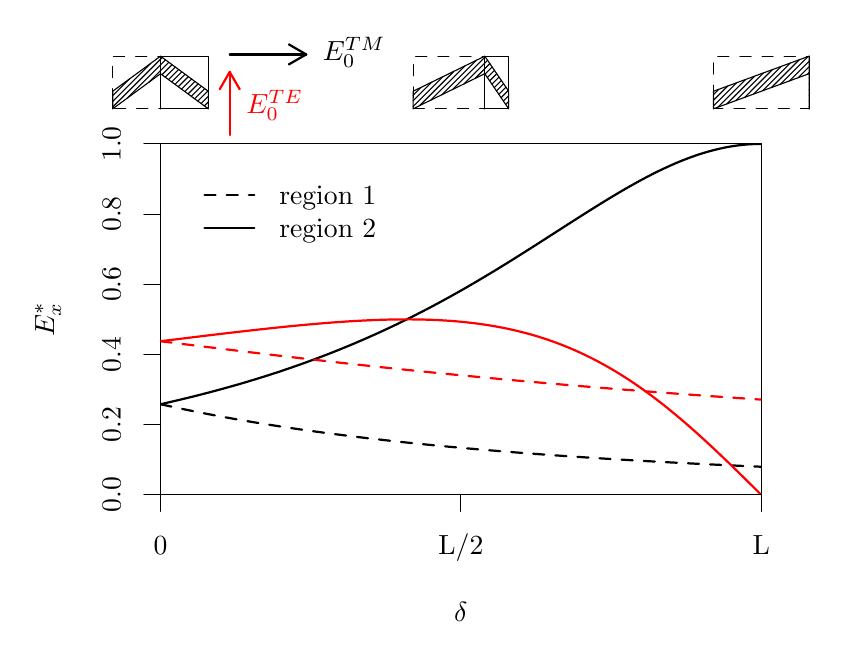
\begin{tikzpicture}[x=1pt,y=1pt]
\definecolor[named]{fillColor}{rgb}{1.00,1.00,1.00}
\path[use as bounding box,fill=fillColor,fill opacity=0.00] (0,0) rectangle (289.08,216.81);
\begin{scope}
\path[clip] ( 48.00, 48.00) rectangle (265.08,174.81);
\definecolor[named]{drawColor}{rgb}{0.00,0.00,0.00}

\path[draw=drawColor,line width= 0.8pt,dash pattern=on 4pt off 4pt ,line join=round,line cap=round] ( 48.00, 80.74) --
	( 50.19, 80.26) --
	( 52.39, 79.78) --
	( 54.58, 79.32) --
	( 56.77, 78.86) --
	( 58.96, 78.41) --
	( 61.16, 77.97) --
	( 63.35, 77.54) --
	( 65.54, 77.11) --
	( 67.73, 76.70) --
	( 69.93, 76.29) --
	( 72.12, 75.89) --
	( 74.31, 75.50) --
	( 76.51, 75.12) --
	( 78.70, 74.74) --
	( 80.89, 74.37) --
	( 83.08, 74.01) --
	( 85.28, 73.65) --
	( 87.47, 73.30) --
	( 89.66, 72.96) --
	( 91.85, 72.62) --
	( 94.05, 72.29) --
	( 96.24, 71.97) --
	( 98.43, 71.65) --
	(100.63, 71.33) --
	(102.82, 71.03) --
	(105.01, 70.73) --
	(107.20, 70.43) --
	(109.40, 70.14) --
	(111.59, 69.86) --
	(113.78, 69.58) --
	(115.97, 69.30) --
	(118.17, 69.03) --
	(120.36, 68.76) --
	(122.55, 68.50) --
	(124.75, 68.25) --
	(126.94, 68.00) --
	(129.13, 67.75) --
	(131.32, 67.51) --
	(133.52, 67.27) --
	(135.71, 67.03) --
	(137.90, 66.80) --
	(140.09, 66.57) --
	(142.29, 66.35) --
	(144.48, 66.13) --
	(146.67, 65.92) --
	(148.87, 65.70) --
	(151.06, 65.50) --
	(153.25, 65.29) --
	(155.44, 65.09) --
	(157.64, 64.89) --
	(159.83, 64.70) --
	(162.02, 64.51) --
	(164.21, 64.32) --
	(166.41, 64.13) --
	(168.60, 63.95) --
	(170.79, 63.77) --
	(172.99, 63.59) --
	(175.18, 63.42) --
	(177.37, 63.25) --
	(179.56, 63.08) --
	(181.76, 62.91) --
	(183.95, 62.75) --
	(186.14, 62.59) --
	(188.33, 62.43) --
	(190.53, 62.27) --
	(192.72, 62.12) --
	(194.91, 61.97) --
	(197.11, 61.82) --
	(199.30, 61.68) --
	(201.49, 61.53) --
	(203.68, 61.39) --
	(205.88, 61.25) --
	(208.07, 61.11) --
	(210.26, 60.98) --
	(212.45, 60.84) --
	(214.65, 60.71) --
	(216.84, 60.58) --
	(219.03, 60.45) --
	(221.23, 60.33) --
	(223.42, 60.20) --
	(225.61, 60.08) --
	(227.80, 59.96) --
	(230.00, 59.84) --
	(232.19, 59.72) --
	(234.38, 59.61) --
	(236.57, 59.50) --
	(238.77, 59.38) --
	(240.96, 59.27) --
	(243.15, 59.16) --
	(245.35, 59.06) --
	(247.54, 58.95) --
	(249.73, 58.85) --
	(251.92, 58.74) --
	(254.12, 58.64) --
	(256.31, 58.54) --
	(258.50, 58.44) --
	(260.69, 58.34) --
	(262.89, 58.25) --
	(265.08, 58.15);
\end{scope}
\begin{scope}
\path[clip] (  0.00,  0.00) rectangle (289.08,216.81);
\definecolor[named]{drawColor}{rgb}{0.00,0.00,0.00}

\path[draw=drawColor,line width= 0.4pt,line join=round,line cap=round] ( 48.00, 48.00) -- ( 48.00,174.81);

\path[draw=drawColor,line width= 0.4pt,line join=round,line cap=round] ( 48.00, 48.00) -- ( 42.00, 48.00);

\path[draw=drawColor,line width= 0.4pt,line join=round,line cap=round] ( 48.00, 73.36) -- ( 42.00, 73.36);

\path[draw=drawColor,line width= 0.4pt,line join=round,line cap=round] ( 48.00, 98.72) -- ( 42.00, 98.72);

\path[draw=drawColor,line width= 0.4pt,line join=round,line cap=round] ( 48.00,124.09) -- ( 42.00,124.09);

\path[draw=drawColor,line width= 0.4pt,line join=round,line cap=round] ( 48.00,149.45) -- ( 42.00,149.45);

\path[draw=drawColor,line width= 0.4pt,line join=round,line cap=round] ( 48.00,174.81) -- ( 42.00,174.81);

\node[text=drawColor,rotate= 90.00,anchor=base,inner sep=0pt, outer sep=0pt, scale=  1.00] at ( 33.60, 48.00) {0.0};

\node[text=drawColor,rotate= 90.00,anchor=base,inner sep=0pt, outer sep=0pt, scale=  1.00] at ( 33.60, 73.36) {0.2};

\node[text=drawColor,rotate= 90.00,anchor=base,inner sep=0pt, outer sep=0pt, scale=  1.00] at ( 33.60, 98.72) {0.4};

\node[text=drawColor,rotate= 90.00,anchor=base,inner sep=0pt, outer sep=0pt, scale=  1.00] at ( 33.60,124.09) {0.6};

\node[text=drawColor,rotate= 90.00,anchor=base,inner sep=0pt, outer sep=0pt, scale=  1.00] at ( 33.60,149.45) {0.8};

\node[text=drawColor,rotate= 90.00,anchor=base,inner sep=0pt, outer sep=0pt, scale=  1.00] at ( 33.60,174.81) {1.0};

\path[draw=drawColor,line width= 0.4pt,line join=round,line cap=round] ( 48.00, 48.00) --
	(265.08, 48.00) --
	(265.08,174.81) --
	( 48.00,174.81) --
	( 48.00, 48.00);
\end{scope}
\begin{scope}
\path[clip] (  0.00,  0.00) rectangle (289.08,216.81);
\definecolor[named]{drawColor}{rgb}{0.00,0.00,0.00}

\node[text=drawColor,anchor=base,inner sep=0pt, outer sep=0pt, scale=  1.00] at (156.54,  2.40) {$\delta$};

\node[text=drawColor,rotate= 90.00,anchor=base,inner sep=0pt, outer sep=0pt, scale=  1.00] at (  9.60,111.41) {$E_x^*$};
\end{scope}
\begin{scope}
\path[clip] ( 48.00, 48.00) rectangle (265.08,174.81);
\definecolor[named]{drawColor}{rgb}{0.00,0.00,0.00}

\path[draw=drawColor,line width= 0.8pt,line join=round,line cap=round] ( 48.00, 80.74) --
	( 50.19, 81.24) --
	( 52.39, 81.75) --
	( 54.58, 82.26) --
	( 56.77, 82.79) --
	( 58.96, 83.32) --
	( 61.16, 83.87) --
	( 63.35, 84.43) --
	( 65.54, 85.00) --
	( 67.73, 85.58) --
	( 69.93, 86.18) --
	( 72.12, 86.78) --
	( 74.31, 87.40) --
	( 76.51, 88.03) --
	( 78.70, 88.67) --
	( 80.89, 89.33) --
	( 83.08, 90.00) --
	( 85.28, 90.68) --
	( 87.47, 91.38) --
	( 89.66, 92.09) --
	( 91.85, 92.82) --
	( 94.05, 93.56) --
	( 96.24, 94.32) --
	( 98.43, 95.09) --
	(100.63, 95.88) --
	(102.82, 96.68) --
	(105.01, 97.50) --
	(107.20, 98.33) --
	(109.40, 99.18) --
	(111.59,100.05) --
	(113.78,100.94) --
	(115.97,101.84) --
	(118.17,102.76) --
	(120.36,103.70) --
	(122.55,104.65) --
	(124.75,105.63) --
	(126.94,106.62) --
	(129.13,107.63) --
	(131.32,108.66) --
	(133.52,109.70) --
	(135.71,110.77) --
	(137.90,111.85) --
	(140.09,112.95) --
	(142.29,114.08) --
	(144.48,115.21) --
	(146.67,116.37) --
	(148.87,117.55) --
	(151.06,118.74) --
	(153.25,119.95) --
	(155.44,121.18) --
	(157.64,122.43) --
	(159.83,123.69) --
	(162.02,124.97) --
	(164.21,126.27) --
	(166.41,127.58) --
	(168.60,128.90) --
	(170.79,130.24) --
	(172.99,131.59) --
	(175.18,132.95) --
	(177.37,134.33) --
	(179.56,135.71) --
	(181.76,137.10) --
	(183.95,138.50) --
	(186.14,139.90) --
	(188.33,141.31) --
	(190.53,142.72) --
	(192.72,144.13) --
	(194.91,145.54) --
	(197.11,146.94) --
	(199.30,148.34) --
	(201.49,149.73) --
	(203.68,151.11) --
	(205.88,152.48) --
	(208.07,153.84) --
	(210.26,155.18) --
	(212.45,156.49) --
	(214.65,157.79) --
	(216.84,159.06) --
	(219.03,160.29) --
	(221.23,161.50) --
	(223.42,162.68) --
	(225.61,163.81) --
	(227.80,164.91) --
	(230.00,165.96) --
	(232.19,166.96) --
	(234.38,167.92) --
	(236.57,168.82) --
	(238.77,169.67) --
	(240.96,170.47) --
	(243.15,171.20) --
	(245.35,171.87) --
	(247.54,172.47) --
	(249.73,173.01) --
	(251.92,173.49) --
	(254.12,173.89) --
	(256.31,174.22) --
	(258.50,174.48) --
	(260.69,174.66) --
	(262.89,174.77) --
	(265.08,174.81);
\definecolor[named]{drawColor}{rgb}{1.00,0.00,0.00}

\path[draw=drawColor,line width= 0.8pt,dash pattern=on 4pt off 4pt ,line join=round,line cap=round] ( 48.00,103.50) --
	( 50.19,103.23) --
	( 52.39,102.96) --
	( 54.58,102.68) --
	( 56.77,102.41) --
	( 58.96,102.14) --
	( 61.16,101.87) --
	( 63.35,101.60) --
	( 65.54,101.33) --
	( 67.73,101.06) --
	( 69.93,100.79) --
	( 72.12,100.53) --
	( 74.31,100.26) --
	( 76.51, 99.99) --
	( 78.70, 99.73) --
	( 80.89, 99.46) --
	( 83.08, 99.20) --
	( 85.28, 98.94) --
	( 87.47, 98.68) --
	( 89.66, 98.42) --
	( 91.85, 98.16) --
	( 94.05, 97.90) --
	( 96.24, 97.65) --
	( 98.43, 97.39) --
	(100.63, 97.14) --
	(102.82, 96.89) --
	(105.01, 96.64) --
	(107.20, 96.39) --
	(109.40, 96.14) --
	(111.59, 95.89) --
	(113.78, 95.65) --
	(115.97, 95.41) --
	(118.17, 95.17) --
	(120.36, 94.93) --
	(122.55, 94.69) --
	(124.75, 94.45) --
	(126.94, 94.21) --
	(129.13, 93.98) --
	(131.32, 93.75) --
	(133.52, 93.52) --
	(135.71, 93.29) --
	(137.90, 93.06) --
	(140.09, 92.84) --
	(142.29, 92.61) --
	(144.48, 92.39) --
	(146.67, 92.17) --
	(148.87, 91.95) --
	(151.06, 91.73) --
	(153.25, 91.52) --
	(155.44, 91.30) --
	(157.64, 91.09) --
	(159.83, 90.88) --
	(162.02, 90.67) --
	(164.21, 90.46) --
	(166.41, 90.25) --
	(168.60, 90.05) --
	(170.79, 89.84) --
	(172.99, 89.64) --
	(175.18, 89.44) --
	(177.37, 89.24) --
	(179.56, 89.05) --
	(181.76, 88.85) --
	(183.95, 88.66) --
	(186.14, 88.46) --
	(188.33, 88.27) --
	(190.53, 88.08) --
	(192.72, 87.89) --
	(194.91, 87.70) --
	(197.11, 87.52) --
	(199.30, 87.33) --
	(201.49, 87.15) --
	(203.68, 86.97) --
	(205.88, 86.79) --
	(208.07, 86.61) --
	(210.26, 86.43) --
	(212.45, 86.26) --
	(214.65, 86.08) --
	(216.84, 85.91) --
	(219.03, 85.74) --
	(221.23, 85.57) --
	(223.42, 85.40) --
	(225.61, 85.23) --
	(227.80, 85.06) --
	(230.00, 84.90) --
	(232.19, 84.73) --
	(234.38, 84.57) --
	(236.57, 84.41) --
	(238.77, 84.25) --
	(240.96, 84.09) --
	(243.15, 83.93) --
	(245.35, 83.77) --
	(247.54, 83.62) --
	(249.73, 83.46) --
	(251.92, 83.31) --
	(254.12, 83.16) --
	(256.31, 83.01) --
	(258.50, 82.86) --
	(260.69, 82.71) --
	(262.89, 82.56) --
	(265.08, 82.41);

\path[draw=drawColor,line width= 0.8pt,line join=round,line cap=round] ( 48.00,103.50) --
	( 50.19,103.77) --
	( 52.39,104.04) --
	( 54.58,104.31) --
	( 56.77,104.58) --
	( 58.96,104.85) --
	( 61.16,105.11) --
	( 63.35,105.38) --
	( 65.54,105.65) --
	( 67.73,105.91) --
	( 69.93,106.17) --
	( 72.12,106.43) --
	( 74.31,106.69) --
	( 76.51,106.94) --
	( 78.70,107.19) --
	( 80.89,107.44) --
	( 83.08,107.68) --
	( 85.28,107.92) --
	( 87.47,108.16) --
	( 89.66,108.39) --
	( 91.85,108.62) --
	( 94.05,108.84) --
	( 96.24,109.06) --
	( 98.43,109.27) --
	(100.63,109.47) --
	(102.82,109.67) --
	(105.01,109.86) --
	(107.20,110.04) --
	(109.40,110.22) --
	(111.59,110.38) --
	(113.78,110.53) --
	(115.97,110.68) --
	(118.17,110.81) --
	(120.36,110.93) --
	(122.55,111.04) --
	(124.75,111.14) --
	(126.94,111.22) --
	(129.13,111.29) --
	(131.32,111.35) --
	(133.52,111.38) --
	(135.71,111.40) --
	(137.90,111.40) --
	(140.09,111.39) --
	(142.29,111.35) --
	(144.48,111.29) --
	(146.67,111.21) --
	(148.87,111.11) --
	(151.06,110.98) --
	(153.25,110.83) --
	(155.44,110.65) --
	(157.64,110.44) --
	(159.83,110.20) --
	(162.02,109.94) --
	(164.21,109.64) --
	(166.41,109.31) --
	(168.60,108.94) --
	(170.79,108.54) --
	(172.99,108.11) --
	(175.18,107.63) --
	(177.37,107.12) --
	(179.56,106.56) --
	(181.76,105.97) --
	(183.95,105.33) --
	(186.14,104.64) --
	(188.33,103.91) --
	(190.53,103.13) --
	(192.72,102.31) --
	(194.91,101.43) --
	(197.11,100.51) --
	(199.30, 99.54) --
	(201.49, 98.51) --
	(203.68, 97.43) --
	(205.88, 96.30) --
	(208.07, 95.11) --
	(210.26, 93.87) --
	(212.45, 92.58) --
	(214.65, 91.23) --
	(216.84, 89.83) --
	(219.03, 88.37) --
	(221.23, 86.86) --
	(223.42, 85.30) --
	(225.61, 83.69) --
	(227.80, 82.03) --
	(230.00, 80.31) --
	(232.19, 78.55) --
	(234.38, 76.74) --
	(236.57, 74.89) --
	(238.77, 73.00) --
	(240.96, 71.06) --
	(243.15, 69.09) --
	(245.35, 67.09) --
	(247.54, 65.05) --
	(249.73, 62.98) --
	(251.92, 60.89) --
	(254.12, 58.78) --
	(256.31, 56.64) --
	(258.50, 54.50) --
	(260.69, 52.34) --
	(262.89, 50.17) --
	(265.08, 48.00);
\end{scope}
\begin{scope}
\path[clip] (  0.00,  0.00) rectangle (289.08,216.81);
\definecolor[named]{drawColor}{rgb}{0.00,0.00,0.00}

\path[draw=drawColor,line width= 0.4pt,line join=round,line cap=round] ( 48.00, 48.00) -- (265.08, 48.00);

\path[draw=drawColor,line width= 0.4pt,line join=round,line cap=round] ( 48.00, 48.00) -- ( 48.00, 42.00);

\path[draw=drawColor,line width= 0.4pt,line join=round,line cap=round] (156.54, 48.00) -- (156.54, 42.00);

\path[draw=drawColor,line width= 0.4pt,line join=round,line cap=round] (265.08, 48.00) -- (265.08, 42.00);

\node[text=drawColor,anchor=base,inner sep=0pt, outer sep=0pt, scale=  1.00] at ( 48.00, 26.40) {0};

\node[text=drawColor,anchor=base,inner sep=0pt, outer sep=0pt, scale=  1.00] at (156.54, 26.40) {L/2};

\node[text=drawColor,anchor=base,inner sep=0pt, outer sep=0pt, scale=  1.00] at (265.08, 26.40) {L};
\end{scope}
\begin{scope}
\path[clip] (  0.00,  0.00) rectangle (289.08,216.81);
\definecolor[named]{drawColor}{rgb}{0.00,0.00,0.00}

\path[draw=drawColor,line width= 0.4pt,line join=round,line cap=round] ( 30.73,192.21) -- ( 36.82,198.31);

\path[draw=drawColor,line width= 0.4pt,line join=round,line cap=round] ( 30.73,190.17) -- ( 44.51,203.95);

\path[draw=drawColor,line width= 0.4pt,line join=round,line cap=round] ( 30.73,188.12) -- ( 48.64,206.04);

\path[draw=drawColor,line width= 0.4pt,line join=round,line cap=round] ( 36.04,191.39) -- ( 49.82,205.17);

\path[draw=drawColor,line width= 0.4pt,line join=round,line cap=round] ( 43.73,197.04) -- ( 51.00,204.31);

\path[draw=drawColor,line width= 0.4pt,line join=round,line cap=round] ( 48.52,199.79) -- ( 52.18,203.44);

\path[draw=drawColor,line width= 0.4pt,line join=round,line cap=round] ( 49.70,198.92) -- ( 53.36,202.58);

\path[draw=drawColor,line width= 0.4pt,line join=round,line cap=round] ( 50.88,198.06) -- ( 54.54,201.71);

\path[draw=drawColor,line width= 0.4pt,line join=round,line cap=round] ( 52.06,197.19) -- ( 55.72,200.85);

\path[draw=drawColor,line width= 0.4pt,line join=round,line cap=round] ( 53.24,196.33) -- ( 56.90,199.98);

\path[draw=drawColor,line width= 0.4pt,line join=round,line cap=round] ( 54.42,195.46) -- ( 58.07,199.12);

\path[draw=drawColor,line width= 0.4pt,line join=round,line cap=round] ( 55.60,194.60) -- ( 59.25,198.25);

\path[draw=drawColor,line width= 0.4pt,line join=round,line cap=round] ( 56.78,193.73) -- ( 60.43,197.39);

\path[draw=drawColor,line width= 0.4pt,line join=round,line cap=round] ( 57.95,192.86) -- ( 61.61,196.52);

\path[draw=drawColor,line width= 0.4pt,line join=round,line cap=round] ( 59.13,192.00) -- ( 62.79,195.66);

\path[draw=drawColor,line width= 0.4pt,line join=round,line cap=round] ( 60.31,191.13) -- ( 63.97,194.79);

\path[draw=drawColor,line width= 0.4pt,line join=round,line cap=round] ( 61.49,190.27) -- ( 65.15,193.93);

\path[draw=drawColor,line width= 0.4pt,line join=round,line cap=round] ( 62.67,189.40) -- ( 65.27,192.01);

\path[draw=drawColor,line width= 0.4pt,line join=round,line cap=round] ( 63.85,188.54) -- ( 65.27,189.97);

\path[draw=drawColor,line width= 0.4pt,line join=round,line cap=round] ( 65.03,187.67) -- ( 65.27,187.92);

\path[draw=drawColor,line width= 0.4pt,line join=round,line cap=round] ( 30.73,193.83) --
	( 48.00,206.51) --
	( 65.27,193.83) --
	( 65.27,187.49) --
	( 48.00,200.17) --
	( 30.73,187.49) --
	( 30.73,193.83);

\path[draw=drawColor,line width= 0.4pt,line join=round,line cap=round] ( 48.00,187.49) --
	( 48.00,206.51) --
	( 65.27,206.51) --
	( 65.27,187.49) --
	( 48.00,187.49);

\path[draw=drawColor,line width= 0.4pt,dash pattern=on 4pt off 4pt ,line join=round,line cap=round] ( 48.00,187.49) --
	( 48.00,206.51) --
	( 30.73,206.51) --
	( 30.73,187.49) --
	( 48.00,187.49);

\path[draw=drawColor,line width= 0.4pt,line join=round,line cap=round] (247.81,192.61) -- (249.73,194.54);

\path[draw=drawColor,line width= 0.4pt,line join=round,line cap=round] (247.81,190.57) -- (252.96,195.72);

\path[draw=drawColor,line width= 0.4pt,line join=round,line cap=round] (247.81,188.53) -- (256.19,196.91);

\path[draw=drawColor,line width= 0.4pt,line join=round,line cap=round] (249.40,188.08) -- (259.42,198.09);

\path[draw=drawColor,line width= 0.4pt,line join=round,line cap=round] (252.63,189.26) -- (262.65,199.28);

\path[draw=drawColor,line width= 0.4pt,line join=round,line cap=round] (255.86,190.45) -- (265.88,200.46);

\path[draw=drawColor,line width= 0.4pt,line join=round,line cap=round] (259.09,191.63) -- (269.10,201.65);

\path[draw=drawColor,line width= 0.4pt,line join=round,line cap=round] (262.32,192.82) -- (272.33,202.83);

\path[draw=drawColor,line width= 0.4pt,line join=round,line cap=round] (265.55,194.00) -- (275.56,204.02);

\path[draw=drawColor,line width= 0.4pt,line join=round,line cap=round] (268.78,195.19) -- (278.79,205.21);

\path[draw=drawColor,line width= 0.4pt,line join=round,line cap=round] (272.01,196.37) -- (282.02,206.39);

\path[draw=drawColor,line width= 0.4pt,line join=round,line cap=round] (275.23,197.56) -- (282.35,204.68);

\path[draw=drawColor,line width= 0.4pt,line join=round,line cap=round] (278.46,198.74) -- (282.35,202.63);

\path[draw=drawColor,line width= 0.4pt,line join=round,line cap=round] (281.69,199.93) -- (282.35,200.59);

\path[draw=drawColor,line width= 0.4pt,line join=round,line cap=round] (282.35,198.55) -- (282.35,198.55);

\path[draw=drawColor,line width= 0.4pt,line join=round,line cap=round] (282.35,196.50) -- (282.35,196.50);

\path[draw=drawColor,line width= 0.4pt,line join=round,line cap=round] (282.35,194.46) -- (282.35,194.46);

\path[draw=drawColor,line width= 0.4pt,line join=round,line cap=round] (282.35,192.41) -- (282.35,192.41);

\path[draw=drawColor,line width= 0.4pt,line join=round,line cap=round] (282.35,190.37) -- (282.35,190.37);

\path[draw=drawColor,line width= 0.4pt,line join=round,line cap=round] (282.35,188.33) -- (282.35,188.33);

\path[draw=drawColor,line width= 0.4pt,line join=round,line cap=round] (247.81,193.83) --
	(282.35,206.51) --
	(282.35,193.83) --
	(282.35,187.49) --
	(282.35,200.17) --
	(247.81,187.49) --
	(247.81,193.83);

\path[draw=drawColor,line width= 0.4pt,line join=round,line cap=round] (282.35,187.49) --
	(282.35,206.51) --
	(282.35,206.51) --
	(282.35,187.49) --
	(282.35,187.49);

\path[draw=drawColor,line width= 0.4pt,dash pattern=on 4pt off 4pt ,line join=round,line cap=round] (282.35,187.49) --
	(282.35,206.51) --
	(247.81,206.51) --
	(247.81,187.49) --
	(282.35,187.49);

\path[draw=drawColor,line width= 0.4pt,line join=round,line cap=round] (139.27,192.41) -- (142.05,195.19);

\path[draw=drawColor,line width= 0.4pt,line join=round,line cap=round] (139.27,190.37) -- (146.05,197.15);

\path[draw=drawColor,line width= 0.4pt,line join=round,line cap=round] (139.27,188.32) -- (150.05,199.11);

\path[draw=drawColor,line width= 0.4pt,line join=round,line cap=round] (141.64,188.65) -- (154.05,201.07);

\path[draw=drawColor,line width= 0.4pt,line join=round,line cap=round] (145.64,190.61) -- (158.06,203.03);

\path[draw=drawColor,line width= 0.4pt,line join=round,line cap=round] (149.64,192.57) -- (162.06,204.99);

\path[draw=drawColor,line width= 0.4pt,line join=round,line cap=round] (153.65,194.53) -- (165.36,206.24);

\path[draw=drawColor,line width= 0.4pt,line join=round,line cap=round] (157.65,196.49) -- (166.19,205.03);

\path[draw=drawColor,line width= 0.4pt,line join=round,line cap=round] (161.65,198.45) -- (167.02,203.81);

\path[draw=drawColor,line width= 0.4pt,line join=round,line cap=round] (165.28,200.03) -- (167.85,202.60);

\path[draw=drawColor,line width= 0.4pt,line join=round,line cap=round] (166.10,198.81) -- (168.67,201.38);

\path[draw=drawColor,line width= 0.4pt,line join=round,line cap=round] (166.93,197.59) -- (169.50,200.16);

\path[draw=drawColor,line width= 0.4pt,line join=round,line cap=round] (167.76,196.38) -- (170.33,198.95);

\path[draw=drawColor,line width= 0.4pt,line join=round,line cap=round] (168.59,195.16) -- (171.16,197.73);

\path[draw=drawColor,line width= 0.4pt,line join=round,line cap=round] (169.42,193.95) -- (171.99,196.52);

\path[draw=drawColor,line width= 0.4pt,line join=round,line cap=round] (170.25,192.73) -- (172.81,195.30);

\path[draw=drawColor,line width= 0.4pt,line join=round,line cap=round] (171.07,191.51) -- (173.64,194.08);

\path[draw=drawColor,line width= 0.4pt,line join=round,line cap=round] (171.90,190.30) -- (173.81,192.21);

\path[draw=drawColor,line width= 0.4pt,line join=round,line cap=round] (172.73,189.08) -- (173.81,190.17);

\path[draw=drawColor,line width= 0.4pt,line join=round,line cap=round] (173.56,187.87) -- (173.81,188.12);

\path[draw=drawColor,line width= 0.4pt,line join=round,line cap=round] (139.27,193.83) --
	(165.18,206.51) --
	(173.81,193.83) --
	(173.81,187.49) --
	(165.18,200.17) --
	(139.27,187.49) --
	(139.27,193.83);

\path[draw=drawColor,line width= 0.4pt,line join=round,line cap=round] (165.18,187.49) --
	(165.18,206.51) --
	(173.81,206.51) --
	(173.81,187.49) --
	(165.18,187.49);

\path[draw=drawColor,line width= 0.4pt,dash pattern=on 4pt off 4pt ,line join=round,line cap=round] (165.18,187.49) --
	(165.18,206.51) --
	(139.27,206.51) --
	(139.27,187.49) --
	(165.18,187.49);

\path[draw=drawColor,line width= 0.8pt,line join=round,line cap=round] ( 73.00,207.15) -- (100.64,207.15);

\path[draw=drawColor,line width= 0.8pt,line join=round,line cap=round] ( 94.38,203.53) --
	(100.64,207.15) --
	( 94.38,210.76);

\node[text=drawColor,anchor=base west,inner sep=0pt, outer sep=0pt, scale=  1.00] at (106.64,204.85) {$E_0^{TM}$};
\definecolor[named]{drawColor}{rgb}{1.00,0.00,0.00}

\path[draw=drawColor,line width= 0.8pt,line join=round,line cap=round] ( 73.00,177.98) -- ( 73.00,200.81);

\path[draw=drawColor,line width= 0.8pt,line join=round,line cap=round] ( 76.61,194.55) --
	( 73.00,200.81) --
	( 69.39,194.55);

\node[text=drawColor,anchor=base west,inner sep=0pt, outer sep=0pt, scale=  1.00] at ( 79.00,185.83) {$E_0^{TE}$};

\path[] ( 54.91,168.47) rectangle (130.43,132.47);
\definecolor[named]{drawColor}{rgb}{0.00,0.00,0.00}

\path[draw=drawColor,line width= 0.8pt,dash pattern=on 4pt off 4pt ,line join=round,line cap=round] ( 63.91,156.47) -- ( 81.91,156.47);

\path[draw=drawColor,line width= 0.8pt,line join=round,line cap=round] ( 63.91,144.47) -- ( 81.91,144.47);

\node[text=drawColor,anchor=base west,inner sep=0pt, outer sep=0pt, scale=  1.00] at ( 90.91,153.03) {region 1};

\node[text=drawColor,anchor=base west,inner sep=0pt, outer sep=0pt, scale=  1.00] at ( 90.91,141.03) {region 2};
\end{scope}
\end{tikzpicture}

\end{center}
\caption[Magnitude of the electric field in region 1 and region 2, for the two polarisation cases of TM and TE polarised light.]{Magnitude of the electric field in region 1 (dashed) and region 2 (dotted) for the two polarisation cases of TM (black) and TE (red) polarised light, as a function of offset, $\delta$.  \label{fig:as-maxEwithdelta}}
\end{figure}

We may now expand these two functions as a Fourier sum to determine which diffracted SPP wavevectors may be matched with incident plane waves for each polarisation case. We do this for an asymmetric zigzag grating with $\delta=0.42L=126\:\nano\metre$ the offset which was measured from the SEMs of the produced sample. Since the $E_{x}^{TE}$ and $E_{x}^{TM}$ functions are neither odd nor even, we expand them as a complex Fourier sum, and the take the magnitude of the Fourier components squared to obtain a qualitative understanding of the relative scattering efficiencies \cite{Goodman2005}. The complex Fourier series coefficients are given by,
\begin{equation}
C_n=\frac{1}{L} \int_{-L}^L \! f(x)\exp{(-inx)} \, \mathrm{d} x
\end{equation}
Where $n$ is the order of the Fourier harmonic. The Fourier components for both $E_x^{TE}$ and $E_x^{TM}$ functions are plotted in figure \ref{fig:as-fouriers}. The efficiency with which light will couple to the SPPs on an asymmetric zigzag grating will be directly linked to the amplitudes of these Fourier coefficients, as the strength of each harmonic equates to the scattering amplitude of the SPPs. These coefficients are different for each polarisation, but they will not be zero. 
\begin{figure}
\begin{center}
\subfigure[TE]{\input{figure-azz-fourier-coeffs-TE.tex}}
\subfigure[TM]{% Created by tikzDevice version 0.6.2-92-0ad2792 on 2013-02-01 15:13:44
% !TEX encoding = UTF-8 Unicode
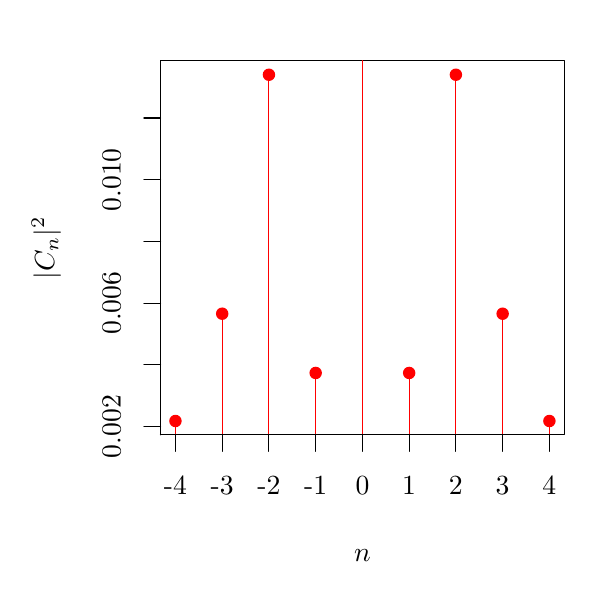
\begin{tikzpicture}[x=1pt,y=1pt]
\definecolor[named]{fillColor}{rgb}{1.00,1.00,1.00}
\path[use as bounding box,fill=fillColor,fill opacity=0.00] (0,0) rectangle (195.13,195.13);
\begin{scope}
\path[clip] ( 48.00, 48.00) rectangle (193.93,183.13);
\definecolor[named]{fillColor}{rgb}{1.00,0.00,0.00}

\path[fill=fillColor] (104.07, 70.36) circle (  2.25);

\path[fill=fillColor] ( 87.18,178.12) circle (  2.25);

\path[fill=fillColor] ( 70.29, 91.77) circle (  2.25);

\path[fill=fillColor] ( 53.40, 53.00) circle (  2.25);

\path[fill=fillColor] (137.85, 70.36) circle (  2.25);

\path[fill=fillColor] (154.74,178.12) circle (  2.25);

\path[fill=fillColor] (171.63, 91.77) circle (  2.25);

\path[fill=fillColor] (188.52, 53.00) circle (  2.25);
\end{scope}
\begin{scope}
\path[clip] (  0.00,  0.00) rectangle (195.13,195.13);
\definecolor[named]{drawColor}{rgb}{0.00,0.00,0.00}

\path[draw=drawColor,line width= 0.4pt,line join=round,line cap=round] ( 48.00, 50.99) -- ( 48.00,162.49);

\path[draw=drawColor,line width= 0.4pt,line join=round,line cap=round] ( 48.00, 50.99) -- ( 42.00, 50.99);

\path[draw=drawColor,line width= 0.4pt,line join=round,line cap=round] ( 48.00, 73.29) -- ( 42.00, 73.29);

\path[draw=drawColor,line width= 0.4pt,line join=round,line cap=round] ( 48.00, 95.59) -- ( 42.00, 95.59);

\path[draw=drawColor,line width= 0.4pt,line join=round,line cap=round] ( 48.00,117.89) -- ( 42.00,117.89);

\path[draw=drawColor,line width= 0.4pt,line join=round,line cap=round] ( 48.00,140.19) -- ( 42.00,140.19);

\path[draw=drawColor,line width= 0.4pt,line join=round,line cap=round] ( 48.00,162.49) -- ( 42.00,162.49);

\node[text=drawColor,rotate= 90.00,anchor=base,inner sep=0pt, outer sep=0pt, scale=  1.00] at ( 33.60, 50.99) {0.002};

\node[text=drawColor,rotate= 90.00,anchor=base,inner sep=0pt, outer sep=0pt, scale=  1.00] at ( 33.60, 95.59) {0.006};

\node[text=drawColor,rotate= 90.00,anchor=base,inner sep=0pt, outer sep=0pt, scale=  1.00] at ( 33.60,140.19) {0.010};

\path[draw=drawColor,line width= 0.4pt,line join=round,line cap=round] ( 48.00, 48.00) --
	(193.93, 48.00) --
	(193.93,183.13) --
	( 48.00,183.13) --
	( 48.00, 48.00);
\end{scope}
\begin{scope}
\path[clip] (  0.00,  0.00) rectangle (195.13,195.13);
\definecolor[named]{drawColor}{rgb}{0.00,0.00,0.00}

\node[text=drawColor,anchor=base,inner sep=0pt, outer sep=0pt, scale=  1.00] at (120.96,  2.40) {$n$};

\node[text=drawColor,rotate= 90.00,anchor=base,inner sep=0pt, outer sep=0pt, scale=  1.00] at (  9.60,115.56) {$|C_n|^2$};
\end{scope}
\begin{scope}
\path[clip] ( 48.00, 48.00) rectangle (193.93,183.13);
\definecolor[named]{drawColor}{rgb}{1.00,0.00,0.00}

\path[draw=drawColor,line width= 0.4pt,line join=round,line cap=round] (137.85, 28.70) --
	(137.85, 70.36);

\path[draw=drawColor,line width= 0.4pt,line join=round,line cap=round] (154.74, 28.70) --
	(154.74,178.12);

\path[draw=drawColor,line width= 0.4pt,line join=round,line cap=round] (171.63, 28.70) --
	(171.63, 91.77);

\path[draw=drawColor,line width= 0.4pt,line join=round,line cap=round] (188.52, 28.70) --
	(188.52, 53.00);

\path[draw=drawColor,line width= 0.4pt,line join=round,line cap=round] (104.07, 28.70) --
	(104.07, 70.36);

\path[draw=drawColor,line width= 0.4pt,line join=round,line cap=round] ( 87.18, 28.70) --
	( 87.18,178.12);

\path[draw=drawColor,line width= 0.4pt,line join=round,line cap=round] ( 70.29, 28.70) --
	( 70.29, 91.77);

\path[draw=drawColor,line width= 0.4pt,line join=round,line cap=round] ( 53.40, 28.70) --
	( 53.40, 53.00);

\path[draw=drawColor,line width= 0.4pt,line join=round,line cap=round] (120.96, 28.70) --
	(120.96,195.13);
\end{scope}
\begin{scope}
\path[clip] (  0.00,  0.00) rectangle (195.13,195.13);
\definecolor[named]{drawColor}{rgb}{0.00,0.00,0.00}

\path[draw=drawColor,line width= 0.4pt,line join=round,line cap=round] ( 53.40, 48.00) -- (188.52, 48.00);

\path[draw=drawColor,line width= 0.4pt,line join=round,line cap=round] ( 53.40, 48.00) -- ( 53.40, 42.00);

\path[draw=drawColor,line width= 0.4pt,line join=round,line cap=round] ( 70.29, 48.00) -- ( 70.29, 42.00);

\path[draw=drawColor,line width= 0.4pt,line join=round,line cap=round] ( 87.18, 48.00) -- ( 87.18, 42.00);

\path[draw=drawColor,line width= 0.4pt,line join=round,line cap=round] (104.07, 48.00) -- (104.07, 42.00);

\path[draw=drawColor,line width= 0.4pt,line join=round,line cap=round] (120.96, 48.00) -- (120.96, 42.00);

\path[draw=drawColor,line width= 0.4pt,line join=round,line cap=round] (137.85, 48.00) -- (137.85, 42.00);

\path[draw=drawColor,line width= 0.4pt,line join=round,line cap=round] (154.74, 48.00) -- (154.74, 42.00);

\path[draw=drawColor,line width= 0.4pt,line join=round,line cap=round] (171.63, 48.00) -- (171.63, 42.00);

\path[draw=drawColor,line width= 0.4pt,line join=round,line cap=round] (188.52, 48.00) -- (188.52, 42.00);

\node[text=drawColor,anchor=base,inner sep=0pt, outer sep=0pt, scale=  1.00] at ( 53.40, 26.40) {-4};

\node[text=drawColor,anchor=base,inner sep=0pt, outer sep=0pt, scale=  1.00] at ( 70.29, 26.40) {-3};

\node[text=drawColor,anchor=base,inner sep=0pt, outer sep=0pt, scale=  1.00] at ( 87.18, 26.40) {-2};

\node[text=drawColor,anchor=base,inner sep=0pt, outer sep=0pt, scale=  1.00] at (104.07, 26.40) {-1};

\node[text=drawColor,anchor=base,inner sep=0pt, outer sep=0pt, scale=  1.00] at (120.96, 26.40) {0};

\node[text=drawColor,anchor=base,inner sep=0pt, outer sep=0pt, scale=  1.00] at (137.85, 26.40) {1};

\node[text=drawColor,anchor=base,inner sep=0pt, outer sep=0pt, scale=  1.00] at (154.74, 26.40) {2};

\node[text=drawColor,anchor=base,inner sep=0pt, outer sep=0pt, scale=  1.00] at (171.63, 26.40) {3};

\node[text=drawColor,anchor=base,inner sep=0pt, outer sep=0pt, scale=  1.00] at (188.52, 26.40) {4};
\end{scope}
\end{tikzpicture}
}
\end{center}
\caption[The square magnitude of the Fourier coefficients for $n=0...\pm 4$ with an offset of $\delta=0.42L$.]{The square magnitude of the Fourier coefficients for $n=0...\pm 4$ with an offset of $\delta=0.42L$, which corresponds to the experimentally measured offset of $126 \pm 5 \:\nano\metre$ for the (a) TE case and (b) TM case. \label{fig:as-fouriers}}
\end{figure}

This leads to the conclusion that both TE and TM polarised light will couple to all orders of SPPs on such a grating, with different (but non-zero) coupling strength depending on the diffracted order used to couple to the SPP. It is possible to excite any diffracted SPP mode with any polarisation of light on such a grating. That is to say, the same SPP mode may be driven with either polarisation.

Incidentally, examining the Fourier coefficients for no offset (setting $\delta=0$), we recover the polarisation selectivity predicted in chapter \ref{c:zigzag} for a symmetric zigzag grating. 

\subsection{Results}
The coupling of light to SPPs on an asymmetric zigzag grating is demonstrated experimentally in figure \ref{fig:azz-teandtmR}.
\begin{figure}
\begin{center}
% Created by tikzDevice version 0.6.2-92-0ad2792 on 2012-12-11 16:31:32
% !TEX encoding = UTF-8 Unicode
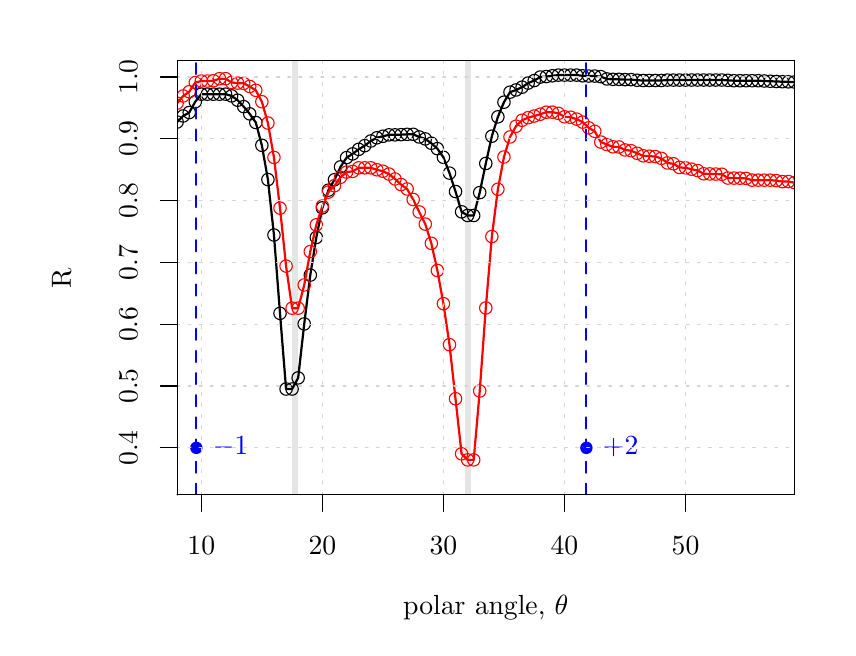
\begin{tikzpicture}[x=1pt,y=1pt]
\definecolor[named]{fillColor}{rgb}{1.00,1.00,1.00}
\path[use as bounding box,fill=fillColor,fill opacity=0.00] (0,0) rectangle (289.08,216.81);
\begin{scope}
\path[clip] (  0.00,  0.00) rectangle (289.08,216.81);
\definecolor[named]{drawColor}{rgb}{0.00,0.00,0.00}

\path[draw=drawColor,line width= 0.4pt,line join=round,line cap=round] ( 62.75, 48.00) -- (237.71, 48.00);

\path[draw=drawColor,line width= 0.4pt,line join=round,line cap=round] ( 62.75, 48.00) -- ( 62.75, 42.00);

\path[draw=drawColor,line width= 0.4pt,line join=round,line cap=round] (106.49, 48.00) -- (106.49, 42.00);

\path[draw=drawColor,line width= 0.4pt,line join=round,line cap=round] (150.23, 48.00) -- (150.23, 42.00);

\path[draw=drawColor,line width= 0.4pt,line join=round,line cap=round] (193.97, 48.00) -- (193.97, 42.00);

\path[draw=drawColor,line width= 0.4pt,line join=round,line cap=round] (237.71, 48.00) -- (237.71, 42.00);

\node[text=drawColor,anchor=base,inner sep=0pt, outer sep=0pt, scale=  1.00] at ( 62.75, 26.40) {10};

\node[text=drawColor,anchor=base,inner sep=0pt, outer sep=0pt, scale=  1.00] at (106.49, 26.40) {20};

\node[text=drawColor,anchor=base,inner sep=0pt, outer sep=0pt, scale=  1.00] at (150.23, 26.40) {30};

\node[text=drawColor,anchor=base,inner sep=0pt, outer sep=0pt, scale=  1.00] at (193.97, 26.40) {40};

\node[text=drawColor,anchor=base,inner sep=0pt, outer sep=0pt, scale=  1.00] at (237.71, 26.40) {50};

\path[draw=drawColor,line width= 0.4pt,line join=round,line cap=round] ( 54.00, 64.98) -- ( 54.00,199.00);

\path[draw=drawColor,line width= 0.4pt,line join=round,line cap=round] ( 54.00, 64.98) -- ( 48.00, 64.98);

\path[draw=drawColor,line width= 0.4pt,line join=round,line cap=round] ( 54.00, 87.31) -- ( 48.00, 87.31);

\path[draw=drawColor,line width= 0.4pt,line join=round,line cap=round] ( 54.00,109.65) -- ( 48.00,109.65);

\path[draw=drawColor,line width= 0.4pt,line join=round,line cap=round] ( 54.00,131.99) -- ( 48.00,131.99);

\path[draw=drawColor,line width= 0.4pt,line join=round,line cap=round] ( 54.00,154.33) -- ( 48.00,154.33);

\path[draw=drawColor,line width= 0.4pt,line join=round,line cap=round] ( 54.00,176.66) -- ( 48.00,176.66);

\path[draw=drawColor,line width= 0.4pt,line join=round,line cap=round] ( 54.00,199.00) -- ( 48.00,199.00);

\node[text=drawColor,rotate= 90.00,anchor=base,inner sep=0pt, outer sep=0pt, scale=  1.00] at ( 39.60, 64.98) {0.4};

\node[text=drawColor,rotate= 90.00,anchor=base,inner sep=0pt, outer sep=0pt, scale=  1.00] at ( 39.60, 87.31) {0.5};

\node[text=drawColor,rotate= 90.00,anchor=base,inner sep=0pt, outer sep=0pt, scale=  1.00] at ( 39.60,109.65) {0.6};

\node[text=drawColor,rotate= 90.00,anchor=base,inner sep=0pt, outer sep=0pt, scale=  1.00] at ( 39.60,131.99) {0.7};

\node[text=drawColor,rotate= 90.00,anchor=base,inner sep=0pt, outer sep=0pt, scale=  1.00] at ( 39.60,154.33) {0.8};

\node[text=drawColor,rotate= 90.00,anchor=base,inner sep=0pt, outer sep=0pt, scale=  1.00] at ( 39.60,176.66) {0.9};

\node[text=drawColor,rotate= 90.00,anchor=base,inner sep=0pt, outer sep=0pt, scale=  1.00] at ( 39.60,199.00) {1.0};

\path[draw=drawColor,line width= 0.4pt,line join=round,line cap=round] ( 54.00, 48.00) --
	(277.08, 48.00) --
	(277.08,204.81) --
	( 54.00,204.81) --
	( 54.00, 48.00);
\end{scope}
\begin{scope}
\path[clip] (  0.00,  0.00) rectangle (289.08,216.81);
\definecolor[named]{drawColor}{rgb}{0.00,0.00,0.00}

\node[text=drawColor,anchor=base west,inner sep=0pt, outer sep=0pt, scale=  1.00] at (135.69,  4.90) {polar angle, $\theta$};

\node[text=drawColor,rotate= 90.00,anchor=base,inner sep=0pt, outer sep=0pt, scale=  1.00] at ( 15.60,126.41) {R};
\end{scope}
\begin{scope}
\path[clip] ( 54.00, 48.00) rectangle (277.08,204.81);
\definecolor[named]{fillColor}{rgb}{0.90,0.90,0.90}

\path[fill=fillColor] ( 97.74,  0.00) --
	( 97.74,216.81) --
	( 95.55,216.81) --
	( 95.55,  0.00) --
	cycle;

\path[fill=fillColor] (160.07,  0.00) --
	(160.07,216.81) --
	(157.89,216.81) --
	(157.89,  0.00) --
	cycle;
\definecolor[named]{drawColor}{rgb}{0.00,0.00,0.00}

\path[draw=drawColor,line width= 0.8pt,line join=round,line cap=round] ( 49.63,174.53) --
	( 51.81,179.64) --
	( 54.00,182.70) --
	( 56.19,184.90) --
	( 58.37,186.14) --
	( 60.56,190.04) --
	( 62.75,192.78) --
	( 64.94,192.78) --
	( 67.12,192.78) --
	( 69.31,192.78) --
	( 71.50,192.78) --
	( 73.68,192.16) --
	( 75.87,190.60) --
	( 78.06,188.27) --
	( 80.24,185.66) --
	( 82.43,182.54) --
	( 84.62,174.30) --
	( 86.81,161.92) --
	( 88.99,141.89) --
	( 91.18,113.58) --
	( 93.37, 86.24) --
	( 95.55, 86.24) --
	( 97.74, 90.26) --
	( 99.93,109.75) --
	(102.12,127.40) --
	(104.30,141.01) --
	(106.49,151.70) --
	(108.68,158.09) --
	(110.86,161.87) --
	(113.05,166.51) --
	(115.24,169.85) --
	(117.42,171.20) --
	(119.61,172.84) --
	(121.80,174.17) --
	(123.99,175.86) --
	(126.17,177.01) --
	(128.36,177.57) --
	(130.55,178.08) --
	(132.73,178.08) --
	(134.92,178.14) --
	(137.11,178.27) --
	(139.30,178.27) --
	(141.48,177.31) --
	(143.67,176.60) --
	(145.86,175.05) --
	(148.04,173.09) --
	(150.23,169.97) --
	(152.42,164.26) --
	(154.60,157.60) --
	(156.79,150.27) --
	(158.98,148.94) --
	(161.17,148.94) --
	(163.35,157.21) --
	(165.54,167.74) --
	(167.73,177.59) --
	(169.91,184.58) --
	(172.10,189.88) --
	(174.29,193.50) --
	(176.48,194.30) --
	(178.66,195.31) --
	(180.85,196.80) --
	(183.04,197.70) --
	(185.22,198.97) --
	(187.41,199.15) --
	(189.60,199.42) --
	(191.78,199.67) --
	(193.97,199.67) --
	(196.16,199.67) --
	(198.35,199.67) --
	(200.53,199.42) --
	(202.72,199.33) --
	(204.91,199.33) --
	(207.09,199.12) --
	(209.28,198.28) --
	(211.47,198.14) --
	(213.66,198.14) --
	(215.84,198.03) --
	(218.03,198.03) --
	(220.22,197.81) --
	(222.40,197.72) --
	(224.59,197.72) --
	(226.78,197.72) --
	(228.96,197.72) --
	(231.15,197.87) --
	(233.34,197.87) --
	(235.53,197.87) --
	(237.71,197.87) --
	(239.90,197.89) --
	(242.09,197.89) --
	(244.27,197.89) --
	(246.46,197.89) --
	(248.65,197.89) --
	(250.84,197.89) --
	(253.02,197.78) --
	(255.21,197.64) --
	(257.40,197.64) --
	(259.58,197.64) --
	(261.77,197.64) --
	(263.96,197.64) --
	(266.14,197.54) --
	(268.33,197.45) --
	(270.52,197.36) --
	(272.71,197.28) --
	(274.89,197.23) --
	(277.08,197.18) --
	(279.27,197.18);

\path[draw=drawColor,line width= 0.4pt,line join=round,line cap=round] ( 49.63,174.53) circle (  2.25);

\path[draw=drawColor,line width= 0.4pt,line join=round,line cap=round] ( 51.81,179.64) circle (  2.25);

\path[draw=drawColor,line width= 0.4pt,line join=round,line cap=round] ( 54.00,182.70) circle (  2.25);

\path[draw=drawColor,line width= 0.4pt,line join=round,line cap=round] ( 56.19,184.90) circle (  2.25);

\path[draw=drawColor,line width= 0.4pt,line join=round,line cap=round] ( 58.37,186.14) circle (  2.25);

\path[draw=drawColor,line width= 0.4pt,line join=round,line cap=round] ( 60.56,190.04) circle (  2.25);

\path[draw=drawColor,line width= 0.4pt,line join=round,line cap=round] ( 62.75,192.78) circle (  2.25);

\path[draw=drawColor,line width= 0.4pt,line join=round,line cap=round] ( 64.94,192.78) circle (  2.25);

\path[draw=drawColor,line width= 0.4pt,line join=round,line cap=round] ( 67.12,192.78) circle (  2.25);

\path[draw=drawColor,line width= 0.4pt,line join=round,line cap=round] ( 69.31,192.78) circle (  2.25);

\path[draw=drawColor,line width= 0.4pt,line join=round,line cap=round] ( 71.50,192.78) circle (  2.25);

\path[draw=drawColor,line width= 0.4pt,line join=round,line cap=round] ( 73.68,192.16) circle (  2.25);

\path[draw=drawColor,line width= 0.4pt,line join=round,line cap=round] ( 75.87,190.60) circle (  2.25);

\path[draw=drawColor,line width= 0.4pt,line join=round,line cap=round] ( 78.06,188.27) circle (  2.25);

\path[draw=drawColor,line width= 0.4pt,line join=round,line cap=round] ( 80.24,185.66) circle (  2.25);

\path[draw=drawColor,line width= 0.4pt,line join=round,line cap=round] ( 82.43,182.54) circle (  2.25);

\path[draw=drawColor,line width= 0.4pt,line join=round,line cap=round] ( 84.62,174.30) circle (  2.25);

\path[draw=drawColor,line width= 0.4pt,line join=round,line cap=round] ( 86.81,161.92) circle (  2.25);

\path[draw=drawColor,line width= 0.4pt,line join=round,line cap=round] ( 88.99,141.89) circle (  2.25);

\path[draw=drawColor,line width= 0.4pt,line join=round,line cap=round] ( 91.18,113.58) circle (  2.25);

\path[draw=drawColor,line width= 0.4pt,line join=round,line cap=round] ( 93.37, 86.24) circle (  2.25);

\path[draw=drawColor,line width= 0.4pt,line join=round,line cap=round] ( 95.55, 86.24) circle (  2.25);

\path[draw=drawColor,line width= 0.4pt,line join=round,line cap=round] ( 97.74, 90.26) circle (  2.25);

\path[draw=drawColor,line width= 0.4pt,line join=round,line cap=round] ( 99.93,109.75) circle (  2.25);

\path[draw=drawColor,line width= 0.4pt,line join=round,line cap=round] (102.12,127.40) circle (  2.25);

\path[draw=drawColor,line width= 0.4pt,line join=round,line cap=round] (104.30,141.01) circle (  2.25);

\path[draw=drawColor,line width= 0.4pt,line join=round,line cap=round] (106.49,151.70) circle (  2.25);

\path[draw=drawColor,line width= 0.4pt,line join=round,line cap=round] (108.68,158.09) circle (  2.25);

\path[draw=drawColor,line width= 0.4pt,line join=round,line cap=round] (110.86,161.87) circle (  2.25);

\path[draw=drawColor,line width= 0.4pt,line join=round,line cap=round] (113.05,166.51) circle (  2.25);

\path[draw=drawColor,line width= 0.4pt,line join=round,line cap=round] (115.24,169.85) circle (  2.25);

\path[draw=drawColor,line width= 0.4pt,line join=round,line cap=round] (117.42,171.20) circle (  2.25);

\path[draw=drawColor,line width= 0.4pt,line join=round,line cap=round] (119.61,172.84) circle (  2.25);

\path[draw=drawColor,line width= 0.4pt,line join=round,line cap=round] (121.80,174.17) circle (  2.25);

\path[draw=drawColor,line width= 0.4pt,line join=round,line cap=round] (123.99,175.86) circle (  2.25);

\path[draw=drawColor,line width= 0.4pt,line join=round,line cap=round] (126.17,177.01) circle (  2.25);

\path[draw=drawColor,line width= 0.4pt,line join=round,line cap=round] (128.36,177.57) circle (  2.25);

\path[draw=drawColor,line width= 0.4pt,line join=round,line cap=round] (130.55,178.08) circle (  2.25);

\path[draw=drawColor,line width= 0.4pt,line join=round,line cap=round] (132.73,178.08) circle (  2.25);

\path[draw=drawColor,line width= 0.4pt,line join=round,line cap=round] (134.92,178.14) circle (  2.25);

\path[draw=drawColor,line width= 0.4pt,line join=round,line cap=round] (137.11,178.27) circle (  2.25);

\path[draw=drawColor,line width= 0.4pt,line join=round,line cap=round] (139.30,178.27) circle (  2.25);

\path[draw=drawColor,line width= 0.4pt,line join=round,line cap=round] (141.48,177.31) circle (  2.25);

\path[draw=drawColor,line width= 0.4pt,line join=round,line cap=round] (143.67,176.60) circle (  2.25);

\path[draw=drawColor,line width= 0.4pt,line join=round,line cap=round] (145.86,175.05) circle (  2.25);

\path[draw=drawColor,line width= 0.4pt,line join=round,line cap=round] (148.04,173.09) circle (  2.25);

\path[draw=drawColor,line width= 0.4pt,line join=round,line cap=round] (150.23,169.97) circle (  2.25);

\path[draw=drawColor,line width= 0.4pt,line join=round,line cap=round] (152.42,164.26) circle (  2.25);

\path[draw=drawColor,line width= 0.4pt,line join=round,line cap=round] (154.60,157.60) circle (  2.25);

\path[draw=drawColor,line width= 0.4pt,line join=round,line cap=round] (156.79,150.27) circle (  2.25);

\path[draw=drawColor,line width= 0.4pt,line join=round,line cap=round] (158.98,148.94) circle (  2.25);

\path[draw=drawColor,line width= 0.4pt,line join=round,line cap=round] (161.17,148.94) circle (  2.25);

\path[draw=drawColor,line width= 0.4pt,line join=round,line cap=round] (163.35,157.21) circle (  2.25);

\path[draw=drawColor,line width= 0.4pt,line join=round,line cap=round] (165.54,167.74) circle (  2.25);

\path[draw=drawColor,line width= 0.4pt,line join=round,line cap=round] (167.73,177.59) circle (  2.25);

\path[draw=drawColor,line width= 0.4pt,line join=round,line cap=round] (169.91,184.58) circle (  2.25);

\path[draw=drawColor,line width= 0.4pt,line join=round,line cap=round] (172.10,189.88) circle (  2.25);

\path[draw=drawColor,line width= 0.4pt,line join=round,line cap=round] (174.29,193.50) circle (  2.25);

\path[draw=drawColor,line width= 0.4pt,line join=round,line cap=round] (176.48,194.30) circle (  2.25);

\path[draw=drawColor,line width= 0.4pt,line join=round,line cap=round] (178.66,195.31) circle (  2.25);

\path[draw=drawColor,line width= 0.4pt,line join=round,line cap=round] (180.85,196.80) circle (  2.25);

\path[draw=drawColor,line width= 0.4pt,line join=round,line cap=round] (183.04,197.70) circle (  2.25);

\path[draw=drawColor,line width= 0.4pt,line join=round,line cap=round] (185.22,198.97) circle (  2.25);

\path[draw=drawColor,line width= 0.4pt,line join=round,line cap=round] (187.41,199.15) circle (  2.25);

\path[draw=drawColor,line width= 0.4pt,line join=round,line cap=round] (189.60,199.42) circle (  2.25);

\path[draw=drawColor,line width= 0.4pt,line join=round,line cap=round] (191.78,199.67) circle (  2.25);

\path[draw=drawColor,line width= 0.4pt,line join=round,line cap=round] (193.97,199.67) circle (  2.25);

\path[draw=drawColor,line width= 0.4pt,line join=round,line cap=round] (196.16,199.67) circle (  2.25);

\path[draw=drawColor,line width= 0.4pt,line join=round,line cap=round] (198.35,199.67) circle (  2.25);

\path[draw=drawColor,line width= 0.4pt,line join=round,line cap=round] (200.53,199.42) circle (  2.25);

\path[draw=drawColor,line width= 0.4pt,line join=round,line cap=round] (202.72,199.33) circle (  2.25);

\path[draw=drawColor,line width= 0.4pt,line join=round,line cap=round] (204.91,199.33) circle (  2.25);

\path[draw=drawColor,line width= 0.4pt,line join=round,line cap=round] (207.09,199.12) circle (  2.25);

\path[draw=drawColor,line width= 0.4pt,line join=round,line cap=round] (209.28,198.28) circle (  2.25);

\path[draw=drawColor,line width= 0.4pt,line join=round,line cap=round] (211.47,198.14) circle (  2.25);

\path[draw=drawColor,line width= 0.4pt,line join=round,line cap=round] (213.66,198.14) circle (  2.25);

\path[draw=drawColor,line width= 0.4pt,line join=round,line cap=round] (215.84,198.03) circle (  2.25);

\path[draw=drawColor,line width= 0.4pt,line join=round,line cap=round] (218.03,198.03) circle (  2.25);

\path[draw=drawColor,line width= 0.4pt,line join=round,line cap=round] (220.22,197.81) circle (  2.25);

\path[draw=drawColor,line width= 0.4pt,line join=round,line cap=round] (222.40,197.72) circle (  2.25);

\path[draw=drawColor,line width= 0.4pt,line join=round,line cap=round] (224.59,197.72) circle (  2.25);

\path[draw=drawColor,line width= 0.4pt,line join=round,line cap=round] (226.78,197.72) circle (  2.25);

\path[draw=drawColor,line width= 0.4pt,line join=round,line cap=round] (228.96,197.72) circle (  2.25);

\path[draw=drawColor,line width= 0.4pt,line join=round,line cap=round] (231.15,197.87) circle (  2.25);

\path[draw=drawColor,line width= 0.4pt,line join=round,line cap=round] (233.34,197.87) circle (  2.25);

\path[draw=drawColor,line width= 0.4pt,line join=round,line cap=round] (235.53,197.87) circle (  2.25);

\path[draw=drawColor,line width= 0.4pt,line join=round,line cap=round] (237.71,197.87) circle (  2.25);

\path[draw=drawColor,line width= 0.4pt,line join=round,line cap=round] (239.90,197.89) circle (  2.25);

\path[draw=drawColor,line width= 0.4pt,line join=round,line cap=round] (242.09,197.89) circle (  2.25);

\path[draw=drawColor,line width= 0.4pt,line join=round,line cap=round] (244.27,197.89) circle (  2.25);

\path[draw=drawColor,line width= 0.4pt,line join=round,line cap=round] (246.46,197.89) circle (  2.25);

\path[draw=drawColor,line width= 0.4pt,line join=round,line cap=round] (248.65,197.89) circle (  2.25);

\path[draw=drawColor,line width= 0.4pt,line join=round,line cap=round] (250.84,197.89) circle (  2.25);

\path[draw=drawColor,line width= 0.4pt,line join=round,line cap=round] (253.02,197.78) circle (  2.25);

\path[draw=drawColor,line width= 0.4pt,line join=round,line cap=round] (255.21,197.64) circle (  2.25);

\path[draw=drawColor,line width= 0.4pt,line join=round,line cap=round] (257.40,197.64) circle (  2.25);

\path[draw=drawColor,line width= 0.4pt,line join=round,line cap=round] (259.58,197.64) circle (  2.25);

\path[draw=drawColor,line width= 0.4pt,line join=round,line cap=round] (261.77,197.64) circle (  2.25);

\path[draw=drawColor,line width= 0.4pt,line join=round,line cap=round] (263.96,197.64) circle (  2.25);

\path[draw=drawColor,line width= 0.4pt,line join=round,line cap=round] (266.14,197.54) circle (  2.25);

\path[draw=drawColor,line width= 0.4pt,line join=round,line cap=round] (268.33,197.45) circle (  2.25);

\path[draw=drawColor,line width= 0.4pt,line join=round,line cap=round] (270.52,197.36) circle (  2.25);

\path[draw=drawColor,line width= 0.4pt,line join=round,line cap=round] (272.71,197.28) circle (  2.25);

\path[draw=drawColor,line width= 0.4pt,line join=round,line cap=round] (274.89,197.23) circle (  2.25);

\path[draw=drawColor,line width= 0.4pt,line join=round,line cap=round] (277.08,197.18) circle (  2.25);

\path[draw=drawColor,line width= 0.4pt,line join=round,line cap=round] (279.27,197.18) circle (  2.25);
\definecolor[named]{drawColor}{rgb}{1.00,0.00,0.00}

\path[draw=drawColor,line width= 0.8pt,line join=round,line cap=round] ( 49.63,177.79) --
	( 51.81,185.61) --
	( 54.00,189.53) --
	( 56.19,192.13) --
	( 58.37,193.67) --
	( 60.56,196.98) --
	( 62.75,197.53) --
	( 64.94,197.53) --
	( 67.12,197.63) --
	( 69.31,198.37) --
	( 71.50,198.37) --
	( 73.68,197.01) --
	( 75.87,196.78) --
	( 78.06,196.67) --
	( 80.24,195.57) --
	( 82.43,194.18) --
	( 84.62,190.05) --
	( 86.81,182.36) --
	( 88.99,169.93) --
	( 91.18,151.62) --
	( 93.37,130.66) --
	( 95.55,115.46) --
	( 97.74,115.46) --
	( 99.93,123.84) --
	(102.12,135.91) --
	(104.30,145.55) --
	(106.49,152.36) --
	(108.68,157.41) --
	(110.86,159.69) --
	(113.05,162.75) --
	(115.24,164.63) --
	(117.42,164.88) --
	(119.61,166.16) --
	(121.80,166.16) --
	(123.99,166.16) --
	(126.17,165.47) --
	(128.36,164.93) --
	(130.55,163.92) --
	(132.73,162.14) --
	(134.92,160.12) --
	(137.11,158.52) --
	(139.30,154.71) --
	(141.48,150.23) --
	(143.67,145.84) --
	(145.86,138.89) --
	(148.04,129.08) --
	(150.23,117.08) --
	(152.42,102.26) --
	(154.60, 82.72) --
	(156.79, 62.82) --
	(158.98, 60.63) --
	(161.17, 60.63) --
	(163.35, 85.52) --
	(165.54,115.53) --
	(167.73,141.34) --
	(169.91,158.42) --
	(172.10,170.07) --
	(174.29,177.31) --
	(176.48,181.20) --
	(178.66,183.35) --
	(180.85,184.27) --
	(183.04,184.88) --
	(185.22,185.53) --
	(187.41,186.28) --
	(189.60,186.28) --
	(191.78,185.85) --
	(193.97,184.60) --
	(196.16,184.46) --
	(198.35,183.77) --
	(200.53,182.68) --
	(202.72,180.62) --
	(204.91,179.37) --
	(207.09,175.48) --
	(209.28,174.60) --
	(211.47,173.77) --
	(213.66,173.70) --
	(215.84,172.62) --
	(218.03,172.35) --
	(220.22,171.42) --
	(222.40,170.51) --
	(224.59,170.37) --
	(226.78,170.24) --
	(228.96,169.60) --
	(231.15,167.92) --
	(233.34,167.62) --
	(235.53,166.31) --
	(237.71,166.15) --
	(239.90,165.67) --
	(242.09,165.17) --
	(244.27,164.01) --
	(246.46,163.96) --
	(248.65,163.91) --
	(250.84,163.84) --
	(253.02,162.48) --
	(255.21,162.46) --
	(257.40,162.42) --
	(259.58,162.34) --
	(261.77,161.71) --
	(263.96,161.71) --
	(266.14,161.71) --
	(268.33,161.71) --
	(270.52,161.53) --
	(272.71,161.19) --
	(274.89,161.19) --
	(277.08,160.81) --
	(279.27,160.60);

\path[draw=drawColor,line width= 0.4pt,line join=round,line cap=round] ( 49.63,177.79) circle (  2.25);

\path[draw=drawColor,line width= 0.4pt,line join=round,line cap=round] ( 51.81,185.61) circle (  2.25);

\path[draw=drawColor,line width= 0.4pt,line join=round,line cap=round] ( 54.00,189.53) circle (  2.25);

\path[draw=drawColor,line width= 0.4pt,line join=round,line cap=round] ( 56.19,192.13) circle (  2.25);

\path[draw=drawColor,line width= 0.4pt,line join=round,line cap=round] ( 58.37,193.67) circle (  2.25);

\path[draw=drawColor,line width= 0.4pt,line join=round,line cap=round] ( 60.56,196.98) circle (  2.25);

\path[draw=drawColor,line width= 0.4pt,line join=round,line cap=round] ( 62.75,197.53) circle (  2.25);

\path[draw=drawColor,line width= 0.4pt,line join=round,line cap=round] ( 64.94,197.53) circle (  2.25);

\path[draw=drawColor,line width= 0.4pt,line join=round,line cap=round] ( 67.12,197.63) circle (  2.25);

\path[draw=drawColor,line width= 0.4pt,line join=round,line cap=round] ( 69.31,198.37) circle (  2.25);

\path[draw=drawColor,line width= 0.4pt,line join=round,line cap=round] ( 71.50,198.37) circle (  2.25);

\path[draw=drawColor,line width= 0.4pt,line join=round,line cap=round] ( 73.68,197.01) circle (  2.25);

\path[draw=drawColor,line width= 0.4pt,line join=round,line cap=round] ( 75.87,196.78) circle (  2.25);

\path[draw=drawColor,line width= 0.4pt,line join=round,line cap=round] ( 78.06,196.67) circle (  2.25);

\path[draw=drawColor,line width= 0.4pt,line join=round,line cap=round] ( 80.24,195.57) circle (  2.25);

\path[draw=drawColor,line width= 0.4pt,line join=round,line cap=round] ( 82.43,194.18) circle (  2.25);

\path[draw=drawColor,line width= 0.4pt,line join=round,line cap=round] ( 84.62,190.05) circle (  2.25);

\path[draw=drawColor,line width= 0.4pt,line join=round,line cap=round] ( 86.81,182.36) circle (  2.25);

\path[draw=drawColor,line width= 0.4pt,line join=round,line cap=round] ( 88.99,169.93) circle (  2.25);

\path[draw=drawColor,line width= 0.4pt,line join=round,line cap=round] ( 91.18,151.62) circle (  2.25);

\path[draw=drawColor,line width= 0.4pt,line join=round,line cap=round] ( 93.37,130.66) circle (  2.25);

\path[draw=drawColor,line width= 0.4pt,line join=round,line cap=round] ( 95.55,115.46) circle (  2.25);

\path[draw=drawColor,line width= 0.4pt,line join=round,line cap=round] ( 97.74,115.46) circle (  2.25);

\path[draw=drawColor,line width= 0.4pt,line join=round,line cap=round] ( 99.93,123.84) circle (  2.25);

\path[draw=drawColor,line width= 0.4pt,line join=round,line cap=round] (102.12,135.91) circle (  2.25);

\path[draw=drawColor,line width= 0.4pt,line join=round,line cap=round] (104.30,145.55) circle (  2.25);

\path[draw=drawColor,line width= 0.4pt,line join=round,line cap=round] (106.49,152.36) circle (  2.25);

\path[draw=drawColor,line width= 0.4pt,line join=round,line cap=round] (108.68,157.41) circle (  2.25);

\path[draw=drawColor,line width= 0.4pt,line join=round,line cap=round] (110.86,159.69) circle (  2.25);

\path[draw=drawColor,line width= 0.4pt,line join=round,line cap=round] (113.05,162.75) circle (  2.25);

\path[draw=drawColor,line width= 0.4pt,line join=round,line cap=round] (115.24,164.63) circle (  2.25);

\path[draw=drawColor,line width= 0.4pt,line join=round,line cap=round] (117.42,164.88) circle (  2.25);

\path[draw=drawColor,line width= 0.4pt,line join=round,line cap=round] (119.61,166.16) circle (  2.25);

\path[draw=drawColor,line width= 0.4pt,line join=round,line cap=round] (121.80,166.16) circle (  2.25);

\path[draw=drawColor,line width= 0.4pt,line join=round,line cap=round] (123.99,166.16) circle (  2.25);

\path[draw=drawColor,line width= 0.4pt,line join=round,line cap=round] (126.17,165.47) circle (  2.25);

\path[draw=drawColor,line width= 0.4pt,line join=round,line cap=round] (128.36,164.93) circle (  2.25);

\path[draw=drawColor,line width= 0.4pt,line join=round,line cap=round] (130.55,163.92) circle (  2.25);

\path[draw=drawColor,line width= 0.4pt,line join=round,line cap=round] (132.73,162.14) circle (  2.25);

\path[draw=drawColor,line width= 0.4pt,line join=round,line cap=round] (134.92,160.12) circle (  2.25);

\path[draw=drawColor,line width= 0.4pt,line join=round,line cap=round] (137.11,158.52) circle (  2.25);

\path[draw=drawColor,line width= 0.4pt,line join=round,line cap=round] (139.30,154.71) circle (  2.25);

\path[draw=drawColor,line width= 0.4pt,line join=round,line cap=round] (141.48,150.23) circle (  2.25);

\path[draw=drawColor,line width= 0.4pt,line join=round,line cap=round] (143.67,145.84) circle (  2.25);

\path[draw=drawColor,line width= 0.4pt,line join=round,line cap=round] (145.86,138.89) circle (  2.25);

\path[draw=drawColor,line width= 0.4pt,line join=round,line cap=round] (148.04,129.08) circle (  2.25);

\path[draw=drawColor,line width= 0.4pt,line join=round,line cap=round] (150.23,117.08) circle (  2.25);

\path[draw=drawColor,line width= 0.4pt,line join=round,line cap=round] (152.42,102.26) circle (  2.25);

\path[draw=drawColor,line width= 0.4pt,line join=round,line cap=round] (154.60, 82.72) circle (  2.25);

\path[draw=drawColor,line width= 0.4pt,line join=round,line cap=round] (156.79, 62.82) circle (  2.25);

\path[draw=drawColor,line width= 0.4pt,line join=round,line cap=round] (158.98, 60.63) circle (  2.25);

\path[draw=drawColor,line width= 0.4pt,line join=round,line cap=round] (161.17, 60.63) circle (  2.25);

\path[draw=drawColor,line width= 0.4pt,line join=round,line cap=round] (163.35, 85.52) circle (  2.25);

\path[draw=drawColor,line width= 0.4pt,line join=round,line cap=round] (165.54,115.53) circle (  2.25);

\path[draw=drawColor,line width= 0.4pt,line join=round,line cap=round] (167.73,141.34) circle (  2.25);

\path[draw=drawColor,line width= 0.4pt,line join=round,line cap=round] (169.91,158.42) circle (  2.25);

\path[draw=drawColor,line width= 0.4pt,line join=round,line cap=round] (172.10,170.07) circle (  2.25);

\path[draw=drawColor,line width= 0.4pt,line join=round,line cap=round] (174.29,177.31) circle (  2.25);

\path[draw=drawColor,line width= 0.4pt,line join=round,line cap=round] (176.48,181.20) circle (  2.25);

\path[draw=drawColor,line width= 0.4pt,line join=round,line cap=round] (178.66,183.35) circle (  2.25);

\path[draw=drawColor,line width= 0.4pt,line join=round,line cap=round] (180.85,184.27) circle (  2.25);

\path[draw=drawColor,line width= 0.4pt,line join=round,line cap=round] (183.04,184.88) circle (  2.25);

\path[draw=drawColor,line width= 0.4pt,line join=round,line cap=round] (185.22,185.53) circle (  2.25);

\path[draw=drawColor,line width= 0.4pt,line join=round,line cap=round] (187.41,186.28) circle (  2.25);

\path[draw=drawColor,line width= 0.4pt,line join=round,line cap=round] (189.60,186.28) circle (  2.25);

\path[draw=drawColor,line width= 0.4pt,line join=round,line cap=round] (191.78,185.85) circle (  2.25);

\path[draw=drawColor,line width= 0.4pt,line join=round,line cap=round] (193.97,184.60) circle (  2.25);

\path[draw=drawColor,line width= 0.4pt,line join=round,line cap=round] (196.16,184.46) circle (  2.25);

\path[draw=drawColor,line width= 0.4pt,line join=round,line cap=round] (198.35,183.77) circle (  2.25);

\path[draw=drawColor,line width= 0.4pt,line join=round,line cap=round] (200.53,182.68) circle (  2.25);

\path[draw=drawColor,line width= 0.4pt,line join=round,line cap=round] (202.72,180.62) circle (  2.25);

\path[draw=drawColor,line width= 0.4pt,line join=round,line cap=round] (204.91,179.37) circle (  2.25);

\path[draw=drawColor,line width= 0.4pt,line join=round,line cap=round] (207.09,175.48) circle (  2.25);

\path[draw=drawColor,line width= 0.4pt,line join=round,line cap=round] (209.28,174.60) circle (  2.25);

\path[draw=drawColor,line width= 0.4pt,line join=round,line cap=round] (211.47,173.77) circle (  2.25);

\path[draw=drawColor,line width= 0.4pt,line join=round,line cap=round] (213.66,173.70) circle (  2.25);

\path[draw=drawColor,line width= 0.4pt,line join=round,line cap=round] (215.84,172.62) circle (  2.25);

\path[draw=drawColor,line width= 0.4pt,line join=round,line cap=round] (218.03,172.35) circle (  2.25);

\path[draw=drawColor,line width= 0.4pt,line join=round,line cap=round] (220.22,171.42) circle (  2.25);

\path[draw=drawColor,line width= 0.4pt,line join=round,line cap=round] (222.40,170.51) circle (  2.25);

\path[draw=drawColor,line width= 0.4pt,line join=round,line cap=round] (224.59,170.37) circle (  2.25);

\path[draw=drawColor,line width= 0.4pt,line join=round,line cap=round] (226.78,170.24) circle (  2.25);

\path[draw=drawColor,line width= 0.4pt,line join=round,line cap=round] (228.96,169.60) circle (  2.25);

\path[draw=drawColor,line width= 0.4pt,line join=round,line cap=round] (231.15,167.92) circle (  2.25);

\path[draw=drawColor,line width= 0.4pt,line join=round,line cap=round] (233.34,167.62) circle (  2.25);

\path[draw=drawColor,line width= 0.4pt,line join=round,line cap=round] (235.53,166.31) circle (  2.25);

\path[draw=drawColor,line width= 0.4pt,line join=round,line cap=round] (237.71,166.15) circle (  2.25);

\path[draw=drawColor,line width= 0.4pt,line join=round,line cap=round] (239.90,165.67) circle (  2.25);

\path[draw=drawColor,line width= 0.4pt,line join=round,line cap=round] (242.09,165.17) circle (  2.25);

\path[draw=drawColor,line width= 0.4pt,line join=round,line cap=round] (244.27,164.01) circle (  2.25);

\path[draw=drawColor,line width= 0.4pt,line join=round,line cap=round] (246.46,163.96) circle (  2.25);

\path[draw=drawColor,line width= 0.4pt,line join=round,line cap=round] (248.65,163.91) circle (  2.25);

\path[draw=drawColor,line width= 0.4pt,line join=round,line cap=round] (250.84,163.84) circle (  2.25);

\path[draw=drawColor,line width= 0.4pt,line join=round,line cap=round] (253.02,162.48) circle (  2.25);

\path[draw=drawColor,line width= 0.4pt,line join=round,line cap=round] (255.21,162.46) circle (  2.25);

\path[draw=drawColor,line width= 0.4pt,line join=round,line cap=round] (257.40,162.42) circle (  2.25);

\path[draw=drawColor,line width= 0.4pt,line join=round,line cap=round] (259.58,162.34) circle (  2.25);

\path[draw=drawColor,line width= 0.4pt,line join=round,line cap=round] (261.77,161.71) circle (  2.25);

\path[draw=drawColor,line width= 0.4pt,line join=round,line cap=round] (263.96,161.71) circle (  2.25);

\path[draw=drawColor,line width= 0.4pt,line join=round,line cap=round] (266.14,161.71) circle (  2.25);

\path[draw=drawColor,line width= 0.4pt,line join=round,line cap=round] (268.33,161.71) circle (  2.25);

\path[draw=drawColor,line width= 0.4pt,line join=round,line cap=round] (270.52,161.53) circle (  2.25);

\path[draw=drawColor,line width= 0.4pt,line join=round,line cap=round] (272.71,161.19) circle (  2.25);

\path[draw=drawColor,line width= 0.4pt,line join=round,line cap=round] (274.89,161.19) circle (  2.25);

\path[draw=drawColor,line width= 0.4pt,line join=round,line cap=round] (277.08,160.81) circle (  2.25);

\path[draw=drawColor,line width= 0.4pt,line join=round,line cap=round] (279.27,160.60) circle (  2.25);
\definecolor[named]{drawColor}{rgb}{0.00,0.00,1.00}

\path[draw=drawColor,line width= 0.8pt,dash pattern=on 4pt off 4pt ,line join=round,line cap=round] (201.89,  0.00) --
	(201.89,216.81);

\path[draw=drawColor,line width= 0.8pt,dash pattern=on 4pt off 4pt ,line join=round,line cap=round] ( 60.95,  0.00) --
	( 60.95,216.81);
\definecolor[named]{fillColor}{rgb}{0.00,0.00,1.00}

\path[fill=fillColor] ( 60.95, 64.98) circle (  2.25);

\path[fill=fillColor] (201.89, 64.98) circle (  2.25);

\node[text=drawColor,anchor=base west,inner sep=0pt, outer sep=0pt, scale=  1.00] at ( 66.95, 62.68) {$-1$};

\node[text=drawColor,anchor=base west,inner sep=0pt, outer sep=0pt, scale=  1.00] at (207.89, 62.68) {$+2$};
\definecolor[named]{drawColor}{rgb}{0.83,0.83,0.83}

\path[draw=drawColor,line width= 0.4pt,dash pattern=on 1pt off 3pt ,line join=round,line cap=round] ( 62.75, 48.00) -- ( 62.75,204.81);

\path[draw=drawColor,line width= 0.4pt,dash pattern=on 1pt off 3pt ,line join=round,line cap=round] (106.49, 48.00) -- (106.49,204.81);

\path[draw=drawColor,line width= 0.4pt,dash pattern=on 1pt off 3pt ,line join=round,line cap=round] (150.23, 48.00) -- (150.23,204.81);

\path[draw=drawColor,line width= 0.4pt,dash pattern=on 1pt off 3pt ,line join=round,line cap=round] (193.97, 48.00) -- (193.97,204.81);

\path[draw=drawColor,line width= 0.4pt,dash pattern=on 1pt off 3pt ,line join=round,line cap=round] (237.71, 48.00) -- (237.71,204.81);

\path[draw=drawColor,line width= 0.4pt,dash pattern=on 1pt off 3pt ,line join=round,line cap=round] ( 54.00, 64.98) -- (277.08, 64.98);

\path[draw=drawColor,line width= 0.4pt,dash pattern=on 1pt off 3pt ,line join=round,line cap=round] ( 54.00, 87.31) -- (277.08, 87.31);

\path[draw=drawColor,line width= 0.4pt,dash pattern=on 1pt off 3pt ,line join=round,line cap=round] ( 54.00,109.65) -- (277.08,109.65);

\path[draw=drawColor,line width= 0.4pt,dash pattern=on 1pt off 3pt ,line join=round,line cap=round] ( 54.00,131.99) -- (277.08,131.99);

\path[draw=drawColor,line width= 0.4pt,dash pattern=on 1pt off 3pt ,line join=round,line cap=round] ( 54.00,154.33) -- (277.08,154.33);

\path[draw=drawColor,line width= 0.4pt,dash pattern=on 1pt off 3pt ,line join=round,line cap=round] ( 54.00,176.66) -- (277.08,176.66);

\path[draw=drawColor,line width= 0.4pt,dash pattern=on 1pt off 3pt ,line join=round,line cap=round] ( 54.00,199.00) -- (277.08,199.00);
\end{scope}
\begin{scope}
\path[clip] (  0.00,  0.00) rectangle (289.08,216.81);
\definecolor[named]{drawColor}{rgb}{0.00,0.00,0.00}

\path[draw=drawColor,line width= 0.4pt,line join=round,line cap=round] ( 54.00, 48.00) --
	(277.08, 48.00) --
	(277.08,204.81) --
	( 54.00,204.81) --
	( 54.00, 48.00);
\end{scope}
\end{tikzpicture}

\end{center}
\caption[The TE and TM reflectivity as a function of polar angle for an asymmetric zigzag grating illuminated with a wavelength of $\lambda_0=500\:\nano\metre$.]{The TE (black) and TM (\color{red}red\color{black}) reflectivity of an asymmetric zigzag grating at a wavelength of $\lambda_0=500\:\nano\metre$. The blue dotted lines show the calculated position of the $-1$ and $+2$ diffraction edges. The grey bars are a width equal to the minimum step-size of the experiment, centred at the average mode minima.\label{fig:azz-teandtmR}}
\end{figure}
This figure plots reflectivity for both TE and TM polarised light illuminating an asymmetric zigzag grating as a function of polar angle of incidence ($\theta$), at $\phi =0$ and $\lambda_0=500 \:\nano\metre$. The reflectivity was obtained using the experimental method outlined in chapter \ref{c:experimentalmethods}, with a robotic table controlling the polar angle and a spectrometer setting the incident wavelength. The polar angle range is $7^\circ<\theta<60^\circ$. The zigzag grating sample has the following parameters:  $\lambda_{gx}=597\pm 5\:\nano\metre, \lambda_{gy}=156\pm 9\:\nano\metre, d\approx 40\:\nano\metre, \delta=126\pm 5\:\nano\metre$ with a zigzag amplitude of $121\pm 3\:\nano\metre$, measured from the sample SEMs.

Both polarisations show a reflectivity minimum at $\theta\approx 19^\circ$, characteristic of the light resonantly driving the $-1\mathbf{k}_{gx}$ scattered SPP. Both curves also show a second resonant minimum at $\theta\approx 32^\circ$, indicative of the light interacting with the $+2\mathbf{k}_{gx}$ SPP. In both the TE and TM case, these reflectivity minima lie at the same angle to within the experimental error (shown by grey bars in the figure) for each polarisation, suggesting it is indeed the same SPP mode being excited in each case.

This is an example of a zigzag grating coupling either polarisation to the SPP on the zigzag surface, as the impinging electric field on the asymmetric zigzag profile provides a normal component with which to induce local surface charge regardless of polarisation. Since the electric vectors for TE and TM polarised light lie orthogonal to each other, we may generalize and state that \textit{any} plane polarisation of light will excite SPPs on asymmetric zigzag gratings.

The reflectivity minimum associated with the $+2\mathbf{k}_{gx}$ scattered SPP at $\theta\approx 32^\circ$ is lower for the TM polarised case than the TE. While the minima associated with $-1\mathbf{k}_{gx}$ shows the opposite, with TM polarised light coupling stronger than the TE polarised light. Returning to the Fourier coefficients shown in figure \ref{fig:as-fouriers}, this is unsurprising. These coefficients relate to the strength by which surface fields may couple to the plane wave light. With $|C_1|^2$ larger for the TE case, and $|C_2|^2$ larger for the TM case, we expect the $\pm1\mathbf{k}_{gx}$ scattered SPPs to be couple more strongly to the TE polarised light, and the $\pm2 \mathbf{k}_{gx}$ scattered SPPs to be couple more strongly to TM polarised light, as observed in our experimental results.

The dispersion of the in-plane SPPs ($\phi=0^\circ$) propagating along an asymmetric zigzag grating was measured from the reflectivity of TE and TM polarised light, and these results are shown in figure \ref{fig:azz-dispersion}. These data were obtained using the methods outlined in chapter \ref{c:experimentalmethods}, with the polar angle range of $7^\circ<\theta<60^\circ$ in steps of $0.5^\circ$, and a wavelength range of $400\:\nano\metre<\lambda_0<850\:\nano\metre$ in steps of $2\:\nano\metre$.

\begin{figure}
\begin{center}
\subfigure[TE]{\includegraphics[width=0.49\linewidth]{figure-asym-zz-TE-dispersion.pdf}\label{fig:azz-dispersionTE}}
\subfigure[TM]{\includegraphics[width=0.49\linewidth]{figure-asym-zz-TM-dispersion.pdf}\label{fig:azz-dispersionTM}}
\end{center}
\caption[The dispersion of the SPP modes mapped as a function of TE and TM reflectivity on an asymmetric zigzag grating.]{The dispersion of the SPP modes mapped as a function of (a) TE and (b) TM reflectivity on an asymmetric zigzag grating. The blue lines are the calculated positions of the diffracted light lines. The colour scale indicates the absolute reflectivity.\label{fig:azz-dispersion}}
\end{figure}

The SPPs associated with $\pm1\mathbf{k}_{gx}$ and $+2\mathbf{k}_{gx}$ diffraction are clearly coupled to in each case. In the TE case in figure \ref{fig:azz-dispersionTE}, the $\pm1\mathbf{k}_{gx}$ SPPs are coupled strongly, and the $+2\mathbf{k}_{gx}$ scattered SPP is coupled, albeit weaker than the  $\pm1\mathbf{k}_{gx}$ case. Under TM polarised illumination, the dispersion shown in figure \ref{fig:azz-dispersionTM} shows the opposite response, with the stronger coupled mode having scattered by $+2\mathbf{k}_{gx}$, and the weaker, yet still coupled mode, having scattered by $\pm1\mathbf{k}_{gx}$. This is consistent with the predicted magnitude of the Fourier components for each polarisation case, shown in figure \ref{fig:as-fouriers}, and may be considered a perturbation of the symmetric zigzag case detailed in chapter \ref{c:zigzag}, with the polarisation response of the surface still partially governed by the same zigzag considerations, but with additional, smaller Fourier components destroying the symmetry which led to the perfect separation of TE and TM coupled SPPs. The additional Fourier components in the surface profile have provided direct scattering routes for the excitation of the $+2\mathbf{k}_{gx}$ scattered SPPs observed for both polarisation cases in figure \ref{fig:azz-dispersion}.

\begin{figure}
\begin{center}
\includegraphics[width=0.6\linewidth]{figure-asym-zz-noPol-dispersion.pdf}
\end{center}
\caption[The dispersion of the SPP modes mapped as a function of unpolarised light reflectivity on an asymmetric zigzag grating.]{The dispersion of the SPP modes mapped as a function of unpolarised light reflectivity on an asymmetric zigzag grating. The blue lines are the calculated positions of the diffracted light lines. The colour scale indicates the absolute reflectivity.\label{fig:azz-dispersionUPOL}}
\end{figure}

For unpolarised light, the dispersion is mapped in figure \ref{fig:azz-dispersionUPOL}. The coupling to the SPP dispersion is now found to be reasonably symmetric around the first BZ boundary (at $\approx 5.5\times10^{7} \metre^{-1}$), as the SPP eigenmodes of the surface are coupled to by either the TE or TM components of the unpolarised light. The level of absorption is $\approx 40\%$ with this non-optimised sample. It is possible that a sample that is optimised for the coupling of light to the surface modes could provide $100\%$ absorption of polarised light and excitation of the SPP bands. This would be a highly efficient mechanism by which to excite the same SPP mode along a surface, since on ordinary diffraction gratings, 50\% of un-polarised incident light will not couple at $\phi=0^\circ$. Plasmonic devices such as SPP enhanced fibre Bragg gratings \cite{Epstein2012,Boltasseva2006} could benefit from such an optimised structure as conversion of TE incident light in to a SPP surface wave with TM character could improve the coupling into TM fibre optic modes. SPP enhanced photo-detectors \cite{Jestl1988} could also benefit from these relaxed polarisation constraints.

\section{Band Structure of SPPs on an Asymmetric Zigzag Grating\label{sec:asym-bandstructure}}

In chapter \ref{c:zigzag}, we saw how a zigzag grating which possesses mirror symmetry has strict constraints on the possible band structure of SPPs travelling along such a grating. It was shown that the interaction of the $-1\mathbf{k}_{gx}$ and $+1\mathbf{k}_{gx}$ scattered SPPs is very weak and, most strikingly, that the formation of a band-gap at the first BZ (the interaction between the $-1\mathbf{k}_{gx}$ and $+2\mathbf{k}_{gx}$ scattered SPPs) was forbidden by the symmetry of the charge distributions. 

In the case of an asymmetric zigzag grating, both these conditions on the SPP band structure are no longer true. Band-gaps are experimentally observed at both the high-symmetry points: at $k_x=0$ and at the first BZ boundary, $k_x=\pi/\lambda_{gx}$. The following section outlines the experimental observations of these band-gaps on an asymmetric zigzag grating, and offers a discussion on the origin of these SPP energy gaps. Further to these results, evidence is found that the combination of highly anisotropic dispersion of SPPs and the allowed formation of band-gaps may forbid the propagation of SPPs in all directions for a range of frequencies, forming a full plasmonic band-gap. 

\subsection{Band Gaps at $k_x=0$}

\begin{figure}
\begin{center}
\subfigure[Symmetric]{\includegraphics[width=0.49\linewidth]{../Zig-Zag-Chapter/scattergrams/figure-550nm-scattergram-withaxes.png}\label{fig:asy550scattergramsA}}
\subfigure[Asymmetric]{\includegraphics[width=0.49\linewidth]{scattergrams/figure-550nm-scattergram-withaxes-andinset.png}\label{fig:asy550scattergramsB}}
\end{center}
\caption[The iso-frequency contours at $\lambda_0=550\:\nano\metre$, measured on a symmetric zigzag and an asymmetric zigzag grating.]{The iso-frequency contours at $\lambda_0=550\:\nano\metre$ measured on: (a) a symmetric zigzag from chapter \ref{c:zigzag}; (b) An asymmetric zigzag grating. Along $k_x=0$ two SPP bands cross in both cases, one scattered from $-\mathbf{k}_{gx}$, and one from $+\mathbf{k}_{gx}$. The red square inset in (b) shows the magnified region of the band gap, with the red arrows showing that the direction of the group velocity contains no $k_x$ component. \label{fig:asy550scattergrams}}
\end{figure}

The interaction of the $\pm\mathbf{k}_{gx}$ SPP modes at $k_x=0$ requires a sufficiently large Bragg scattering amplitude of the SPPs so that they might interfere strongly and form a standing wave. The two possible SPP standing waves, which lay along the zigzag surface and not over the grooves, will possess energetically different arrangements of charge density. These standing waves have different frequencies, and between these two frequencies SPP propagation is forbidden; a plasmonic band gap exists. This second point is also true of symmetric zigzags, covered in chapter \ref{c:zigzag}, but SPPs on these symmetric gratings are only weakly Bragg scattered, as the surface functions contains no significant even components to couple the SPP modes together. In the asymmetric zigzag case, however, the surface function of the asymmetric zigzag pattern introduces higher harmonics to the grating surface profile, both odd and even. These harmonics provide a direct coupling mechanism of $2\mathbf{k}_{gx}$ for the $\pm\mathbf{k}_{gx}$ SPP modes meeting at $k_x=0$, and consequently a plasmonic band gap may form.

This is observed for an asymmetric silver zigzag grating fabricated as outlined in section \ref{sec:asym-about}, using imaging scatterometry to obtain the iso-frequency contours of the SPP modes. For the case of an illuminating wavelength of $\lambda_0 = 550\:\nano\metre$, the obtained contour is shown in figure \ref{fig:asy550scattergramsB}. For comparison, the scattergram of the symmetric zigzag grating from chapter \ref{c:zigzag} is also included in figure \ref{fig:asy550scattergramsA}. Both experimental maps use the polarisation which gives the greatest contrast of the contours over the entire momentum range. Due to SPPs being excited with either polarisation in a asymmetric case, the iso-frequency contour in figure \ref{fig:asy550scattergramsB} is recorded using unpolarised light, while the symmetric zigzag is recorded using plane polarisers. These experimental results show that at the intersection of the two scattered SPP contours at $k_x=0$, the SPP contours are split in to two distinct bands for the asymmetric case. The group velocity of the SPP modes is $\mathbf{v}_g=\mathbf{\nabla}\omega(\mathbf{k})$, and so the local group velocity direction is determined on these diagrams as orthogonal to the local contour. At $k_x=0$, there is no component of $\mathbf{v}_g$ in the $x$ direction, since in this direction standing waves  have formed. Compare this to the result shown in figure \ref{fig:asy550scattergramsA}, for the zigzag grating from chapter \ref{c:zigzag}. These SPP bands pass through each other unperturbed, having only weak multiple-scattering processes available to them by which to couple. 

The surface of our sample provides the strong scattering and so stronger interaction of these scattered SPP modes by a combination of a larger zigzag amplitude and the asymmetery introduced by offsetting an apex by $\delta =150\:\nano\metre$.

\subsection{Band Gaps at the $1^{st}$ BZ Boundary}

The lack of a band-gap at the first BZ for SPPs on symmetric zigzag gratings detailed in chapter \ref{c:zigzag} is a result of the two possible standing wave solutions being degenerate in energy. This is because the two possible arrangements for a standing wave of charge density on a zigzag surface lie in identical electromagnetic environments. Since there is no difference in energy between the two states, no band gap is observed.

In the experimentally mapped dispersion of the asymmetric zigzag grating, shown in figure \ref{fig:azz-dispersionUPOL}, a clear band-gap has now opened at the first BZ, where the $-1\mathbf{k}_{gx}$ and $+2\mathbf{k}_{gx}$ scattered SPPs cross. In this angular frequency range of $3.9\times 10^{15}$ rad $\second^{-1}$ to \mbox{$4.2\times 10^{15}$ rad $\second^{-1}$}, there is no coupling of light to either SPP, meaning no SPP propagation occurs within this frequency gap for this orientation of the grating. The gradient of the SPP contours falls to zero at the BZ, meaning that the SPPs on the upper and lower frequency band edges have zero group velocity, and are standing waves. 

This band gap is a consequence of the broken mirror symmetry of the diffraction grating, and may be demonstrated using a FEM model.  In figure \ref{fig:asy-bandgap-fem-unitcells} we show the modelled dispersion for the $-1\mathbf{k}_{gx}$ and $+2\mathbf{k}_{gx}$ SPP crossing at the first BZ. The model used is an eigenmode calculation using the FEM modelling techniques described earlier. Three dispersions are shown, each for a different zigzag grating.

\begin{figure}
\begin{center}
\subfigure[Symmetric\label{fig:asy-bandgap-fem-unitcellsA}]{
	\begin{minipage}{0.3\linewidth}
		\includegraphics[width=\textwidth]{./hfss-bandgaps/figure-symmetric-unitcell}\\
		\includegraphics[width=\textwidth]{./hfss-bandgaps/figure-symmetric-bandgaps}
	\end{minipage}
}
\subfigure[Symmetric\label{fig:asy-bandgap-fem-unitcellsB}]{
	\begin{minipage}{0.3\linewidth}
		\includegraphics[width=\textwidth]{./hfss-bandgaps/figure-symmetric-highamp-unitcell}\\
		\includegraphics[width=\textwidth]{./hfss-bandgaps/figure-symmetric-highamp-bandgaps}
	\end{minipage}
}
\subfigure[Asymmetric\label{fig:asy-bandgap-fem-unitcellsC}]{
	\begin{minipage}{0.3\linewidth}
		\includegraphics[width=\textwidth]{./hfss-bandgaps/figure-asymmetric-unitcell}\\
		\includegraphics[width=\textwidth]{./hfss-bandgaps/figure-asymmetric-bandgaps}
	\end{minipage}
}
\end{center}
\caption[The calculated eigenmodes for the crossing of the $-1\mathbf{k}_{gx}$ and $+2\mathbf{k}_{gx}$ scattered SPPs at the first BZ for the cases of: a symmetric zigzag; a symmetric, high-amplitude zigzag and; an asymmetric zigzag.]{The calculated eigenmodes for the crossing of the $-1\mathbf{k}_{gx}$ and $+2\mathbf{k}_{gx}$ scattered SPPs at the first BZ for the cases of: (a) a symmetric zigzag; (b) a symmetric, high-amplitude zigzag and; (c) an asymmetric zigzag. The unit cell for each  is shown above the modelled dispersion plots.\label{fig:asy-bandgap-fem-unitcells}}
\end{figure}

Figure \ref{fig:asy-bandgap-fem-unitcellsA} shows the dispersion at the BZ boundary for a typical symmetric zigzag grating. As detailed in chapter \ref{c:zigzag}, band-gaps are forbidden to form at this BZ boundary by the symmetry considerations of the allowed charge distributions. As such, the SPP dispersion is unperturbed, and the  $-1\mathbf{k}_{gx}$ and $+2\mathbf{k}_{gx}$ scattered SPPs pass through each other without interacting. This is also the case in figure \ref{fig:asy-bandgap-fem-unitcellsB}, where the symmetric zigzag amplitude has been increased by 150 nm. This unit cell maintains the mirror symmetry of the zigzag grating and so, once again, formation of a band gap is forbidden. However, by offsetting the zigzag grating, as modelled in figure \ref{fig:asy-bandgap-fem-unitcellsC}, the formation of a band gap is immediately achieved in the modelled SPP dispersion. The group velocity (the gradient of the SPP dispersion curves) falls to zero at the BZ boundary, and a region of forbidden SPP propagation opens up.

The formation of a band gap at the first BZ boundary is a consequence of the SPP standing waves differing in energy. Figure \ref{fig:aszz-bandgaops-mage-xz} shows the modelled magnitude of electric field plotted in the $xz$ plane for the low and high energy standing wave solutions.

\begin{figure}
\begin{center}
\subfigure[low energy]{\includegraphics[width=0.49\linewidth]{./hfss-bandgaps-fieldplots/figure-band1-y75nm}}
\subfigure[high energy]{\includegraphics[width=0.49\linewidth]{./hfss-bandgaps-fieldplots/figure-band2-y75nm}}
\end{center}
\caption[Field plots of $|\mathbf{E}|$ (colourplot) a for the low energy and high energy standing waves at the first BZ.]{Field plots of $|\mathbf{E}|$ (colourplot) a for the (a) low energy and (b) high energy standing waves at the first BZ. The cross section is taken at $y=75 \:\nano\metre$. \label{fig:aszz-bandgaops-mage-xz}}
\end{figure}

These two standing wave solutions have three `hot-spots' of electromagnetic field per unit cell, equating to a wave with a wavevector $3\mathbf{k}_{gx}/2$, as you would expect for a SPP standing wave at the first BZ formed between the $-1\mathbf{k}_{gx}$ and $+2\mathbf{k}_{gx}$ scattered SPPs . The difference in energy between the two modes is easily identifiable by the decay lengths of the electric fields. In the low energy case, the SPP dispersion is pushed down in energy, away from the light line. Consequently, the electric field profile is more `plasmon-like', confined closer to the surface than the high energy solution, which is more `photon-like', having been pushed up in frequency, towards the diffracted light line.

The origin of this difference in energy between the two standing wave states is due to the different arrangements of surface charge along the zigzag. This is demonstrated in the modelled magnitude of electric field plotted in a plane just above the zigzag, displayed in figure \ref{fig:asyzz-magE-xz-41nm}.

\begin{figure}
\begin{center}
\subfigure[low energy]{\includegraphics[width=0.49\linewidth]{./hfss-bandgaps-fieldplots/figure-band1-z41nm}}
\subfigure[high energy]{\includegraphics[width=0.49\linewidth]{./hfss-bandgaps-fieldplots/figure-band2-z41nm}}
\end{center}
\caption[Field plots of $|\mathbf{E}|$ (colourplot) and $\hat{\mathbf{E}}$ (arrows) for the low energy and high energy standing waves at the first BZ.]{Field plots of $|\mathbf{E}|$ (colourplot) and $\hat{\mathbf{E}}$ (arrows) for: (a) the low energy and; (b) high energy standing waves at the first BZ. The cross sectional height is 1 nm above the grooves at 41 nm.\label{fig:asyzz-magE-xz-41nm}}
\end{figure}

In this figure, the two standing wave solutions are shifted spatially by a quarter phase lag along the grating. This positions the nodes and anti-nodes of the standing wave as shown in the figure, with the low energy solution placing the field extrema close to the apexes of the zigzag, and placing the high field points for the high energy solution along the edges of the zigzag. Without any mirror symmetry of the zigzag grating, these two arrangements for the standing wave surface  charge are different, and so an energy difference exists between them. As a consequence, an SPP band gap now opens at the first BZ boundary. 



\subsubsection{Coupling of Light to the Band Edges}

\begin{figure}
\begin{center}
\subfigure[TE]{\includegraphics[width=0.32\linewidth,page=2]{figure-bandgap-Asymzz-close}}
\subfigure[TM]{\includegraphics[width=0.32\linewidth,page=1]{figure-bandgap-Asymzz-close}}
\subfigure[Average]{\includegraphics[width=0.32\linewidth,page=3]{figure-bandgap-Asymzz-close}}
\end{center}
\caption[Experimental reflectivity colour plots mapping the dispersion of the band gap around the 1st BZ.]{Experimental reflectivity colour plots mapping the dispersion of the band gap around the 1st BZ, for incident (a) TE polarised light, (b) TM polarised light and (c) average polarisation. The red dotted line indicates the position of the BZ boundary.\label{fig-asym-bandedges}}
\end{figure}

Figure \ref{fig-asym-bandedges} shows the experimentally mapped band gap at the first BZ boundary for the three polarisation cases;  TE, TM and average polarised light. It is seen that in all three cases, the lower energy band edge is coupled to by both TE and TM light relatively strongly with a dark band of $\approx 20\%$ reflectivity, while the higher-frequency band edge is never coupled to as strongly, with a reflectivity of $\approx 90\%$, absorbing only $\approx 10\%$ of the incident light.  

To determine why light will preferentially couple to the lower frequency mode, we may consider the overlap integral of the fields for both cases. The overlap integral gives a quantitive measure of how much a driving electric field will match that of the resonance, and hence allow us to determine relative coupling strength between the two modes. The overlap integral is defined in a plane as \cite{Damask2004},
\begin{equation}
\zeta = \frac{|\int E_1 E_2 dA|^2}{\int |E_1|^2 dA \int |E_2|^2 dA}
\end{equation}

$E_1$ and $E_2$ are the two electric fields to consider, in our case the SPP eigenmode and the incident plane wave. A plane of area $A$ integrated over an area equal to the plane of incidence, in this case ($\phi=0$), the $xz$ plane. We shall use field profiles for the resonant standing waves from the calculated FEM model and make several simplifications to the overlap expression for $\zeta$. Firstly, we note that the $z$ dependence for the electric field of a SPP has the same functional form in each case, an exponential in the $z$ direction. Immediately then, we can simplify the integral to a one-dimensional line integral in $x$, as the normalized contributions from the $E_z$ of the SPP and the light field overlap will be equal in both cases. Secondly, we take the sum of the $E_x$ field along $y$ to account for the whole unit cell. Since this is now a numerical calculation, the expression for the simplified overlap, $\zeta^\star$ is,
\begin{equation}
\zeta^\star=\frac{|\sum_{x=0}^\lambda E_{x_{SPP}} E_{x}^0|^2}{\sum_{x=0}^\lambda |E_{x_{SPP}}|^2\sum_{x=0}^\lambda |E_{x}^0|^2}
\end{equation}
The data for $E_{x_{SPP}}(x)$ are extracted from the numerical simulation shown in figure \ref{fig:asyzz-magE-xz-41nm}, for a region in the grooves at $z=20\:\nano\metre$. At the first BZ boundary, the incident light, $E_x^0(x)$ has an in-plane wavevector equal to $k_x=k_{gx}/2$, and so the expression used for $E_x^0$ is,
\begin{equation}
E_x^0=\sin \left(\frac{k_{gx}x}{2}+\psi\right)
\end{equation} 
with $\psi$ equal to the phase of the wave at the surface. Since the band-gap under consideration is not for normal incidence, the incident electric field propagates in the $x$ direction, which we can represent as a change in $\psi$. At certain values of $\psi$, optimal coupling will occur and at $90^\circ$ in phase to this, no coupling will occur. When considering the overlap integral for each standing wave case, we optimise the value of $\psi$ to give the largest value of $\zeta^\star$, corresponding to a phase at which the light is optimally matched to the standing-wave fields. The functional forms for both $E_x^0$ and $E_{x_{SPP}}$, for both band edge solutions are shown in figure \ref{fig:asm-overlaps}. 

\begin{figure}
\begin{center}
\subfigure[low energy]{\includegraphics[width=0.49\linewidth,page=1]{overlaps/figure-overlap-intergrals}}
\subfigure[high energy]{\includegraphics[width=0.49\linewidth,page=2]{overlaps/figure-overlap-intergrals}}
\end{center}
\caption[The low energy and high energy $x$-component of the SPP standing wave electric field and the incident field across two unit cells of the asymmetric zigzag grating.]{The (a) low energy and (b) high energy $x$-component of the SPP standing wave electric field (black, $E_{SPP}$) and incident field (\color{red}red\color{black}, $E_x$) varying across two unit cells of the asymmetric zigzag grating (light grey shapes indicate the zigzag in the $xy$ plane).\label{fig:asm-overlaps}}
\end{figure}

It is found that for the low energy solution, $\zeta^\star_-=0.0212 (4 d.p.)$, while for the high energy solution $\zeta^\star_+=0.0000 (4 d.p.)$. The overlap of the impinging $E_x$ is far greater for the lower energy solution by comparison with the high energy solution, which to a fair approximation is zero.  Returning to figure \ref{fig:asm-overlaps}, the physical reason for this preferred coupling is now clear. In the low energy case, $E_x^-$ is compressed (and so enhanced) in region 2 ($450\:\nano\metre < x <600\:\nano\metre$). This region correspond to $E_x$ originating from just right of the zig-zag apex crossing the grooves to the lower apex edge at $x=600\:\nano\metre$, whereas for $E_x^+$, the field is reasonably uniformly distributed across the zigzag. The asymmetrically enhanced field in the $E_x^-$ case adds a $k_{gx}/2$ component to the SPP field, allowing it to couple strongly to the light, which itself has a $k_{gx}/2$ component at the BZ boundary. Similar explanations exist for the coupling for band edges on surface relief blazed gratings \cite{Barnes1996,Kitson1996} explained in chapter \ref{c:experimentalmethods}.
 
%\begin{figure}
%\begin{center}
%\subfigure[low energy]{\includegraphics[width=0.49\linewidth]{/overlaps/figure-band1-withEx}}
%\subfigure[low energy]{\includegraphics[width=0.49\linewidth]{overlaps/figure-band2-withEx}}
%\end{center}
%\caption{Magnitude of electric field plots at $z=20\:\nano\metre$ for the (a) lower band edge and (b) higher band edge. The colour scale indicates magnitude of electric field at a point in phase where the field is maximum. The white lines on both plots shows the amplitude of the $E_x$ component varying across the unit cell, with the lower energy case (a) showing an asymmetry due to the enhanced field in the narrow grooved area.}
%\end{figure}

\subsubsection{A Full Surface Plasmon Band Gap}
SPP propagation on a zigzag grating is naturally anisotropic with respect to propagation direction, due to the large band gaps which can form when the SPPs run over the grooves, and the relativity small (or forbidden) band gaps that form when the SPPs run along the zigzags. In chapter \ref{c:zigzag}, it was shown that this anisotropy can be so large that a zigzag grating may form the basis of a SPP collimating device, with the group velocity of SPP modes solely in one direction.
The asymmetric zigzag also shows this increasing anisotropy with frequency, as shown in figure \ref{fig:asymscattergramsALL}. As the frequency of the light is increased, the SPP contours lie further from the zero-order circular SPP cones, and become more ellipsoidal. These contours also split due to band-gaps along the $k_x=0$ symmetry plane.

\begin{sidewaysfigure}
	\subfigure[][650 nm]{\includegraphics[page=1,width=0.33\textheight]{scattergrams/figure-650nm-scattergram-withaxes.png}}
	\subfigure[][600 nm]{\includegraphics[page=2,width=0.33\textheight]{scattergrams/figure-600nm-scattergram-withaxes.png}}
	\subfigure[][580 nm]{\includegraphics[page=3,width=0.33\textheight]{scattergrams/figure-580nm-scattergram-withaxes.png}}\\
	\subfigure[][550 nm]{\includegraphics[page=4,width=0.33\textheight]{scattergrams/figure-550nm-scattergram-withaxes.png}}
	\subfigure[][500 nm]{\includegraphics[page=5,width=0.33\textheight]{scattergrams/figure-500nm-scattergram-withaxes.png}}
	\subfigure[][450 nm]{\includegraphics[page=6,width=0.33\textheight ]{scattergrams/figure-450nm-scattergram-withaxes.png}}
	\caption[Iso-frequency contours of an asymmetric zigzag grating for a range of wavelengths.]{Iso-frequency contours of an asymmetric zigzag grating for a range of wavelengths, measured using the reflectivity of unpolarised light in the imaging scatterometer. The blue circles indicate calculated diffraction edges.\label{fig:asymscattergramsALL}}
\end{sidewaysfigure}

The anisotropic propagation combined with the ability for SPPs to form band gaps at the 1$^{st}$ BZ boundary lead to a mechanism by which we may forbid the propagation of SPPs in all directions along the grating surface, forming a full plasmonic band gap.

When the dispersion of the SPPs has become sufficiently anisotropic so that the group velocity of the SPPs are in a single direction, the SPP contours intersect the first BZ at $\pi/\lambda_{gx}$ with momentum only in the $x$ direction. This was observed before in the symmetric zigzag case in chapter \ref{c:zigzag}: figure \ref{fig:450scatter}, where the SPP contours pass through the BZ boundary with the contour parallel to the boundary. In the asymmetric zigzag grating case, the SPP iso-frequency  contours still approach the BZ boundary approximately parallel, but now form a band gap at the boundary. This means that the SPP band gap at this boundary forms at all values of momentum simultaneously,  and so a frequency band over which all SPP propagation is forbidden is opened. This is a full plasmonic band gap. Figure \ref{fig:450scatterAsym} shows an iso-frequency contour for $\lambda_0=450\:\nano\metre$ close to the forbidden frequency region, and shows minimal coupling for light to SPPs across the entire light cone. This iso-frequency contour is not at the exact frequency of the observed band gap, shown in the corresponding  dispersion plot in figure \ref{fig:450scatterAsym}, due to experimental limitations. The poorly coupled SPP contours in the scattergram also show stronger (yet still weak) coupling towards the edges of momentum-space, and it is clear that the contours are, in fact, slightly curved. This shows that the dispersion is not as anisotropic as would be necessary for the contour to intersect the BZ boundary simultaneously. However, these results demonstrate in principle the engineering of a full plasmonic band gap by using a sub-wavelength periodicity to introduce large anisotropy in SPP propagation and then the ability for such gratings to form band gaps at the BZ in all directions simultaneously. Optimising the sample and experimentally measuring the forbidden frequency band is left as future work.

\begin{figure}
\begin{center}
	\subfigure[][]{\includegraphics[width=0.49\linewidth]{figure-dispersion-overlayed-woth-scatterometry.pdf}}
	\subfigure[][]{\includegraphics[page=6,width=0.49\linewidth]{scattergrams/figure-450nm-scattergram-withaxes.png}}
\end{center}
\caption[The dispersion of the SPP modes on an asymmetric zigzag grating for $\phi=0^\circ$, and the scattergram for $\lambda_0=450\:\nano\metre$.]{(a) The dispersion of the SPP modes on an asymmetric zigzag grating for $\phi=0^\circ$ mapped using the reflectivity of unpolarised light. Included are the wavelength slices corresponding to the iso-frequency scattergrams in figure \ref{fig:asymscattergramsALL}, ranging from low frequency (red, 650 nm) to high (blue, 450 nm ), (b) The scattergram for $\lambda_0=450\:\nano\metre$, corresponding to the highest frequency slice in (a).\label{fig:450scatterAsym}}
\end{figure}



\section{Conclusions}
We have demonstrated in this chapter that manipulation of the surface symmetry on a zigzag grating can lead to some novel optical effects. 

The coupling of any polarisation to SPP modes on such gratings was explained and experimentally verified in section \ref{sec:asym-lightcoupling}, with both TE and TM polarised light resonantly driving the same SPP modes. The coupling strength was still preferentially to TE or TM polarised light depending on the order of diffraction involved, but the optimisation of this coupling might be possible using a different broken symmetry geometry.

The formation of band gaps on these gratings has also been measured, for both planes of symmetry accessible to experiment for this sample. The energy difference between these standing waves arises from the energetically dissimilar arrangements of charge along the asymmetric zigzag. The coupling of light to these standing wave states is found to depend on the symmetry of the surface, analogous to how the phase of Fourier components determines the light coupling on surface-relief gratings. This is explained in depth in section \ref{sec:asym-bandstructure}.

Finally, the potential for this structure to provide a full surface plasmon band gap is explored, with the combination of the highly anisotropic SPP dispersion and the formation of band-gaps at the BZ boundary showing promise for the engineering of a full surface plasmon band-gap device.